\chapter{随机梯度方法}
\label{chap:stochastic-gradient-methods}

要拟合一百万条观测，目标是每条观测上误差的平均。梯度下降每走一步，都要把一百万条观测读一遍，只为知道下山的方向。可是这个方向本身只是一个平均值，而估计平均值并不需要读完全部数据：问几个人，就能大致知道全校的平均身高。于是有了本章的想法：每一步只读一小部分目标项，用它代替完整梯度。

这个想法马上带来几个问题。只读一项得到的方向可能是错的，甚至指向上山，那么算法凭什么收敛？读数的抖动在最优点附近也不停止，迭代点最后会停在哪里，步长应该怎样选？既然噪声是麻烦，能不能设法把它压下去，压下去又要花多少代价？

本章按这样的路线回答。先固定要最小化的目标，说清一个随机向量什么时候算作当前梯度的估计，再把它代入更新，建立有限步的误差界，并比较返回哪个点。然后研究怎样减小估计的误差。此后转向另一类做法：不改变读取的对象，而改变读数被使用的方式，包括累积历史方向、按坐标调整尺度和事先处理梯度。最后回到原目标，比较误差和总计算量。

全章用同一个三项一元二次目标做例子。它小到可以手算，每一项的梯度又足够不同，读一项和读全部的差别看得很清楚。

\section{随机目标与梯度估计}
\label{sec:sgd-objectives}

只读部分信息时，手里得到的向量和当前点的真梯度是什么关系？回答它需要先说清要最小化的是哪个目标，再说清“随机”来自哪里，最后给出“这个读数可以当作梯度用”的准确含义。读取的顺序也会改变这一含义，放在本节最后讨论。

\subsection{有限和目标}
\label{sec:sgd-finite-sum}

先看最常见的情形：数据已经固定，目标是$N$项的平均。

\paragraph{目标与完整梯度}
设$f_i:\mathbb{R}^n\to\mathbb{R}$，$i=1,\ldots,N$，都可微。\term{有限和目标}（finite-sum objective）是
\begin{equation}
 f(\bm{x})=\frac{1}{N}\sum_{i=1}^{N}f_i(\bm{x}).
 \label{eq:sgd-finite-sum}
\end{equation}
求导对有限和可以逐项进行，所以完整梯度是各项梯度的平均：
\begin{equation}
 \nabla f(\bm{x})=\frac{1}{N}\sum_{i=1}^{N}\nabla f_i(\bm{x}).
 \label{eq:sgd-full-gradient}
\end{equation}
要得到它，必须把$N$项都计算一遍。本章把计算一项梯度称为一次\emph{读取}，完整梯度的代价是$N$次读取。

\paragraph{均匀抽取一项}
现在换一种获取信息的方式：在$\{1,\ldots,N\}$中均匀抽一个下标$i$，只计算$\nabla f_i(\bm{x})$。每个下标的概率都是$1/N$，因此对这次抽样求平均，得到
\begin{equation}
 \mathbb{E}_i[\nabla f_i(\bm{x})]=\sum_{i=1}^{N}\frac{1}{N}\nabla f_i(\bm{x})=\nabla f(\bm{x}).
 \label{eq:sgd-uniform-mean}
\end{equation}
目标函数并没有变，变的只是当前拿到的信息：从全部$N$项变成其中一项。

这就像估计全校的平均身高：不必量遍每个人，随机问一个人，他的身高在平均意义上就是全校的平均。学生对应目标项，身高对应该项的梯度，全校平均对应完整梯度。这个类比有两处失效。身高不随时间改变，而$\nabla f_i(\bm{x})$随$\bm{x}$改变，每走一步都要重新估计。另外，估计身高只要结果，估计梯度还要照着它走路，走错的后果会带到下一步。

\paragraph{贯穿全章的三项目标}
取一元、三项的目标，每项是一条抛物线：
\begin{equation}
 f_i(x)=\frac{a_i}{2}(x-b_i)^2,\qquad
 (a_1,a_2,a_3)=(1,2,3),\qquad
 (b_1,b_2,b_3)=(-3,0,3).
 \label{eq:sgd-example-terms}
\end{equation}
三项写出来是
\[
 f_1(x)=\frac12(x+3)^2,\qquad f_2(x)=x^2,\qquad f_3(x)=\frac32(x-3)^2.
\]

把三项相加再除以$3$。二次项系数是$\tfrac16+\tfrac13+\tfrac12=1$，一次项系数是$1+0-3=-2$，常数项是$\tfrac32+0+\tfrac92=6$，所以
\begin{equation}
 f(x)=x^2-2x+6=(x-1)^2+5.
 \label{eq:sgd-example-objective}
\end{equation}
于是最小点和最优值是
\[
 x^\star=1,\qquad f^\star=5.
\]

各项的梯度$f_i'(x)=a_i(x-b_i)$与完整梯度是
\begin{equation}
 f_1'(x)=x+3,\qquad f_2'(x)=2x,\qquad f_3'(x)=3x-9,\qquad f'(x)=2x-2.
 \label{eq:sgd-example-gradients}
\end{equation}
这里$f$的曲率是$2$，所以$L=\mu=2$；各项自身的曲率是$L_i=a_i$，最大为$3$。

在$x=2$处，三项的读数和完整梯度是
\[
 f_1'(2)=5,\qquad f_2'(2)=4,\qquad f_3'(2)=-3,\qquad f'(2)=2.
\]
第三项的读数是负的，说明它主张向右走，而完整梯度要求向左走。最优点$x^\star=1$恰在左边，听第三项的话就走反了。在最优点，三项读数为$(4,2,-6)$，它们的和是零，但没有一项是零。完整梯度已经停下，单项读数并没有停下。这两个现象会贯穿全章。

\begin{BookInlineFigure}
  \centering
  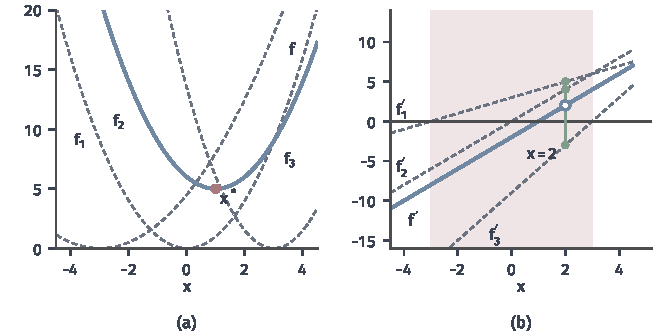
\includegraphics[width=112mm]{figures/05-optimization/05-stochastic-optimization/matplotlib/sgd-term-gradients/figure.pdf}
  \caption{三项目标~\eqref{eq:sgd-example-terms}。(a)虚线是三条单项抛物线$f_1,f_2,f_3$，实线是它们的平均$f$，红点是$f$的最小点$x^\star=1$，各项的最小点都不在这里。(b)虚线是单项导数，实线是$f'$。红底区间$[-3,3]$内三项导数不同号；区间外三项同号，都指向区间。竖线段标出$x=2$处的三个读数$5,4,-3$，空心点是它们的平均$2$。}
  \label{fig:sgd-term-gradients}
\end{BookInlineFigure}

图~\ref{fig:sgd-term-gradients}(b)给出了分歧发生的位置。三条单项导数的零点是$-3,0,3$，在这三个数之外，三项一致地指向同一边，读哪一项方向都对。进入$[-3,3]$后各项开始争执。所以离解还远时，单项读数和完整梯度方向相同；离解越近，分歧越明显。

\paragraph{归一化、正则项与读取成本}
式~\eqref{eq:sgd-finite-sum}里的$1/N$不是可有可无的约定。若目标写成不除以$N$的总和，最小点不变，但梯度和光滑常数都放大$N$倍，同一个数值的步长含义完全不同。本章一律使用平均的写法，步长$\alpha$可以脱离$N$来讨论。

许多目标还带确定的正则项$r$，例如$r(\bm{x})=\tfrac{\gamma}{2}\lVert\bm{x}\rVert_2^2$：
\begin{equation}
 f(\bm{x})=\frac{1}{N}\sum_{i=1}^{N}f_i(\bm{x})+r(\bm{x}).
 \label{eq:sgd-finite-sum-regularized}
\end{equation}
$r$不依赖数据项，它的梯度每步都能精确算出，无需抽样。读数应写成$\nabla f_i(\bm{x})+\nabla r(\bm{x})$。如果把$r$放进每一项，写成$f_i+r$，结果相同；要避免的是只在抽到某些项时才加入$r$，或把系数随$N$改变而不作说明。

计数时要分清两种成本：一次读取是对单项的梯度计算，一次更新是对$\bm{x}$的修改。完整梯度下降每次更新$N$次读取，只读一项时每次更新一次读取。比较算法时，本章以读取次数为主要的计量单位。

\subsection{期望目标}
\label{sec:sgd-expected}

很多问题中项数不是固定的$N$。观测可以源源不断地取得，或者目标本来就是在某个分布上的平均。

\paragraph{从有限平均到期望}
设$\bm{\xi}$是可以抽样的随机变量，对每个$\bm{\xi}$的取值有函数$\phi(\bm{x};\bm{\xi})$。\term{期望目标}（expected objective）是
\begin{equation}
 f(\bm{x})=\mathbb{E}_{\bm{\xi}}[\phi(\bm{x};\bm{\xi})].
 \label{eq:sgd-expected-objective}
\end{equation}
有限和是特例：取$\bm{\xi}$为均匀分布的下标$i$，$\phi(\bm{x};i)=f_i(\bm{x})$。三项目标正是这样，$f$是三点分布上的期望。

一般情况下无法把所有取值列出来，也无法求出$f$，却能抽样。这样就有两种不同的做法。

一种是\emph{直接优化期望}：每一步抽一个新样本，把它的梯度用于更新。每个样本只用一次，读取总数等于样本总数，要最小化的始终是式~\eqref{eq:sgd-expected-objective}。另一种是\emph{先固定一批样本}：一次抽定$\bm{\xi}_1,\ldots,\bm{\xi}_N$，得到
\[
 f_N(\bm{x})=\frac{1}{N}\sum_{i=1}^{N}\phi(\bm{x};\bm{\xi}_i),
\]
然后把$f_N$当作有限和目标反复读取。这时算法解的是$f_N$，它的解一般不是$f$的解。

\begin{BookInlineFigure}
  \centering
  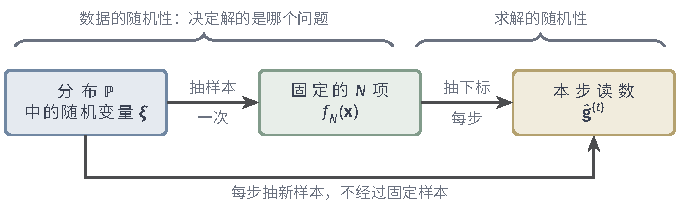
\includegraphics[width=112mm]{figures/05-optimization/05-stochastic-optimization/tikz/sgd-two-randomness/figure.pdf}
  \caption{两层随机性。上方路线先抽定$N$个样本，得到确定的有限和$f_N$，之后每步只对下标抽样。下方路线不经过固定样本，每步直接抽新样本。第一层随机性决定了算法解的是哪个问题，第二层只影响算法解这个问题的过程。}
  \label{fig:sgd-two-randomness}
\end{BookInlineFigure}

图~\ref{fig:sgd-two-randomness}区分了这两层随机性。举一个具体的例子：取$\phi(x;\xi)=\tfrac12(x-\xi)^2$，$\xi$的均值为$1$。期望目标的最小点是$1$，而$f_N$的最小点是样本均值$\bar{\xi}_N$，它随样本变化。无论优化做得多准，都只能精确得到$\bar{\xi}_N$；$\bar{\xi}_N$与$1$的差属于数据造成的统计误差。本章固定目标，只研究优化误差。统计误差的大小可参考\BookChapterRef{chap:finite-sample-error-bounds}{卷八第4章“有限样本的误差上界”}。

\paragraph{逐样本求导的条件}
随机梯度要求$\nabla\phi(\bm{x};\bm{\xi})$的期望等于$\nabla f(\bm{x})$，也就是导数和期望可以交换。有限和中这一步只是有限项相加，期望的情形需要条件。

\begin{lemma}[逐样本求导]
\label{lem:sgd-differentiate-expectation}
设$\bm{x}$有开球邻域$\bm{U}$，$\phi(\bm{x};\bm{\xi})$可积。若几乎所有$\bm{\xi}$使$\phi(\cdot;\bm{\xi})$在$\bm{U}$上可微，且存在可积函数$M(\bm{\xi})$，使
\begin{equation}
 \lVert\nabla\phi(\bm{y};\bm{\xi})\rVert_2\leq M(\bm{\xi}),\qquad \bm{y}\in\bm{U},
 \label{eq:sgd-local-domination}
\end{equation}
则$f$在$\bm{x}$处可微，并且
\begin{equation}
 \nabla f(\bm{x})=\mathbb{E}_{\bm{\xi}}[\nabla\phi(\bm{x};\bm{\xi})].
 \label{eq:sgd-gradient-expectation}
\end{equation}
\end{lemma}

\begin{proof}
记$\bm{v}(\bm{\xi})=\nabla\phi(\bm{x};\bm{\xi})$。由式~\eqref{eq:sgd-local-domination}，$\bm{v}$可积。取$\bm{h}^{(k)}\to\bm{0}$，$\bm{h}^{(k)}\neq\bm{0}$，且$\bm{x}+\bm{h}^{(k)}\in\bm{U}$，令
\[
 R_k(\bm{\xi})=\frac{\phi(\bm{x}+\bm{h}^{(k)};\bm{\xi})-\phi(\bm{x};\bm{\xi})-\langle\bm{v}(\bm{\xi}),\bm{h}^{(k)}\rangle}{\lVert\bm{h}^{(k)}\rVert_2}.
\]

对几乎所有$\bm{\xi}$，由可微性有$R_k(\bm{\xi})\to0$。沿线段使用中值定理，并由式~\eqref{eq:sgd-local-domination}，得到
\[
 \lvert R_k(\bm{\xi})\rvert\leq2M(\bm{\xi}).
\]
这说明$\phi(\bm{x}+\bm{h}^{(k)};\cdot)$也可积，$f$在这些点有定义。

控制收敛定理给出$\mathbb{E}[R_k]\to0$，定理的条件和证明见\BookChapterRef{chap:integration}{卷四第6章“积分”}。序列$\bm{h}^{(k)}$是任取的，所以这正是$f$在$\bm{x}$处以$\mathbb{E}[\bm{v}]$为梯度可微的定义。
\end{proof}

条件~\eqref{eq:sgd-local-domination}去掉后结论可以错得很彻底。取$\xi$在$(0,1)$上均匀，$\phi(x;\xi)$是示性函数：当$\xi\leq x$时取$1$，否则取$0$。对$x\in(0,1)$，期望目标是$f(x)=x$，导数处处为$1$。但对每个固定的$\xi$，除$x=\xi$这一点外函数都是常数，逐样本导数是$0$，平均之后还是$0$。跳跃点带来的贡献被逐样本求导完全漏掉了。对照引理的条件，落在$\bm{U}$内的$\xi$使$\phi(\cdot;\xi)$在$y=\xi$处不连续，“在整个邻域上可微”这一条不成立；只在$x$这一点几乎处处可微是不够的。

分布本身依赖$\bm{x}$时，式~\eqref{eq:sgd-gradient-expectation}不能直接用，因为抽样分布也在变。常用的处理是把随机性移到不依赖$\bm{x}$的变量上（重参数化），或用分布密度的对数导数作权重（得分函数估计），可参考\BookChapterRef{chap:expectation-gradient-estimation}{卷七第33章“含参期望的梯度估计”}。本章下文只讨论分布不依赖$\bm{x}$的情形。

\subsection{条件无偏与读数误差}
\label{sec:sgd-unbiased}

式~\eqref{eq:sgd-uniform-mean}是对固定的$\bm{x}$写的。迭代中$\bm{x}^{(t)}$本身由前面的抽样决定，也是随机的。需要一个能处理“当前点已经随机地到了这里”的说法。

\paragraph{历史与条件期望}
把第$t$步抽样之前已经发生的一切称为\emph{历史}，记为$\mathcal{F}^{(t)}$：初始点、前$t$次抽到的下标。给定历史，$\bm{x}^{(t)}$就是一个确定的点。条件期望$\mathbb{E}[\cdot\mid\mathcal{F}^{(t)}]$可以这样理解：把过去冻结，只对第$t$步的新抽样求平均。

本章反复使用条件期望的两条规则。历史已知的量可以提到条件期望外面：
\begin{equation}
 \mathbb{E}[\,\bm{u}^\top\bm{v}\mid\mathcal{F}^{(t)}]=\bm{u}^\top\mathbb{E}[\bm{v}\mid\mathcal{F}^{(t)}],\qquad \bm{u}\text{由}\mathcal{F}^{(t)}\text{确定}.
 \label{eq:sgd-pull-out}
\end{equation}
先对新抽样平均、再对历史平均，等于直接取总平均，即全期望公式：
\begin{equation}
 \mathbb{E}\bigl[\mathbb{E}[X\mid\mathcal{F}^{(t)}]\bigr]=\mathbb{E}[X].
 \label{eq:sgd-tower}
\end{equation}
这两条规则的一般表述和条件可参考\BookChapterRef{chap:conditional-expectation}{卷七第10章“条件期望”}。

下面把读数记作$\hat{\bm{g}}^{(t)}$，$\bm{g}^{(t)}=\nabla f(\bm{x}^{(t)})$仍表示真梯度。

\begin{definition}[条件无偏]
\label{def:sgd-unbiased}
若随机向量$\hat{\bm{g}}^{(t)}$满足
\begin{equation}
 \mathbb{E}[\hat{\bm{g}}^{(t)}\mid\mathcal{F}^{(t)}]=\nabla f(\bm{x}^{(t)}),
 \label{eq:sgd-unbiased}
\end{equation}
就称它是当前梯度的\term{条件无偏}（conditionally unbiased）估计。
\end{definition}

条件不能换成不带条件的$\mathbb{E}[\hat{\bm{g}}^{(t)}]$。在三项目标上从$x^{(0)}=2$出发，取$\alpha=0.1$。第一步的三种可能是$x^{(1)}=1.5,1.6,2.3$。若第一步抽到第三项，给定这段历史后当前点是$2.3$，第二步读数的条件均值是
\[
 \mathbb{E}[\hat{g}^{(1)}\mid\mathcal{F}^{(1)}]=f'(2.3)=2.6.
\]
不带条件地平均，则要把三种历史也平均进去，得到的是
\[
 \mathbb{E}[\hat{g}^{(1)}]=\frac{f'(1.5)+f'(1.6)+f'(2.3)}{3}=1.6.
\]
算法站在$2.3$处需要的是$2.6$这个数，$1.6$回答的是另一个问题。

\paragraph{读数的分解}
一般的读数未必无偏。把它分成三部分来记录：
\begin{equation}
 \hat{\bm{g}}^{(t)}=\nabla f(\bm{x}^{(t)})+\bm{b}^{(t)}+\bm{\zeta}^{(t)},
 \label{eq:sgd-read-decomposition}
\end{equation}
其中条件偏差和零条件均值噪声分别是
\[
 \bm{b}^{(t)}=\mathbb{E}[\hat{\bm{g}}^{(t)}\mid\mathcal{F}^{(t)}]-\nabla f(\bm{x}^{(t)}),\qquad
 \bm{\zeta}^{(t)}=\hat{\bm{g}}^{(t)}-\mathbb{E}[\hat{\bm{g}}^{(t)}\mid\mathcal{F}^{(t)}].
\]

\begin{BookInlineFigure}
  \centering
  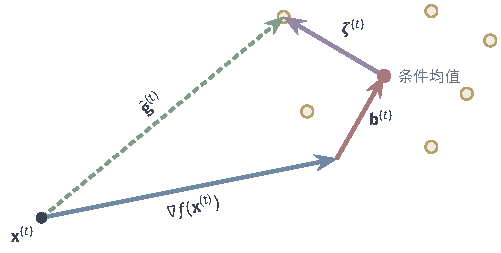
\includegraphics[width=80mm]{figures/05-optimization/05-stochastic-optimization/tikz/sgd-read-decomposition/figure.pdf}
  \caption{读数的三段分解。蓝色是真梯度，红色是条件偏差，紫色是一次读数偏离条件均值的噪声，绿色虚线是最终拿到的读数。黄色小圆是其他可能的读数，它们围绕条件均值分布。条件无偏的含义是红色线段长度为零，黄色小圆的中心落在蓝色箭头的端点上。}
  \label{fig:sgd-read-decomposition}
\end{BookInlineFigure}

图~\ref{fig:sgd-read-decomposition}说明了两部分误差的不同性质。偏差是系统性的，反复平均也去不掉；噪声的均值为零，累积时会相互抵消一部分。在二阶量上这个区别体现为交叉项消失。噪声的条件均值为零，再由规则~\eqref{eq:sgd-pull-out}，交叉项为零，于是
\begin{equation}
 \mathbb{E}[\lVert\hat{\bm{g}}^{(t)}\rVert_2^2\mid\mathcal{F}^{(t)}]
 =\lVert\nabla f(\bm{x}^{(t)})+\bm{b}^{(t)}\rVert_2^2+\mathbb{E}[\lVert\bm{\zeta}^{(t)}\rVert_2^2\mid\mathcal{F}^{(t)}].
 \label{eq:sgd-second-moment}
\end{equation}
后面的分析分别记录这两个量，噪声的条件二阶矩也称条件方差。

\paragraph{例中的偏差与方差}
三项目标上均匀抽样的读数无偏，$\bm{b}^{(t)}=0$。令$\delta=x-1$，式~\eqref{eq:sgd-example-gradients}的三个读数写成$\delta+4$，$2\delta+2$，$3\delta-6$。它们平方的平均是
\[
 \frac13\bigl[(\delta+4)^2+(2\delta+2)^2+(3\delta-6)^2\bigr]=\frac{14\delta^2-20\delta+56}{3}.
\]
减去$f'(x)^2=4\delta^2$，得到条件方差
\begin{equation}
 \sigma^2(x)=\frac{2\delta^2-20\delta+56}{3},\qquad \delta=x-1.
 \label{eq:sgd-example-variance}
\end{equation}
在$x=x^\star$处它等于$56/3\approx18.67$，这时完整梯度已经是零，噪声却最明显。在$x=2$处，$\delta=1$，方差是$38/3\approx12.67$。

式~\eqref{eq:sgd-example-variance}还说明，方差随$\lvert x\rvert\to\infty$按$\delta^2$增长。“条件方差处处不超过某个常数”这种常用假设，即使对最简单的二次目标也只在有界区域内成立。下文使用这类假设时，都理解为沿迭代点成立，它通常需要迭代点停留在有界区域内，这件事本身需要验证。

有偏的读数也容易构造。若按概率$(1/2,1/4,1/4)$抽项，又直接使用读数而不作修正，$x=2$处的条件均值是
\[
 \frac12\cdot5+\frac14\cdot4+\frac14\cdot(-3)=2.75,
\]
相对$f'(2)=2$的偏差是$0.75$。第~\ref{sec:sgd-importance}小节将说明这种偏差怎样改变实际求解的目标，以及如何用权重把它去掉。

\paragraph{无偏不保证单步下降}
条件无偏是平均意义上的性质，一次读数可能与真梯度成钝角。$x=2$处抽到第三项时，读数$-3$和真梯度$2$的乘积是$-6$，沿负读数走一步函数值上升。对比之下，条件无偏只保证
\[
 \mathbb{E}[\langle\nabla f(\bm{x}^{(t)}),\hat{\bm{g}}^{(t)}\rangle\mid\mathcal{F}^{(t)}]=\lVert\nabla f(\bm{x}^{(t)})\rVert_2^2\geq0.
\]
所以随机梯度方法不能用“每步函数值都下降”来分析，要用的是期望意义上的进展。

\subsection{循环读取与随机重排}
\label{sec:sgd-reading-orders}

上面的条件无偏依赖每步独立抽样。可在有限和目标上，常见的读取方式并不独立。

\paragraph{三种读取顺序}
有放回抽样每步独立地均匀抽一个下标，这一轮里有的项可能抽到多次，有的项可能一次也没抽到。固定循环按$1,2,\ldots,N$的顺序反复读取。\term{随机重排}（random reshuffling）每轮开始时把$N$项随机打乱一次，然后无放回地读完。把连续读取$N$项称为一\emph{轮}，后两种方式的每一轮都恰好读全部的项，图~\ref{fig:sgd-reading-orders}对比了三种方式。

\begin{BookInlineFigure}
  \centering
  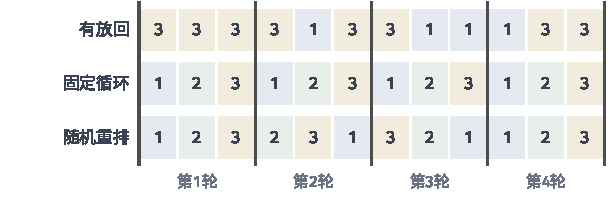
\includegraphics[width=104mm]{figures/05-optimization/05-stochastic-optimization/matplotlib/sgd-reading-orders/figure.pdf}
  \caption{三项目标在四轮内的读取顺序（种子固定）。每格的数字和底色表示读到的项，粗竖线分隔各轮。有放回抽样的一轮可能缺项、重项，固定循环每轮相同，随机重排每轮恰好各读一次，但顺序每轮不同。}
  \label{fig:sgd-reading-orders}
\end{BookInlineFigure}

\paragraph{一轮之内读数有偏}
随机重排打破了逐步条件无偏。在$x=2$处，设本轮首先读了第三项。给定这段历史，剩下两项的读数是第一项和第二项，平均后是
\[
 \frac{f_1'(2)+f_2'(2)}{2}=\frac{5+4}{2}=4.5.
\]
而完整梯度是$2$。这个偏差很好理解：读了负的一项，剩下的项一定偏正。所以式~\eqref{eq:sgd-unbiased}对随机重排的一轮内部不成立，无法直接沿用逐步的条件期望递推。

\paragraph{按整轮来分析}
偏差并不是坏事，因为一轮的总和是精确的。把一轮的$N$项读取顺序记为$\pi_0,\ldots,\pi_{N-1}$，轮内迭代点记为$\bm{x}_0,\ldots,\bm{x}_N$，步长固定为$\alpha$。把每一步的读数在轮初的点$\bm{x}_0$处展开，
\[
 \bm{x}_N=\bm{x}_0-\alpha\sum_{k=0}^{N-1}\nabla f_{\pi_k}(\bm{x}_k).
\]
一轮恰好读全部的项，所以各项读数在同一点$\bm{x}_0$处的和就是$N$倍的完整梯度。在每一项里加减$\nabla f_{\pi_k}(\bm{x}_0)$，得到
\begin{equation}
 \bm{x}_N=\bm{x}_0-\alpha N\nabla f(\bm{x}_0)-\alpha\sum_{k=0}^{N-1}\bigl[\nabla f_{\pi_k}(\bm{x}_k)-\nabla f_{\pi_k}(\bm{x}_0)\bigr].
 \label{eq:sgd-epoch-expansion}
\end{equation}
第一部分恰是步长$\alpha N$的一次完整梯度下降，与顺序无关。若各项梯度$L_i$-Lipschitz，第二部分的每一项不超过$L_i\lVert\bm{x}_k-\bm{x}_0\rVert_2$，而$\lVert\bm{x}_k-\bm{x}_0\rVert_2$本身是$\alpha$的量级，所以这部分是$\alpha^2$的量级。

一轮之内读到的梯度并不消失，它们的噪声在一轮结束时几乎抵消。有放回抽样没有这个结构，每步噪声$\alpha\bm{\zeta}^{(t)}$是$\alpha$的量级，一轮的总噪声还是$\alpha$的量级。

三项目标可以直接核对。从$x_0=2$开始，步长$\alpha=0.1$，顺序为$3,1,2$，轮内的点依次是$2.3,\ 1.77,\ 1.416$。式~\eqref{eq:sgd-epoch-expansion}的第一部分给出
\[
 2-0.1\cdot3\cdot2=1.4.
\]
第二部分的三项里，第三项在$x_0$处读取，差为零；第一项在$2.3$处读取，差是$1\cdot0.3$；第二项在$1.77$处读取，差是$2\cdot(-0.23)$。所以第二部分是
\[
 -0.1\cdot(0+0.3-0.46)=0.016,
\]
两部分合计$1.416$，与逐步计算一致。

\begin{BookInlineFigure}
  \centering
  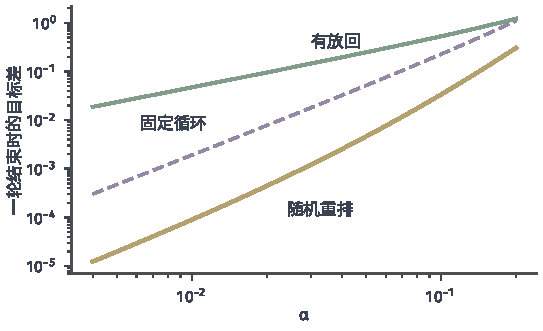
\includegraphics[width=92mm]{figures/05-optimization/05-stochastic-optimization/matplotlib/sgd-epoch-floor/figure.pdf}
  \caption{三项目标上固定步长运行至稳定后，一轮结束时的期望目标差与步长的关系，两轴都取对数。数值由精确递推算出，并非抽样估计。绿线是有放回抽样，紫色虚线是固定顺序$1,2,3$，黄线是随机重排。}
  \label{fig:sgd-epoch-floor}
\end{BookInlineFigure}

图~\ref{fig:sgd-epoch-floor}比较了固定步长长期运行后的误差。图中的三条直线斜率不同：步长缩小十倍时，有放回抽样的目标差约缩小十倍；固定循环约缩小一百倍；随机重排缩小的倍数更大，在$\alpha=0.1$和$0.01$之间约为三百七十倍，曲线向千倍的斜率靠近。在$\alpha=0.01$时，三者的目标差依次约为$4.7\times10^{-2}$，$1.9\times10^{-3}$，$9.0\times10^{-5}$。

固定循环的误差是一个确定的偏移，步长固定后迭代点按周期收敛到一条轨道，其离$x^\star$的距离是$\alpha$的量级，目标差是$\alpha^2$的量级，而且偏移大小与读取顺序有关。随机重排把各种顺序平均，轮末偏移的主要部分相互抵消。

这张图只来自一个二次例子，斜率不能直接当作一般定理。一般目标上，随机重排的结论需要对一轮的累积偏差单独分析，证明较长，读者可查阅相关文献。本章后面的逐步分析都针对有放回抽样或新样本的情形，把它们用于随机重排时要注意上面的差别。

\section{随机梯度方法}
\label{sec:sgd-method}

上一节说清了读数和真梯度的关系。这就需要回答：把读数直接放进梯度更新后，有限步之内能保证什么？答案由三件事决定：抽样和步长的先后，步长的大小随时间怎样变化，以及最后返回哪个点。

\subsection{随机梯度下降}
\label{sec:sgd-basic}

\paragraph{主要思想}
把梯度下降式中的$\nabla f(\bm{x}^{(t)})$换成读数，就得到\term{随机梯度下降}（stochastic gradient descent）：
\begin{equation}
 \begin{gathered}
 \bm{x}^{(t+1)}=\bm{x}^{(t)}-\alpha^{(t)}\hat{\bm{g}}^{(t)},\\
 \hat{\bm{g}}^{(t)}=\nabla f_{i^{(t)}}(\bm{x}^{(t)}).
 \end{gathered}
 \label{eq:sgd-update}
\end{equation}
$i^{(t)}$是第$t$步抽到的下标，对期望目标则换成新样本$\bm{\xi}^{(t)}$。

可以把它想成下山时每一步只问一位向导。每位向导都有自己的偏好，单独听一位可能走错，但向导们的平均意见是对的。步子小时，连走许多步的总位移接近多位意见的累积，错误相互抵消，走的是平均路线。这个类比说明步长必须小：步子大时一次错误就走出很远，后面来不及纠正。

式~\eqref{eq:sgd-update}的执行顺序有讲究。基本分析要求$\alpha^{(t)}$在抽取$i^{(t)}$之前已经确定，也就是$\alpha^{(t)}$由历史$\mathcal{F}^{(t)}$决定。这样在条件期望中它可以提到外面，式~\eqref{eq:sgd-pull-out}才能用。

\needspace{6\baselineskip}
\paragraph{变量}
\begin{itemize}
 \item $\bm{x}^{(t)}\in\mathbb{R}^n$：当前点，在原处更新。
 \item $i^{(t)}$：本步抽到的下标，用完即弃。
 \item $\hat{\bm{g}}^{(t)}\in\mathbb{R}^n$：本步读数。
 \item $\alpha^{(t)}>0$：本步步长，抽样前确定。
 \item $\hat{\bm{x}}$：最后返回的点，是最后一个迭代点还是某种平均，后面讨论。
\end{itemize}

\paragraph{初始化}
选定初始点、步长规则和总步数$T$。例中取
\[
 x^{(0)}=2,\qquad \alpha=0.1,
\]
并设前三步抽到的下标依次是$3,1,2$。

\paragraph{每轮更新}
对$t=0,1,\ldots,T-1$依次执行以下步骤。

\begin{enumerate}
 \item 抽样：独立地均匀抽取下标$i^{(t)}$。例中第一轮$i^{(0)}=3$。
 \item 读取：计算本项在当前点的梯度，作为读数$\hat{\bm{g}}^{(t)}$。例中第一轮由式~\eqref{eq:sgd-example-gradients}，
 \[
  \hat{g}^{(0)}=3\cdot2-9=-3.
 \]
 \item 更新：由式~\eqref{eq:sgd-update}计算新点。例中第一轮
 \[
  x^{(1)}=2-0.1\cdot(-3)=2.3.
 \]
 目标差从$1$变成$1.69$，这一步走了上坡。
 \item 记录：保存计算输出所需的量。若返回平均点，这里累加$\alpha^{(t)}\bm{x}^{(t)}$和$\alpha^{(t)}$；例中只保留当前点。
\end{enumerate}

例中第二轮$i^{(1)}=1$，读数和新点是
\[
 \hat{g}^{(1)}=2.3+3=5.3,\qquad x^{(2)}=2.3-0.53=1.77.
\]

例中第三轮$i^{(2)}=2$，读数和新点是
\[
 \hat{g}^{(2)}=2\cdot1.77=3.54,\qquad x^{(3)}=1.77-0.354=1.416.
\]

迭代在预定的$T$步后结束。随机梯度不能用$\lVert\hat{\bm{g}}^{(t)}\rVert_2$作停止判据，因为它在最优点也不趋于零。最终得到$\hat{\bm{x}}$，例中经过三次读取得到$x^{(3)}=1.416$，目标差降到$0.173$。这三次读取的总量等于一次完整梯度的成本。

\paragraph{单步分析：下降量和噪声项}
一次更新的后果可以分成两部分：沿真梯度走带来的下降，和读数抖动带来的损失。把更新代入第~\ref{chap:smooth-foundations}章的下降引理就能把它们分开。

\begin{theorem}[单步期望进展]
\label{thm:sgd-one-step}
设$f$的梯度$L$-Lipschitz，读数满足条件无偏~\eqref{eq:sgd-unbiased}，$\sigma_t^2$是噪声$\bm{\zeta}^{(t)}$的条件方差，$\alpha^{(t)}$由$\mathcal{F}^{(t)}$确定。则
\begin{equation}
 \begin{aligned}
 \mathbb{E}[f(\bm{x}^{(t+1)})\mid\mathcal{F}^{(t)}]
 \leq{}&f(\bm{x}^{(t)})-\alpha^{(t)}\Bigl(1-\frac{L\alpha^{(t)}}{2}\Bigr)\lVert\nabla f(\bm{x}^{(t)})\rVert_2^2\\
 &+\frac{L(\alpha^{(t)})^2}{2}\sigma_t^2.
 \end{aligned}
 \label{eq:sgd-one-step}
\end{equation}
\end{theorem}

\begin{proof}
证明中省略迭代编号，把当前点、步长和读数简记为$\bm{x},\alpha,\hat{\bm{g}}$。在下降引理中取$\bm{y}=\bm{x}-\alpha\hat{\bm{g}}$，得到
\[
 f(\bm{x}-\alpha\hat{\bm{g}})\leq f(\bm{x})-\alpha\langle\nabla f(\bm{x}),\hat{\bm{g}}\rangle+\frac{L\alpha^2}{2}\lVert\hat{\bm{g}}\rVert_2^2.
\]

对两边取$\mathbb{E}[\cdot\mid\mathcal{F}^{(t)}]$。$\bm{x}$和$\alpha$由历史确定，提到外面。由条件无偏，内积项的条件期望是
\[
 \mathbb{E}[\langle\nabla f(\bm{x}),\hat{\bm{g}}\rangle\mid\mathcal{F}^{(t)}]=\lVert\nabla f(\bm{x})\rVert_2^2.
\]

由式~\eqref{eq:sgd-second-moment}，取$\bm{b}^{(t)}=\bm{0}$，二次项的条件期望是
\[
 \mathbb{E}[\lVert\hat{\bm{g}}\rVert_2^2\mid\mathcal{F}^{(t)}]=\lVert\nabla f(\bm{x})\rVert_2^2+\sigma_t^2.
\]
两式代入后合并$\lVert\nabla f(\bm{x})\rVert_2^2$的系数，即得式~\eqref{eq:sgd-one-step}。
\end{proof}

和完整梯度的下降估计相比，式~\eqref{eq:sgd-one-step}只多了右端最后一项。它与$\alpha^2$成正比，而下降量大体与$\alpha$成正比，所以步长足够小时下降占优。接近解时$\lVert\nabla f\rVert_2$变小，下降量随之变小，噪声项却不减。两者相等的位置，就是算法再也走不动的地方。

用三项目标从$x^{(0)}=2$走一步，看这个不等式的两部分。图~\ref{fig:sgd-single-step}画出了三种可能的结果。三个读数给出的新点和目标差分别是
\[
 x^{(1)}=1.5,\ 1.6,\ 2.3,\qquad (x^{(1)}-1)^2=0.25,\ 0.36,\ 1.69.
\]
抽到第三项时目标差从$1$上升到$1.69$，三种结果的平均却下降了：
\[
 \frac{0.25+0.36+1.69}{3}\approx0.767.
\]

\begin{BookInlineFigure}
  \centering
  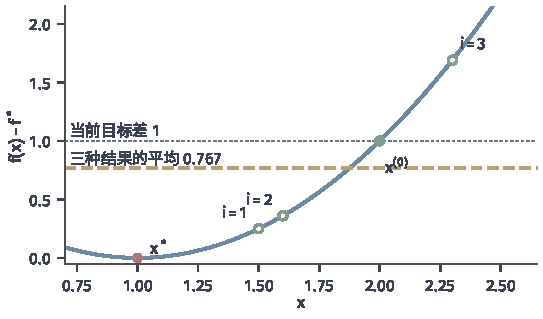
\includegraphics[width=92mm]{figures/05-optimization/05-stochastic-optimization/matplotlib/sgd-single-step/figure.pdf}
  \caption{单步的三种结果。蓝线是目标差$(x-1)^2$，实心绿点是当前点$x^{(0)}=2$，空心绿点是抽到第$i$项后的新点，步长$\alpha=0.1$。第三项使目标差上升到$1.69$，其余两项使它下降。虚线是三种结果的平均$0.767$，低于当前目标差$1$。}
  \label{fig:sgd-single-step}
\end{BookInlineFigure}

式~\eqref{eq:sgd-one-step}给出的数值是相同的。这里$L=2$，$\lvert f'(2)\rvert=2$，条件方差由式~\eqref{eq:sgd-example-variance}是$38/3$，所以下降量和噪声项分别是
\[
 0.1\cdot(1-0.1)\cdot4=0.36,\qquad 0.01\cdot\frac{38}{3}\approx0.127.
\]
于是
\[
 1-0.36+0.127=0.767.
\]
目标是二次函数，下降引理取等号，理论值与实际值完全相同。

\subsection{步长调度}
\label{sec:sgd-step-schedule}

单步分析留下一个问题：步长选大了噪声项大，选小了下降量小，$\alpha^{(t)}$该如何随$t$变化？

\paragraph{固定步长：收敛到一个邻域}
先看步长不变时发生什么。在强凸目标上，初始误差按几何速度消退，噪声则把误差托在一个不为零的水平。

\begin{theorem}[固定步长的误差邻域]
\label{thm:sgd-constant-step}
设$f$的梯度$L$-Lipschitz且$f$是$\mu$强凸的，读数条件无偏，且沿迭代点$\sigma_t^2\leq\sigma^2$。若固定步长$0<\alpha\leq1/L$，则对所有$T\geq0$，
\begin{equation}
 \mathbb{E}[f(\bm{x}^{(T)})]-f^\star\leq(1-\alpha\mu)^T\bigl(f(\bm{x}^{(0)})-f^\star\bigr)+\frac{\alpha L\sigma^2}{2\mu}.
 \label{eq:sgd-constant-step}
\end{equation}
\end{theorem}

\begin{proof}
记$e_t=\mathbb{E}[f(\bm{x}^{(t)})]-f^\star$。因为$\alpha L\leq1$，所以$1-L\alpha/2\geq1/2$，式~\eqref{eq:sgd-one-step}给出
\[
 \mathbb{E}[f(\bm{x}^{(t+1)})\mid\mathcal{F}^{(t)}]\leq f(\bm{x}^{(t)})-\frac{\alpha}{2}\lVert\nabla f(\bm{x}^{(t)})\rVert_2^2+\frac{L\alpha^2}{2}\sigma^2.
\]

强凸性给出对任意$\bm{x},\bm{y}$成立的下界
\[
 f(\bm{y})\geq f(\bm{x})+\langle\nabla f(\bm{x}),\bm{y}-\bm{x}\rangle+\frac{\mu}{2}\lVert\bm{y}-\bm{x}\rVert_2^2.
\]
右端对$\bm{y}$最小化，最小值在$\bm{y}=\bm{x}-\nabla f(\bm{x})/\mu$处取得，所以
\[
 f^\star\geq f(\bm{x})-\frac{1}{2\mu}\lVert\nabla f(\bm{x})\rVert_2^2.
\]
这就是
\[
 \lVert\nabla f(\bm{x})\rVert_2^2\geq2\mu\bigl(f(\bm{x})-f^\star\bigr).
\]

把这个下界代入第一个不等式，两边减去$f^\star$，再取全期望~\eqref{eq:sgd-tower}，得到递推
\[
 e_{t+1}\leq(1-\alpha\mu)e_t+\frac{L\alpha^2\sigma^2}{2}.
\]

由$\alpha\mu\leq\mu/L\leq1$，系数$1-\alpha\mu$非负，递推可以展开$T$次，得到
\[
 e_T\leq(1-\alpha\mu)^Te_0+\frac{L\alpha^2\sigma^2}{2}\sum_{k=0}^{T-1}(1-\alpha\mu)^k.
\]
几何级数不超过$1/(\alpha\mu)$，代入即得式~\eqref{eq:sgd-constant-step}。
\end{proof}

式~\eqref{eq:sgd-constant-step}的第一项随$T$消退，第二项不消退，称为\term{噪声底}（noise floor）。三个条件各有作用：光滑性使下降引理可用，强凸性把梯度大小换算成目标差，方差上界控制每步的损失。去掉强凸性，这个几何递推就不成立；去掉方差上界，噪声项无法用常数控制。

\paragraph{例中的精确递推}
三项目标可以把期望完全算出来。令$\delta_t=x^{(t)}-1$，由$x^{(t+1)}-1=\delta_t-\alpha\hat{g}^{(t)}$和式~\eqref{eq:sgd-example-variance}，条件期望分别是
\[
 \mathbb{E}[\delta_{t+1}\mid\mathcal{F}^{(t)}]=(1-2\alpha)\delta_t,
\]
\[
 \mathbb{E}[\delta_{t+1}^2\mid\mathcal{F}^{(t)}]=\Bigl(1-4\alpha+\frac{14}{3}\alpha^2\Bigr)\delta_t^2-\frac{20}{3}\alpha^2\delta_t+\frac{56}{3}\alpha^2.
\]

当$\alpha<6/7$时，$\delta_t^2$的系数小于$1$，且$\mathbb{E}[\delta_t]\to0$。令$\mathbb{E}[\delta_t^2]$的稳态值为$s$，在第二式中取全期望并令$\mathbb{E}[\delta_t]=0$，它满足
\[
 \Bigl(4\alpha-\frac{14}{3}\alpha^2\Bigr)s=\frac{56}{3}\alpha^2.
\]
解得
\begin{equation}
 \lim_{t\to\infty}\mathbb{E}[f(x^{(t)})-f^\star]=\frac{28\alpha}{6-7\alpha}.
 \label{eq:sgd-example-floor}
\end{equation}
$\alpha=0.1$时噪声底约为$0.528$，$\alpha=0.02$时约为$0.096$。

\begin{BookInlineFigure}
  \centering
  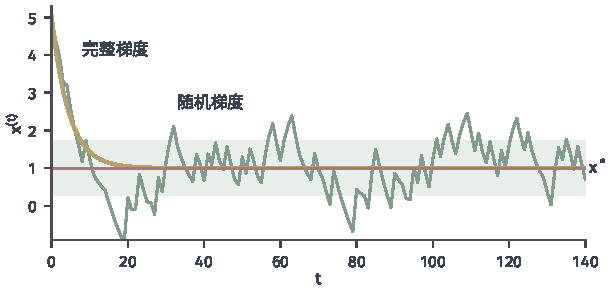
\includegraphics[width=104mm]{figures/05-optimization/05-stochastic-optimization/matplotlib/sgd-sample-path/figure.pdf}
  \caption{三项目标上从$x^{(0)}=5$出发，步长$\alpha=0.1$（种子固定）的一条路径。绿线是随机梯度，黄线是完整梯度，红线是$x^\star=1$。绿底带的半宽是式~\eqref{eq:sgd-example-floor}的平方根$0.727$，即稳态下均方根偏差。}
  \label{fig:sgd-sample-path}
\end{BookInlineFigure}

图~\ref{fig:sgd-sample-path}是一条实际路径。开始的十几步里绿线和黄线几乎重合：离解很远时信号强于噪声，抽到哪一项都往下走。之后黄线停在解上，绿线在一条带内不停抖动，这条带就是噪声底的样子。

\paragraph{固定、递减与分段}
固定步长的两部分误差互相拉扯：大的$\alpha$使初始误差消得快，噪声底却高；小的$\alpha$相反。要想噪声底趋于零，步长就得逐渐减小。

经典的递减条件是
\begin{equation}
 \sum_{t=0}^{\infty}\alpha^{(t)}=\infty,\qquad\sum_{t=0}^{\infty}(\alpha^{(t)})^2<\infty.
 \label{eq:sgd-robbins-monro}
\end{equation}
第一个要求表示累计可走的距离没有上限，初始点再远也到得了；第二个要求表示噪声积累的总量有限\scite{math-robbins1951stochastic}。例如$\alpha^{(t)}=c/(t+t_0)$同时满足两者。

分段调整介于两者之间：先用较大的步长，到达噪声底后减半，再走一段。每段把噪声底压低一半，代价是每段需要的步数翻倍。图~\ref{fig:sgd-step-schedules}(a)比较了几种调度，图中的曲线由递推精确算出。

\begin{BookInlineFigure}
  \centering
  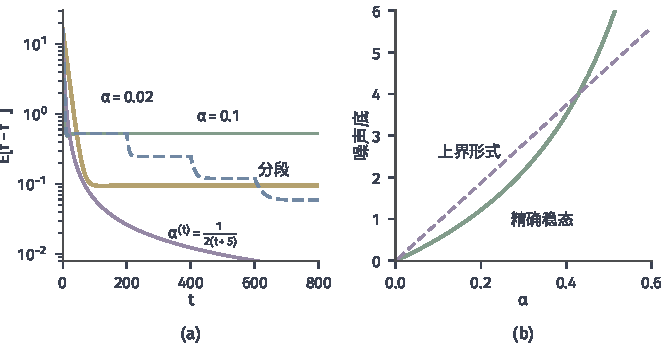
\includegraphics[width=112mm]{figures/05-optimization/05-stochastic-optimization/matplotlib/sgd-step-schedules/figure.pdf}
  \caption{三项目标的步长调度，由精确递推算出，$x^{(0)}=5$。(a)绿线和黄线是固定步长$0.1$和$0.02$，紫线是$\alpha^{(t)}=1/(2(t+5))$，蓝色虚线是从$0.1$起每$200$步减半。固定步长最后变平，大步长到得早而停得高；递减步长持续下降。(b)绿线是噪声底的精确值~\eqref{eq:sgd-example-floor}，紫色虚线是式~\eqref{eq:sgd-constant-step}第二项取$\sigma^2=56/3$的形式；后者只代入最优点处的方差，并非严格上界。步长较大时迭代离解较远，实际方差更大，绿线超过虚线。}
  \label{fig:sgd-step-schedules}
\end{BookInlineFigure}

\paragraph{时间单位}
调度写成$t$的函数时，要说明$t$计的是什么。常见的单位有三种：更新次数、读取的样本量、完整遍历的轮数。批量为$B$、项数为$N$时，一轮是$N/B$次更新，读取$N$个样本。

同一句“每200步减半”，用更新次数计时，批量改变后读取量不同；用样本量计时，批量改变后更新次数不同。批量、并行度或数据量一变，换算不当的调度含义就变了。式~\eqref{eq:sgd-constant-step}和式~\eqref{eq:sgd-robbins-monro}中的$t$都是更新次数。

\paragraph{步长依赖本轮读数时}
前面一直要求$\alpha^{(t)}$在抽样之前确定。步长若依赖本轮读数，$\mathbb{E}[\alpha^{(t)}\hat{\bm{g}}^{(t)}\mid\mathcal{F}^{(t)}]$不再等于$\alpha^{(t)}\nabla f(\bm{x}^{(t)})$，因为步长和方向相关。

在三项目标上看一个具体的后果。取只保留读数符号的规则，步长$\alpha/\lvert\hat{g}\rvert$，每步走固定距离。在$x=0.5$处，三个读数是$3.5,1,-7.5$，真梯度是$-1$，应该向右走。这三个读数的符号是两正一负，平均更新是
\[
 -\alpha\cdot\frac{1+1-1}{3}=-\frac{\alpha}{3},
\]
平均向左走，方向错了。

\begin{BookInlineFigure}
  \centering
  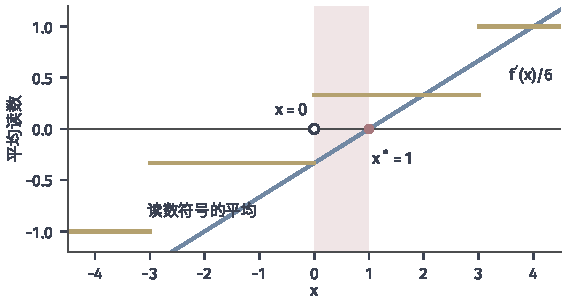
\includegraphics[width=96mm]{figures/05-optimization/05-stochastic-optimization/matplotlib/sgd-normalized-bias/figure.pdf}
  \caption{步长与读数相关时平均方向可能错误。蓝线是真梯度$f'(x)$按比例缩小$6$倍，零点是$x^\star=1$；黄色阶梯是三个读数符号的平均，零点是$x=0$。红底区间$(0,1)$内两者异号，按读数符号走的平均方向与真梯度相反。}
  \label{fig:sgd-normalized-bias}
\end{BookInlineFigure}

图~\ref{fig:sgd-normalized-bias}说明了问题的严重性：这条规则的平均动力学的零点是$x=0$，即各项最小点$-3,0,3$的中位数，而不是$x^\star=1$。缩小$\alpha$也改变不了这一点，因为偏差存在于平均方向之中。依赖读数的步长并非都不能用，后文讨论的方法多属于这一类，但必须分别分析步长与方向的相关性。

\subsection{凸目标的误差与输出}
\label{sec:sgd-convex}

前面的噪声底结论依赖强凸性。对一般的凸目标，$f-f^\star$与梯度大小没有固定的换算关系，下降引理的路线走不通。这一小节换一个量来追踪：到最优解的距离。

\paragraph{距离递推与平均点}
距离的好处是展开之后能用凸性。把更新代入$\lVert\bm{x}^{(t+1)}-\bm{x}^\star\rVert_2^2$，内积项由凸性转成目标差，所得到的结论是对迭代点的加权和成立的。

为了从加权和回到一个点，需要Jensen不等式：若$f$凸，$\lambda_t\geq0$，$\sum_t\lambda_t=1$，则
\[
 f\Bigl(\sum_t\lambda_t\bm{x}^{(t)}\Bigr)\leq\sum_t\lambda_tf(\bm{x}^{(t)}).
\]
两个点的情形就是凸函数的定义，多个点时对点数作归纳即得。

\begin{theorem}[凸目标的加权平均点]
\label{thm:sgd-convex}
设$f$凸且可微，存在最小点$\bm{x}^\star$，读数条件无偏，且沿迭代点读数的条件二阶矩不超过$G^2$，步长$\alpha^{(t)}>0$事先确定。记$R=\lVert\bm{x}^{(0)}-\bm{x}^\star\rVert_2$，$A_T=\sum_{t=0}^{T-1}\alpha^{(t)}$，加权平均点
\begin{equation}
 \bar{\bm{x}}^{(T)}=\frac{1}{A_T}\sum_{t=0}^{T-1}\alpha^{(t)}\bm{x}^{(t)}.
 \label{eq:sgd-weighted-average}
\end{equation}
则
\begin{equation}
 \mathbb{E}[f(\bar{\bm{x}}^{(T)})]-f^\star\leq\frac{R^2+G^2\sum_{t=0}^{T-1}(\alpha^{(t)})^2}{2A_T}.
 \label{eq:sgd-convex-bound}
\end{equation}
\end{theorem}

\begin{proof}
记$d_t$为$\lVert\bm{x}^{(t)}-\bm{x}^\star\rVert_2^2$的期望。展开平方，得到
\[
 \lVert\bm{x}^{(t+1)}-\bm{x}^\star\rVert_2^2=\lVert\bm{x}^{(t)}-\bm{x}^\star\rVert_2^2-2\alpha^{(t)}\langle\hat{\bm{g}}^{(t)},\bm{x}^{(t)}-\bm{x}^\star\rangle+(\alpha^{(t)})^2\lVert\hat{\bm{g}}^{(t)}\rVert_2^2.
\]

取$\mathbb{E}[\cdot\mid\mathcal{F}^{(t)}]$。$\bm{x}^{(t)}-\bm{x}^\star$由历史确定，内积项由条件无偏变成$\langle\nabla f(\bm{x}^{(t)}),\bm{x}^{(t)}-\bm{x}^\star\rangle$。凸性给出
\[
 \langle\nabla f(\bm{x}^{(t)}),\bm{x}^{(t)}-\bm{x}^\star\rangle\geq f(\bm{x}^{(t)})-f^\star.
\]

再用二阶矩的上界并取全期望，得到递推
\[
 d_{t+1}\leq d_t-2\alpha^{(t)}\bigl(\mathbb{E}[f(\bm{x}^{(t)})]-f^\star\bigr)+(\alpha^{(t)})^2G^2.
\]

对$t=0,\ldots,T-1$求和，左右的$d_t$逐项相消，再丢掉非负的$d_T$，得到
\[
 2\sum_{t=0}^{T-1}\alpha^{(t)}\bigl(\mathbb{E}[f(\bm{x}^{(t)})]-f^\star\bigr)\leq R^2+G^2\sum_{t=0}^{T-1}(\alpha^{(t)})^2.
\]

两边除以$2A_T$，并对$\lambda_t=\alpha^{(t)}/A_T$使用Jensen不等式，即得式~\eqref{eq:sgd-convex-bound}。
\end{proof}

固定步长$\alpha$时，式~\eqref{eq:sgd-convex-bound}的右端是$R^2/(2\alpha T)+\alpha G^2/2$。对$\alpha$求最小，取$\alpha=R/(G\sqrt{T})$，得到
\begin{equation}
 \mathbb{E}[f(\bar{\bm{x}}^{(T)})]-f^\star\leq\frac{RG}{\sqrt{T}}.
 \label{eq:sgd-convex-rate}
\end{equation}
要把目标差减小十倍，步数要增加一百倍。

二阶矩的上界$G^2$包含了梯度本身，在全空间常常不成立。若$f$还有$L$-Lipschitz梯度，条件可以放宽为条件方差不超过$\sigma^2$。在凸的$L$-光滑函数上，从$\bm{x}$走一步$\bm{x}-\nabla f(\bm{x})/L$，由下降引理，
\[
 f^\star\leq f(\bm{x})-\frac{1}{2L}\lVert\nabla f(\bm{x})\rVert_2^2.
\]
于是梯度大小被目标差控制，读数的二阶矩满足
\[
 \mathbb{E}[\lVert\hat{\bm{g}}^{(t)}\rVert_2^2\mid\mathcal{F}^{(t)}]\leq2L\bigl(f(\bm{x}^{(t)})-f^\star\bigr)+\sigma^2.
\]

把它代入上面的递推，当$\alpha\leq1/(2L)$时，由$1-\alpha L\geq1/2$，同样的求和给出
\begin{equation}
 \mathbb{E}[f(\bar{\bm{x}}^{(T)})]-f^\star\leq\frac{R^2}{\alpha T}+\alpha\sigma^2.
 \label{eq:sgd-convex-smooth}
\end{equation}
取$\alpha=\min\{1/(2L),R/(\sigma\sqrt{T})\}$，右端不超过$2LR^2/T+2R\sigma/\sqrt{T}$。第一项是完整梯度下降的速率，第二项是噪声带来的代价；$\sigma=0$时退回确定情形。

\paragraph{强凸性的改善}
强凸性使距离递推有了收缩，步长可以取到$1/t$的量级。

\begin{theorem}[强凸目标的递减步长]
\label{thm:sgd-strong-decay}
设$f$可微且$\mu$强凸，读数条件无偏，沿迭代点读数的条件二阶矩不超过$G^2$，$\alpha^{(t)}=1/(\mu(t+1))$。则对所有$T\geq1$，
\begin{equation}
 \mathbb{E}[\lVert\bm{x}^{(T)}-\bm{x}^\star\rVert_2^2]\leq\frac{G^2}{\mu^2T}.
 \label{eq:sgd-strong-rate}
\end{equation}
\end{theorem}

\begin{proof}
强凸下界中分别取$(\bm{x},\bm{x}^\star)$和$(\bm{x}^\star,\bm{x})$，相加并用$\nabla f(\bm{x}^\star)=\bm{0}$，得到
\[
 \langle\nabla f(\bm{x}),\bm{x}-\bm{x}^\star\rangle\geq\mu\lVert\bm{x}-\bm{x}^\star\rVert_2^2.
\]
沿用定理~\ref{thm:sgd-convex}证明中的展开，得到
\[
 d_{t+1}\leq(1-2\alpha^{(t)}\mu)d_t+(\alpha^{(t)})^2G^2=\Bigl(1-\frac{2}{t+1}\Bigr)d_t+\frac{G^2}{\mu^2(t+1)^2}.
\]

对$T$作归纳。$T=1$时，取$t=0$，系数是$-1$，由$d_0\geq0$有$d_1\leq G^2/\mu^2$，结论成立。

设$d_t\leq G^2/(\mu^2t)$，其中$t\geq1$，此时系数$1-2/(t+1)$非负。代入递推，得到
\[
 d_{t+1}\leq\frac{G^2}{\mu^2}\Bigl[\frac{t-1}{t(t+1)}+\frac{1}{(t+1)^2}\Bigr].
\]

只需证明方括号不超过$1/(t+1)$，即$\tfrac{t-1}{t}+\tfrac{1}{t+1}\leq1$。这等价于$\tfrac{1}{t+1}\leq\tfrac{1}{t}$，成立。
\end{proof}

强凸假设和全空间的$G^2$是矛盾的，因为强凸函数的梯度无界。定理中的条件要理解为迭代点在有界集内，通常由投影到有界闭凸集来保证，投影不增大到$\bm{x}^\star$的距离，上面的递推继续成立。

把结论总结成对比：

\begin{BookInlineTable}
  \centering
  \begin{tabular}{lll}
    \toprule
    条件 & 步长 & 期望误差\\
    \midrule
    凸，二阶矩有界 & $\dfrac{R}{G\sqrt{T}}$ & 平均点目标差$\dfrac{RG}{\sqrt{T}}$\\\addlinespace[2.5mm]
    凸，光滑，方差有界 & $\min\Bigl\{\dfrac{1}{2L},\dfrac{R}{\sigma\sqrt{T}}\Bigr\}$ & 平均点目标差$\dfrac{2LR^2}{T}+\dfrac{2R\sigma}{\sqrt{T}}$\\\addlinespace[2.5mm]
    强凸，二阶矩有界 & $\dfrac{1}{\mu(t+1)}$ & 末点距离平方$\dfrac{G^2}{\mu^2T}$\\\addlinespace[2.5mm]
    强凸，光滑，方差有界 & 固定，$\alpha\leq\dfrac1L$ & 末点目标差，含噪声底\\
    \bottomrule
  \end{tabular}
  \caption{本小节及上一小节的保证。表中“末点”指最后一个迭代点，“光滑”指梯度$L$-Lipschitz。前两行的结论针对平均点，后两行针对末点。}
  \label{tab:sgd-rates}
\end{BookInlineTable}

\paragraph{最后一点与平均点}
定理~\ref{thm:sgd-convex}的保证属于平均点，不能搬到任意一个迭代点上。平均值小只说明大多数项小：序列$0,0,\ldots,0,3$的平均可以任意小，而最后一项是$3$。一般凸目标上最后一点的保证需要单独证明，所得的速率通常比平均点差，具体分析较长，读者可查阅专门的文献。

\begin{BookInlineFigure}
  \centering
  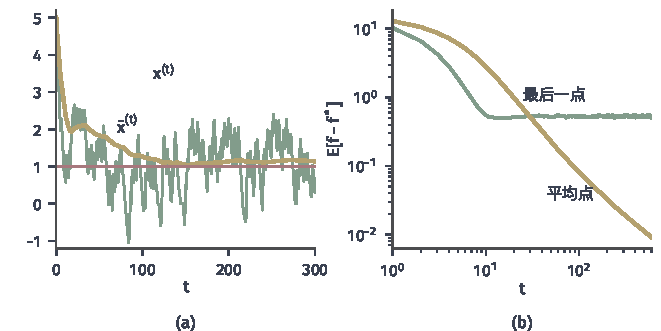
\includegraphics[width=112mm]{figures/05-optimization/05-stochastic-optimization/matplotlib/sgd-average-vs-last/figure.pdf}
  \caption{三项目标上固定步长$\alpha=0.1$，从$x^{(0)}=5$出发。(a)同一条路径上最后一点$x^{(t)}$（绿）和从头算起的平均点$\bar{x}^{(t)}$（黄），红线是$x^\star$。(b)$4000$次独立运行的平均目标差（种子固定），两轴取对数。$t=600$时最后一点的目标差约为$0.53$，平均点约为$0.009$。}
  \label{fig:sgd-average-vs-last}
\end{BookInlineFigure}

在三项目标上平均的作用很明显。图~\ref{fig:sgd-average-vs-last}(a)的绿线一直在抖，黄线很快贴近解。(b)说明最后一点停在噪声底$0.53$，平均点的目标差继续下降。原因是抖动在解的两侧来回，平均时相互抵消，而初始段的影响被越来越多的项稀释。平均点要付出的代价是多存一个向量，并且受早期迭代点的拖累，因此实践中也常只平均后面一段。

\subsection{非凸目标的误差与输出}
\label{sec:sgd-nonconvex}

目标非凸时，到最小点的距离既不能保证下降，也可能不止一个最小点。只能回到单步下降，评价的量也要换成梯度大小。

\paragraph{累加下降量}
式~\eqref{eq:sgd-one-step}不需要凸性，把它沿$t$累加，左边望远镜相消，剩下函数值的总下降量，它受目标下界限制。

\begin{theorem}[非凸目标的平均平方梯度]
\label{thm:sgd-nonconvex}
设$f$有下界$f_{\inf}$，梯度$L$-Lipschitz，读数条件无偏且沿迭代点$\sigma_t^2\leq\sigma^2$，步长事先确定且$0<\alpha^{(t)}\leq1/L$。记$\Delta=f(\bm{x}^{(0)})-f_{\inf}$，$A_T=\sum_{t=0}^{T-1}\alpha^{(t)}$。则
\begin{equation}
 \frac{1}{A_T}\sum_{t=0}^{T-1}\alpha^{(t)}\mathbb{E}[\lVert\nabla f(\bm{x}^{(t)})\rVert_2^2]\leq\frac{2\Delta+L\sigma^2\sum_{t=0}^{T-1}(\alpha^{(t)})^2}{A_T}.
 \label{eq:sgd-nonconvex-bound}
\end{equation}
\end{theorem}

\begin{proof}
由$\alpha^{(t)}L\leq1$，式~\eqref{eq:sgd-one-step}的系数$1-L\alpha^{(t)}/2\geq1/2$。取全期望，得到
\[
 \frac{\alpha^{(t)}}{2}\mathbb{E}[\lVert\nabla f(\bm{x}^{(t)})\rVert_2^2]\leq\mathbb{E}[f(\bm{x}^{(t)})]-\mathbb{E}[f(\bm{x}^{(t+1)})]+\frac{L(\alpha^{(t)})^2}{2}\sigma^2.
\]

对$t=0,\ldots,T-1$求和，函数值逐项相消，只剩$f(\bm{x}^{(0)})-\mathbb{E}[f(\bm{x}^{(T)})]$，由下界，它不超过$\Delta$。于是
\[
 \frac12\sum_{t=0}^{T-1}\alpha^{(t)}\mathbb{E}[\lVert\nabla f(\bm{x}^{(t)})\rVert_2^2]\leq\Delta+\frac{L\sigma^2}{2}\sum_{t=0}^{T-1}(\alpha^{(t)})^2.
\]
两边乘以$2/A_T$，即得式~\eqref{eq:sgd-nonconvex-bound}。
\end{proof}

固定步长时，右端是$2\Delta/(\alpha T)+L\sigma^2\alpha$。取
\[
 \alpha=\min\Bigl\{\frac1L,\ \sqrt{\frac{2\Delta}{L\sigma^2T}}\Bigr\},
\]
并利用$1/\alpha$不超过两个倒数之和，得到
\begin{equation}
 \frac{1}{T}\sum_{t=0}^{T-1}\mathbb{E}[\lVert\nabla f(\bm{x}^{(t)})\rVert_2^2]\leq\frac{2L\Delta}{T}+2\sqrt{\frac{2L\Delta\sigma^2}{T}}.
 \label{eq:sgd-nonconvex-rate}
\end{equation}

\paragraph{按权重随机返回}
式~\eqref{eq:sgd-nonconvex-bound}的左端是平均，还不是某个点的性质。非凸时平均点没有Jensen不等式可用，点的平均甚至可能落在山顶上。解决办法是把平均变成一个随机的点：以概率$\alpha^{(t)}/A_T$抽取下标$\tau$，返回$\bm{x}^{(\tau)}$。由全期望公式，
\[
 \mathbb{E}[\lVert\nabla f(\bm{x}^{(\tau)})\rVert_2^2]=\frac{1}{A_T}\sum_{t=0}^{T-1}\alpha^{(t)}\mathbb{E}[\lVert\nabla f(\bm{x}^{(t)})\rVert_2^2].
\]
所以左端是这个随机输出的期望平方梯度。

用一个能实际计算的非凸例子来看。取$f_i(x)=1-\cos x+c_ix$，$(c_1,c_2,c_3)=(-2,0,2)$，则
\[
 f(x)=1-\cos x,\qquad f_i'(x)=\sin x+c_i.
\]
这里$f_{\inf}=0$，$L=1$，条件方差恰好是常数$\sigma^2=8/3$，所有假设都严格成立。取$x^{(0)}=2.5$，$\alpha=0.1$，$T=800$，则$\Delta=1-\cos2.5\approx1.80$，上界是
\[
 \frac{2\cdot1.80}{0.1\cdot800}+1\cdot\frac83\cdot0.1\approx0.045+0.267=0.312.
\]

\begin{BookInlineFigure}
  \centering
  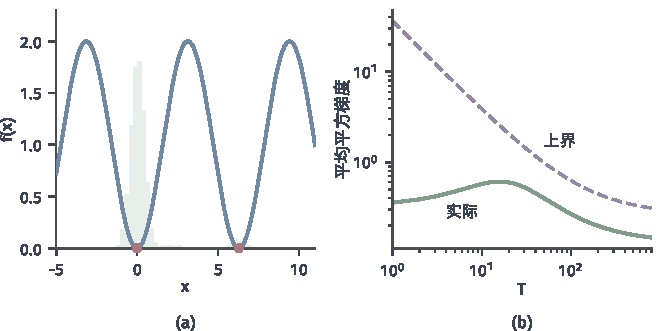
\includegraphics[width=112mm]{figures/05-optimization/05-stochastic-optimization/matplotlib/sgd-nonconvex-output/figure.pdf}
  \caption{非凸目标$f(x)=1-\cos x$上$6000$次独立运行的随机梯度方法（种子固定），$x^{(0)}=2.5$，$\alpha=0.1$。(a)蓝线是目标函数，红点是最小点$x=0$和$2\pi$，绿底直方图是$T=800$时按权重随机返回的点的分布（纵向已缩放）。(b)绿线是$T$步内平方梯度的平均，紫色虚线是式~\eqref{eq:sgd-nonconvex-bound}的上界，两轴取对数。}
  \label{fig:sgd-nonconvex-output}
\end{BookInlineFigure}

图~\ref{fig:sgd-nonconvex-output}(b)显示实际平均约为$0.147$，低于上界$0.312$。上界的第二项$\alpha L\sigma^2$对应的正是噪声底，这个上界在$T$增大时不趋于零，要趋于零必须同时缩小$\alpha$。图(a)中大多数返回点集中在$x=0$附近，少数越过山峰到了$2\pi$附近。

\paragraph{这个结论不说明什么}
式~\eqref{eq:sgd-nonconvex-bound}只评价一阶驻定。小梯度的点可能在鞍点或平坦的高处，它与局部极小的距离没有被保证；能否离开鞍点是第~\ref{chap:saddle-points}章的主题。

它也是期望界，不是逐路径保证。由Markov不等式，对$\varepsilon>0$，
\[
 \mathbb{P}\bigl(\lVert\nabla f(\bm{x}^{(\tau)})\rVert_2^2\geq\varepsilon\bigr)\leq\frac{\mathbb{E}[\lVert\nabla f(\bm{x}^{(\tau)})\rVert_2^2]}{\varepsilon},
\]
只给出一次运行的概率控制。随着$t\to\infty$路径本身的行为，例如几乎处处收敛，需要鞅收敛等工具，可参考\BookChapterRef{chap:discrete-time-stochastic-processes}{卷九第3章“离散时间随机过程”}。

\subsection{随机邻近梯度}
\label{sec:sgd-proximal}

目标带非光滑项时，上面的更新不能直接用。本小节要解决的问题是：非光滑项确定而光滑项需要抽样，邻近步该怎样接上随机读数？

\paragraph{主要思想}
设复合目标$F(\bm{x})=f(\bm{x})+h(\bm{x})$，其中$f$是光滑的有限和或期望目标，$h$是适当、下半连续的凸函数，且邻近映射可以计算。\term{随机邻近梯度法}（stochastic proximal gradient method）只对光滑部分抽样，$h$则每步精确处理：
\begin{equation}
 \bm{x}^{(t+1)}=\operatorname{prox}_{\alpha^{(t)}h}\bigl(\bm{x}^{(t)}-\alpha^{(t)}\hat{\bm{g}}^{(t)}\bigr),
 \label{eq:sgd-prox-update}
\end{equation}
其中邻近映射的定义和计算见第~\ref{chap:nonsmooth-composite-optimization}章。$h$不参与抽样，只在邻近步中出现，这样$\hat{\bm{g}}^{(t)}$的条件无偏性只关系到$f$。

\paragraph{计算过程}
在三项目标上加$h(x)=\gamma\lvert x\rvert$，取$\gamma=1$。复合目标的最优解满足$2x-2+\gamma=0$，所以$x^\star=0.5$，它是正的，与$\lvert x\rvert$的导数取$+1$相符。邻近映射是软阈值：
\[
 \operatorname{prox}_{\alpha h}(z)=\operatorname{sign}(z)\max\{\lvert z\rvert-\alpha\gamma,0\}.
\]
变量与第~\ref{sec:sgd-basic}小节相同，多一个非光滑项的参数。每轮更新三步：抽样下标$i^{(t)}$，走一步随机梯度得到中间点$\bm{z}^{(t)}$，求$\bm{z}^{(t)}$的邻近点作为$\bm{x}^{(t+1)}$。

例中取$x^{(t)}=0.2$，$\alpha=0.1$，阈值是$0.1$。三项读数分别是$3.2,0.4,-8.4$，完整梯度是$-1.6$。走完梯度步的三种结果是
\[
 z=-0.12,\quad z=0.16,\quad z=1.04,
\]
对应的邻近点分别是
\[
 -0.02,\quad 0.06,\quad 0.94.
\]

\paragraph{随机更新的均值不等于精确更新}
三个邻近点的平均是$0.327$。精确更新则先平均梯度，$z=0.36$，邻近点是$0.26$。两者不相等。

\begin{BookInlineFigure}
  \centering
  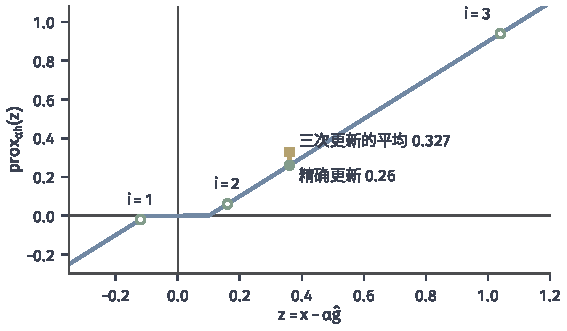
\includegraphics[width=96mm]{figures/05-optimization/05-stochastic-optimization/matplotlib/sgd-prox-bias/figure.pdf}
  \caption{邻近映射的非线性。蓝线是阈值为$0.1$的软阈值函数。三个空心点是三种读数对应的结果。实心绿点是先平均$z$再求邻近点的精确更新，黄方块是三次邻近点的平均。两点之差来自软阈值在零附近的弯折。}
  \label{fig:sgd-prox-bias}
\end{BookInlineFigure}

图~\ref{fig:sgd-prox-bias}说明了原因：邻近映射是非线性的，先平均再映射与先映射再平均结果不同。所以即使$\hat{\bm{g}}^{(t)}$条件无偏，随机更新的均值一般也不等于精确更新。这就是不能直接沿用无偏分析的地方。

\paragraph{误差的评价}
凸情形用复合目标差评价。证明的关键是引入精确更新点，把含噪声的内积拆开。

\begin{theorem}[随机邻近梯度的平均点]
\label{thm:sgd-prox}
设$f$凸且梯度$L$-Lipschitz，$h$适当、下半连续、凸，$F=f+h$有最小点$\bm{x}^\star$。读数条件无偏，沿迭代点$\sigma_t^2\leq\sigma^2$，固定步长$0<\alpha\leq1/L$。记$R=\lVert\bm{x}^{(0)}-\bm{x}^\star\rVert_2$，$\bar{\bm{x}}^{(T)}$为$\bm{x}^{(1)},\ldots,\bm{x}^{(T)}$的算术平均，则
\begin{equation}
 \mathbb{E}[F(\bar{\bm{x}}^{(T)})]-F(\bm{x}^\star)\leq\frac{R^2}{2\alpha T}+\alpha\sigma^2.
 \label{eq:sgd-prox-bound}
\end{equation}
\end{theorem}

\begin{proof}
证明中把当前点和下一点记为$\bm{x},\bm{x}^+$，噪声记为$\bm{\zeta}$，比较点$\bm{u}$取为$\bm{x}^\star$。由下降引理和$f$的凸性，
\[
 f(\bm{x}^+)\leq f(\bm{u})+\langle\nabla f(\bm{x}),\bm{x}^+-\bm{u}\rangle+\frac{L}{2}\lVert\bm{x}^+-\bm{x}\rVert_2^2.
\]

邻近点的最优性条件说明$(\bm{x}-\alpha\hat{\bm{g}}^{(t)}-\bm{x}^+)/\alpha$是$h$在$\bm{x}^+$处的次梯度，于是
\[
 h(\bm{x}^+)\leq h(\bm{u})-\langle\hat{\bm{g}}^{(t)},\bm{x}^+-\bm{u}\rangle+\frac{1}{\alpha}\langle\bm{x}-\bm{x}^+,\bm{x}^+-\bm{u}\rangle.
\]

把两式相加。对最后的内积使用恒等式
\[
 2\langle\bm{x}-\bm{x}^+,\bm{x}^+-\bm{u}\rangle=\lVert\bm{x}-\bm{u}\rVert_2^2-\lVert\bm{x}^+-\bm{u}\rVert_2^2-\lVert\bm{x}^+-\bm{x}\rVert_2^2.
\]
由$\alpha\leq1/L$，$\lVert\bm{x}^+-\bm{x}\rVert_2^2$的系数$L/2-1/(2\alpha)$非正，可以丢掉，得到
\[
 F(\bm{x}^+)-F(\bm{u})\leq\frac{\lVert\bm{x}-\bm{u}\rVert_2^2-\lVert\bm{x}^+-\bm{u}\rVert_2^2}{2\alpha}-\langle\bm{\zeta},\bm{x}^+-\bm{u}\rangle.
\]

最后一项里$\bm{x}^+$依赖$\bm{\zeta}$，条件期望不为零。这里引入用真梯度算出的精确更新点
\[
 \bm{p}=\operatorname{prox}_{\alpha h}\bigl(\bm{x}-\alpha\nabla f(\bm{x})\bigr).
\]
它由历史确定，于是
\[
 \mathbb{E}[\langle\bm{\zeta},\bm{p}-\bm{u}\rangle\mid\mathcal{F}^{(t)}]=0.
\]

邻近映射是非扩张的，两个输入相差$\alpha\bm{\zeta}$，所以$\bm{x}^+$与$\bm{p}$的距离不超过$\alpha\lVert\bm{\zeta}\rVert_2$。再由Cauchy--Schwarz不等式，
\[
 -\langle\bm{\zeta},\bm{x}^+-\bm{p}\rangle\leq\alpha\lVert\bm{\zeta}\rVert_2^2.
\]

取条件期望，得到
\[
 \mathbb{E}[F(\bm{x}^+)\mid\mathcal{F}^{(t)}]-F(\bm{u})\leq\frac{\lVert\bm{x}-\bm{u}\rVert_2^2-\mathbb{E}[\lVert\bm{x}^+-\bm{u}\rVert_2^2\mid\mathcal{F}^{(t)}]}{2\alpha}+\alpha\sigma^2.
\]
取全期望后对$t=0,\ldots,T-1$求和，距离项逐项相消，再除以$T$，并由$F$的凸性用Jensen不等式，即得式~\eqref{eq:sgd-prox-bound}。
\end{proof}

非凸的光滑部分要用另一种度量。精确邻近梯度映射是
\begin{equation}
 \bm{G}_\alpha(\bm{x})=\frac{1}{\alpha}\Bigl[\bm{x}-\operatorname{prox}_{\alpha h}\bigl(\bm{x}-\alpha\nabla f(\bm{x})\bigr)\Bigr],
 \label{eq:sgd-prox-mapping}
\end{equation}
$\bm{G}_\alpha(\bm{x})=\bm{0}$恰好是复合目标的驻点条件。把$\nabla f$换成读数就得到含噪声的读数，它不能代替驻点残差。例中$x=0.2$处$G_\alpha=(0.2-0.26)/0.1=-0.6$，而三次含噪读数是$2.2$，$1.4$，$-7.4$，平均$-1.27$，既不等于$-0.6$，也没有哪一次接近它。这种读数变小，不能说明当前点接近驻点。

\subsection{随机块更新}
\label{sec:sgd-block}

第~\ref{chap:block-optimization}章的分块方法每步只更新变量的一块。本节的方法每步只读一部分目标项。两者可以同时使用，这时要说清每种随机选择各带来什么。

\paragraph{两种随机选择}
把变量分成$J$块，第$j$块的偏梯度记为$\nabla_jf$，$\bm{U}_j$把第$j$块的向量放回全长向量的相应位置，其余分量补零。随机块更新在第$t$步选一块$j^{(t)}$，抽一项$i^{(t)}$，然后
\begin{equation}
 \bm{x}^{(t+1)}=\bm{x}^{(t)}-\alpha_{j^{(t)}}\bm{U}_{j^{(t)}}\nabla_{j^{(t)}}f_{i^{(t)}}(\bm{x}^{(t)}).
 \label{eq:sgd-block-update}
\end{equation}
选块是对变量抽样，选项是对目标项抽样，图~\ref{fig:sgd-block-item-grid}用一张二维表表示。

\begin{BookInlineFigure}
  \centering
  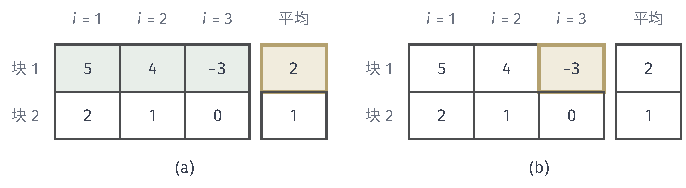
\includegraphics[width=112mm]{figures/05-optimization/05-stochastic-optimization/tikz/sgd-block-item-grid/figure.pdf}
  \caption{读取一次的范围。行是变量块，列是目标项，表中数字是第$i$项对第$j$块的偏导。(a)只随机选块：读完一行所有项（绿底），得到精确的偏梯度（黄框）。(b)同时选块和选项：只读一格（黄框），这个数是偏导的一次读数。}
  \label{fig:sgd-block-item-grid}
\end{BookInlineFigure}

用二元的例子把数字写出来。把贯穿例的$x$记作$x_1$，再加一个变量$x_2$，令第$i$项是
\[
 f_i(x_1,x_2)=\frac{a_i}{2}(x_1-b_i)^2+\frac12(x_2-c_i)^2,\qquad(c_1,c_2,c_3)=(-1,0,1).
\]
在$(2,1)$处，第一块的三个偏导是$5,4,-3$，平均$2$；第二块的三个偏导是$2,1,0$，平均$1$。

\paragraph{固定历史后的核对}
分两层取条件期望。先固定历史和选中的块$j$，只对目标项求平均，由式~\eqref{eq:sgd-uniform-mean}得到
\[
 \mathbb{E}\bigl[\nabla_jf_{i^{(t)}}(\bm{x}^{(t)})\mid\mathcal{F}^{(t)},j\bigr]=\nabla_jf(\bm{x}^{(t)}).
\]
所以给定块之后读数对这一块的偏梯度无偏，条件方差记为$\sigma_j^2$。这一条要求选项的抽样分布不依赖于这一步的读数。若先把各块的读数算出来，再选读数最大的块，结果就有偏。

对选中的块使用块光滑常数$L_j$，第~\ref{chap:block-optimization}章的块下降引理给出的单步界与式~\eqref{eq:sgd-one-step}同样推导：
\begin{equation}
 \begin{aligned}
 \mathbb{E}[f(\bm{x}^{(t+1)})\mid\mathcal{F}^{(t)},j]
 \leq{}&f(\bm{x}^{(t)})-\alpha_j\Bigl(1-\frac{L_j\alpha_j}{2}\Bigr)\lVert\nabla_jf(\bm{x}^{(t)})\rVert_2^2\\
 &+\frac{L_j\alpha_j^2}{2}\sigma_j^2.
 \end{aligned}
 \label{eq:sgd-block-one-step}
\end{equation}

\paragraph{两类随机性并存时}
再对块的选择求平均。取块均匀，$\alpha_j=1/L_j$，由式~\eqref{eq:sgd-block-one-step}，
\[
 \mathbb{E}[f(\bm{x}^{(t+1)})\mid\mathcal{F}^{(t)}]\leq f(\bm{x}^{(t)})-\frac{1}{J}\sum_{j=1}^{J}\frac{\lVert\nabla_jf(\bm{x}^{(t)})\rVert_2^2}{2L_j}+\frac{1}{J}\sum_{j=1}^{J}\frac{\sigma_j^2}{2L_j}.
\]
只随机选块时$\sigma_j=0$，退回第~\ref{chap:block-optimization}章的结论，读取一行的成本是$N$项对这一块的偏导。同时抽样时，一次更新只读一格，代价小得多，但多出噪声项，邻域和步长都要像上面那样处理。

步长也要按两种随机性分别考虑：块步长$\alpha_j$由块光滑常数决定，抽样噪声则要求更小的步长或方差控制。一个容易犯的错误是把噪声项算成所有块的方差之和，而每次其实只读一块；另一个错误是只对选项取期望，忘记选块也是随机的。例中在$(2,1)$处，选块均匀、$\alpha_j=0.1$时，平均更新量是
\[
 -\frac12\cdot0.1\cdot(2,1)=(-0.1,-0.05).
\]
这是两层平均的结果：选中第一块时第一个分量的平均更新是$-0.2$，第二个分量不变，第二块反过来。一次实际抽样中，比如选第一块、第三项，更新量是$(+0.3,0)$，这与平均方向相反，与第~\ref{sec:sgd-unbiased}小节的单项读数相反的情形相同。

\section{方差控制}
\label{sec:sgd-variance}

上一节的误差界都有一项与噪声方差$\sigma^2$成正比。目标和精度要求固定时，把这一项压下去就能用更少的更新达到相同的结果。有哪些办法减小读数的方差，每种办法又要付出多少读取、存储和维护成本？这两件事必须一起看，方差减小不等于总计算减少。

三类办法依次是：一次多读几项，改变抽项的分布，利用已经读过的梯度。

\subsection{小批量与梯度累积}
\label{sec:sgd-minibatch}

\paragraph{批量平均的方差}
最直接的办法是一次读$B$项取平均。设给定历史后$\hat{\bm{g}}_1,\ldots,\hat{\bm{g}}_B$独立同分布，且都是$\nabla f(\bm{x})$的无偏读数，条件方差为$\sigma^2$。\term{小批量}（mini-batch）读数是
\begin{equation}
 \hat{\bm{g}}_{(B)}=\frac{1}{B}\sum_{k=1}^{B}\hat{\bm{g}}_k.
 \label{eq:sgd-minibatch}
\end{equation}

记$\bm{\zeta}_k=\hat{\bm{g}}_k-\nabla f(\bm{x})$。把平方展开，分成平方项和交叉项：
\[
 \mathbb{E}\Bigl[\Bigl\lVert\frac{1}{B}\sum_{k}\bm{\zeta}_k\Bigr\rVert_2^2\;\Big|\;\mathcal{F}^{(t)}\Bigr]
 =\frac{1}{B^2}\sum_{k}\mathbb{E}[\lVert\bm{\zeta}_k\rVert_2^2\mid\mathcal{F}^{(t)}]+\frac{1}{B^2}\sum_{k\neq l}\mathbb{E}[\langle\bm{\zeta}_k,\bm{\zeta}_l\rangle\mid\mathcal{F}^{(t)}].
\]

给定历史时$\bm{\zeta}_k$和$\bm{\zeta}_l$独立且条件均值为零，所以内积的条件期望等于两个条件均值的内积，即零。平方项一共$B$个，所以
\begin{equation}
 \operatorname{Var}\bigl[\hat{\bm{g}}_{(B)}\mid\mathcal{F}^{(t)}\bigr]=\frac{\sigma^2}{B}.
 \label{eq:sgd-minibatch-variance}
\end{equation}
关键在于交叉项消失，这是独立带来的。若读数之间相关，交叉项不再为零，须把它们的协方差保留在展开式中。

\paragraph{无放回的方差}
从$N$项中无放回地抽$B$项，读数不独立，交叉项有确定的值。记$\bm{v}_i=\nabla f_i(\bm{x})-\nabla f(\bm{x})$，它们的和是零，平均平方是$\sigma^2$。对$\lVert\sum_i\bm{v}_i\rVert_2^2=0$展开，得到
\[
 \sum_{i}\lVert\bm{v}_i\rVert_2^2+\sum_{i\neq j}\langle\bm{v}_i,\bm{v}_j\rangle=0.
\]
所以不同的两项的内积平均是$-\sigma^2/(N-1)$。

把这个值代入上面的展开式，交叉项一共$B(B-1)$个，得到
\begin{equation}
 \operatorname{Var}\bigl[\hat{\bm{g}}_{(B)}\mid\mathcal{F}^{(t)}\bigr]=\frac{\sigma^2}{B}\cdot\frac{N-B}{N-1}.
 \label{eq:sgd-minibatch-no-replacement}
\end{equation}
因子$(N-B)/(N-1)$小于$1$。$B=N$时方差为零，正是读完全部的情形。

在三项目标的$x^\star$处核对，这时$\sigma^2=56/3$，读数$(4,2,-6)$的和是零。取$B=2$无放回，三种配对的平均读数是$3,\,-1,\,-2$，平方的平均是
\[
 \frac{9+1+4}{3}=\frac{14}{3}.
\]
公式~\eqref{eq:sgd-minibatch-no-replacement}给出同一结果：$\tfrac{56/3}{2}\cdot\tfrac12=\tfrac{14}{3}$。有放回的$B=2$则是$28/3$，多了一倍。

\begin{BookInlineFigure}
  \centering
  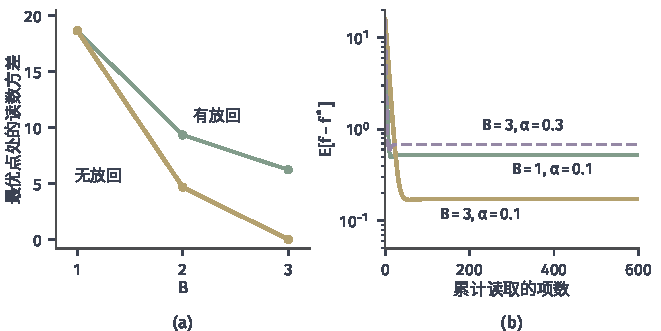
\includegraphics[width=112mm]{figures/05-optimization/05-stochastic-optimization/matplotlib/sgd-minibatch-variance/figure.pdf}
  \caption{小批量的方差与成本，三项目标。(a)最优点处读数方差随批量的变化，绿线有放回，黄线无放回，$B=3$时无放回的方差为零。(b)从$x^{(0)}=5$出发的期望目标差，由精确递推算出，横轴是累计读取的项数。绿线$B=1$，黄线$B=3$且步长相同，紫色虚线$B=3$且步长乘以$3$。}
  \label{fig:sgd-minibatch-variance}
\end{BookInlineFigure}

\paragraph{方差减小不等于计算减少}
式~\eqref{eq:sgd-minibatch-variance}让噪声项除以$B$，但读取量乘以$B$。图~\ref{fig:sgd-minibatch-variance}(b)说明了两者的权衡。步长不变时，$B=3$的噪声底从$0.53$降到$0.17$；把步长也放大$3$倍，保持每次读取走过的距离不变，$B=3$的噪声底是$0.68$，并不比$B=1$更好，初始阶段的下降也差不多。在步长可以随批量调整的范围内，增加批量和缩小步长的效果大体相同，总读取量并没有节省。

增加批量的价值在别处：多个读数可以并行计算，矩阵运算可以成批进行，方差小了也允许使用更稳健的步长。这些是实现上的收益，须按实际硬件单独计算。

\paragraph{梯度累积}
批量太大、一次放不进内存时，可以把它拆成若干微批量，分别算梯度后加起来，只更新一次，这称为\term{梯度累积}（gradient accumulation）。设批量$B$拆成微批量，大小为$n_1,\ldots,n_K$，$\sum_kn_k=B$。设第$k$个微批量的平均读数为$\hat{\bm{g}}_k$，累积时必须按样本数加权：
\begin{equation}
 \hat{\bm{g}}_{(B)}=\sum_{k=1}^{K}\frac{n_k}{B}\hat{\bm{g}}_k.
 \label{eq:sgd-accumulation}
\end{equation}

\begin{BookInlineFigure}
  \centering
  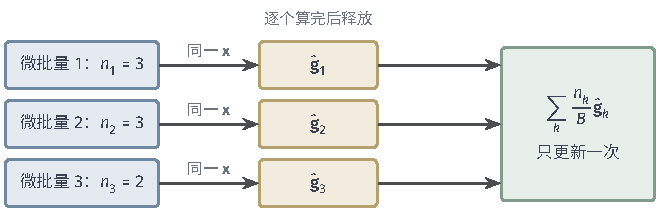
\includegraphics[width=112mm]{figures/05-optimization/05-stochastic-optimization/tikz/sgd-gradient-accumulation/figure.pdf}
  \caption{梯度累积。批量$8$拆成大小为$3,3,2$的微批量。参数在整个过程中保持不变，每个微批量的梯度算完就可以释放它占用的样本与中间结果。累积时按$n_k/B$加权，全部读完后才更新一次。}
  \label{fig:sgd-gradient-accumulation}
\end{BookInlineFigure}

图~\ref{fig:sgd-gradient-accumulation}显示了三个要求。第一，整个累积过程中参数$\bm{x}$不变，否则各微批量的梯度算在不同的点上，加起来不是一个点的梯度。第二，目标函数不变，包括确定的正则项只加一次。第三，权重按样本数计。三项目标上把第一、二项作为一个微批量，第三项单独作为一个，$x=2$处
\[
 \frac23\cdot\frac{5+4}{2}+\frac13\cdot(-3)=2,
\]
与三项的平均相同。若不加权，直接平均两个微批量的读数，得到$(4.5-3)/2=0.75$，答案错了。

读数若还依赖批内统计量，例如用批内均值做归一化，拆开后微批量的统计量与整批不同，累积结果不再等于整批的结果，这些统计量要在整批范围内统一更新。

梯度累积减少的只是同时占用的存储，总读取量仍是$B$。它不是一种降低方差的新办法，只是用更长的时间换更少的内存，方差与整批相同。

\subsection{非均匀抽样}
\label{sec:sgd-importance}

有些项的梯度大，有些小。均匀抽样对所有项一视同仁，把更多机会给“重要”的项，能否减小方差？

\paragraph{逆概率权重}
以固定的正概率$p_1,\ldots,p_N$抽项，$\sum_ip_i=1$。为使条件均值仍是完整梯度，要给读数加上逆概率权重：
\begin{equation}
 \hat{\bm{g}}=\frac{1}{Np_i}\nabla f_i(\bm{x})+\nabla r(\bm{x}).
 \label{eq:sgd-importance-estimator}
\end{equation}
确定的正则梯度$\nabla r$无需抽样，单独加入。条件均值按概率加权直接计算，分母上的$p_i$与概率相消：
\[
 \sum_{i=1}^{N}p_i\cdot\frac{1}{Np_i}\nabla f_i(\bm{x})+\nabla r(\bm{x})=\frac{1}{N}\sum_{i=1}^{N}\nabla f_i(\bm{x})+\nabla r(\bm{x}).
\]
这就是式~\eqref{eq:sgd-finite-sum-regularized}的完整梯度。这种做法称为\term{非均匀抽样}（non-uniform sampling），权重也称重要性权重。

权重不能省略。第~\ref{sec:sgd-unbiased}小节的概率$(1/2,1/4,1/4)$在不加权时，实际被最小化的是加权目标$\tfrac12f_1+\tfrac14f_2+\tfrac14f_3$，它的梯度是
\[
 \frac12(x+3)+\frac14\cdot2x+\frac14(3x-9)=\frac74x-\frac34.
\]
零点是$x=3/7$，而不是$x^\star=1$。算法的不动点取决于读数的条件均值，而不取决于更新的形式。

\paragraph{不同概率下的二阶矩}
无偏之后比较方差，只需比较二阶矩，因为均值已固定。设$r=0$，读数$\tfrac{1}{Np_i}\nabla f_i$的二阶矩是
\begin{equation}
 M(\bm{p})=\sum_{i=1}^{N}p_i\Bigl\lVert\frac{\nabla f_i(\bm{x})}{Np_i}\Bigr\rVert_2^2=\frac{1}{N^2}\sum_{i=1}^{N}\frac{\lVert\nabla f_i(\bm{x})\rVert_2^2}{p_i}.
 \label{eq:sgd-importance-second-moment}
\end{equation}

由Cauchy--Schwarz不等式，
\[
 \Bigl(\sum_i\lVert\nabla f_i\rVert_2\Bigr)^2\leq\Bigl(\sum_i\frac{\lVert\nabla f_i\rVert_2^2}{p_i}\Bigr)\Bigl(\sum_ip_i\Bigr).
\]
于是$M(\bm{p})$的最小值是$(\sum_i\lVert\nabla f_i\rVert_2)^2/N^2$，在$p_i\propto\lVert\nabla f_i(\bm{x})\rVert_2$时取到。最优概率依赖当前点，而算出它需要读完全部的项，这与抽样的目的相矛盾。

在三项目标的$x^\star$处，读数是$(4,2,-6)$，代入式~\eqref{eq:sgd-importance-second-moment}比较三种概率：
\[
 \begin{aligned}
 \bm{p}=\bigl(\tfrac13,\tfrac13,\tfrac13\bigr):\quad&M=\tfrac{56}{3}\approx18.67,\\
 \bm{p}\propto(L_1,L_2,L_3)=\bigl(\tfrac16,\tfrac13,\tfrac12\bigr):\quad&M=20,\\
 \bm{p}\propto(\lvert4\rvert,\lvert2\rvert,\lvert{-6}\rvert)=\bigl(\tfrac13,\tfrac16,\tfrac12\bigr):\quad&M=16.
 \end{aligned}
\]
常用的$p_i\propto L_i$在这个点上比均匀更差。这种选择有另外的好处：加权后各项的光滑常数$L_i/(Np_i)$相同，都等于$\bar{L}=\tfrac1N\sum_iL_i=2$，而不再是$L_{\max}=3$。依赖逐项光滑常数的步长上界因此放宽。

\begin{BookInlineFigure}
  \centering
  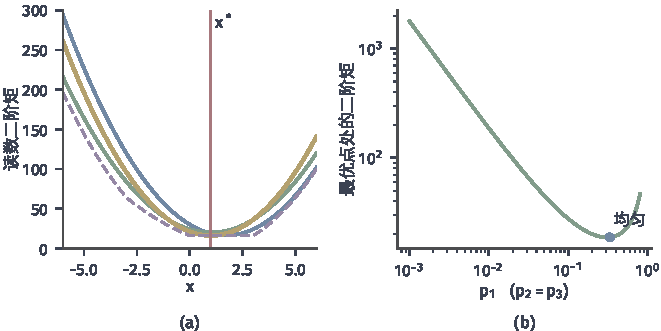
\includegraphics[width=112mm]{figures/05-optimization/05-stochastic-optimization/matplotlib/sgd-importance-sampling/figure.pdf}
  \caption{非均匀抽样的二阶矩，三项目标。(a)不同固定概率下的读数二阶矩随$x$的变化：蓝线均匀，绿线$p_i\propto L_i$，黄线$p_i\propto\lvert f_i'(x^\star)\rvert$，紫色虚线是每点都用最优概率的下包络，红线是$x^\star$。(b)最优点处二阶矩随$p_1$的变化，$p_2=p_3=(1-p_1)/2$，两轴取对数，蓝点是均匀抽样。}
  \label{fig:sgd-importance-sampling}
\end{BookInlineFigure}

图~\ref{fig:sgd-importance-sampling}(a)显示，三条曲线在不同位置各有胜负。没有哪个固定的分布处处最好，这是最优概率依赖$\bm{x}$的直接表现。图(b)说明另一个危险：概率过小会放大读数。$p_1=0.01$时第一项读数被放大$1/(3\cdot0.01)\approx33$倍，$x^\star$处的二阶矩升到约$187$，是均匀抽样的十倍。一项只要可能有非零梯度，就要给它不太小的概率。

代价方面要算三笔账。计算概率需要各项的$L_i$或梯度范数的估计；维护离散分布、每次抽样需要合适的数据结构，概率更新后还要维护；若各项尺度相近，这些投入得不到回报。只有各项差异明显、概率容易得到时，非均匀抽样才值得使用。

\subsection{SVRG}
\label{sec:sgd-svrg}

小批量靠多读减小方差，方差只能按$1/B$下降，到最优点也不消失。有没有办法让读数的方差随迭代点靠近解而自动趋于零？图~\ref{fig:sgd-term-gradients}(b)的观察给出了线索：三条单项导数虽然不同，但都是光滑变化的，在相邻两点的差别不大。

\paragraph{主要思想}
控制变量的想法是：如果要估计一个数，手里还有一个与它高度相关且均值已知的量，就可以用它来纠偏。这里的已知量是一个旧点的梯度。

选一个快照点$\tilde{\bm{x}}$，事先计算好它的完整梯度$\nabla f(\tilde{\bm{x}})$。此后每一步抽$i$，用同一项在当前点和快照点的梯度差，加上快照的完整梯度：
\begin{equation}
 \hat{\bm{g}}=\nabla f_i(\bm{x})-\nabla f_i(\tilde{\bm{x}})+\nabla f(\tilde{\bm{x}}).
 \label{eq:sgd-svrg-direction}
\end{equation}
这就是\term{SVRG}（stochastic variance reduced gradient）\scite{johnson2013accelerating}的方向。$\nabla f_i(\tilde{\bm{x}})$称为\term{控制变量}（control variate）。

对$i$求条件平均，第一项是$\nabla f(\bm{x})$，后两项相消：
\[
 \mathbb{E}[\hat{\bm{g}}\mid\mathcal{F}^{(t)}]=\nabla f(\bm{x})-\nabla f(\tilde{\bm{x}})+\nabla f(\tilde{\bm{x}})=\nabla f(\bm{x}).
\]
所以$\hat{\bm{g}}$条件无偏，这里不需要任何关于$\tilde{\bm{x}}$的假设。方差却取决于$\bm{x}$和$\tilde{\bm{x}}$的距离：若$\bm{x}=\tilde{\bm{x}}$，$\hat{\bm{g}}$恰为完整梯度，一点噪声也没有。

三项目标的读数是一次函数，修正后的方向很简单：
\[
 \hat{g}=a_i(x-\tilde{x})+f'(\tilde{x}).
\]

\begin{BookInlineFigure}
  \centering
  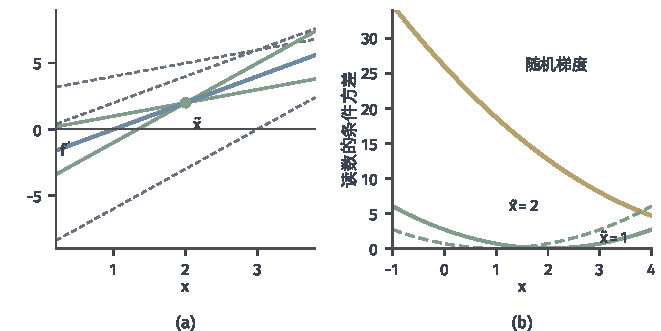
\includegraphics[width=112mm]{figures/05-optimization/05-stochastic-optimization/matplotlib/sgd-svrg-fan/figure.pdf}
  \caption{SVRG的纠偏，三项目标，快照$\tilde{x}=2$。(a)虚线是原始的三项读数，绿线是修正后的读数，蓝线是$f'$。修正后的三条线都经过快照处的点$(2,f'(2))$。(b)读数的条件方差随$x$的变化：黄线是普通随机梯度，绿实线是快照$\tilde{x}=2$，绿虚线是快照$\tilde{x}=1=x^\star$。}
  \label{fig:sgd-svrg-fan}
\end{BookInlineFigure}

图~\ref{fig:sgd-svrg-fan}(a)说明了修正的几何含义：原始的三条读数线各自散开，修正后都绕着快照处的完整梯度旋转，$x$越接近快照，分散越小。条件方差的表达式是$\tfrac23(x-\tilde{x})^2$，它在$x=\tilde{x}$处为零，这正是图(b)的绿线。比较$x=1$这一点，快照$\tilde{x}=2$时条件方差是$2/3$，普通随机梯度是$56/3$。

快照要不断更新。随着$\bm{x}$收敛，把快照移过来，图(b)的绿线就从实线变成虚线，方差在解处变成零。这样，算法每隔若干步要花一次完整梯度的成本重新设置快照，因此有内外两层循环，如图~\ref{fig:sgd-svrg-loop}所示。

\begin{BookInlineFigure}
  \centering
  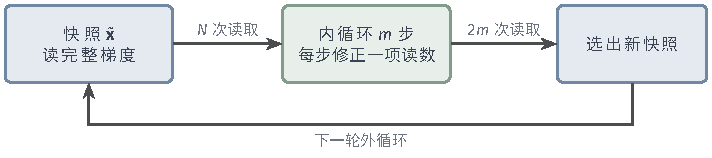
\includegraphics[width=110mm]{figures/05-optimization/05-stochastic-optimization/tikz/sgd-svrg-loop/figure.pdf}
  \caption{SVRG的两层循环。外循环计算完整梯度（$N$次读取）并存下快照，内循环运行$m$步，每步用式~\eqref{eq:sgd-svrg-direction}，读取同一项在两点的梯度（$2$次读取）。一轮外循环共$N+2m$次读取。}
  \label{fig:sgd-svrg-loop}
\end{BookInlineFigure}

\needspace{6\baselineskip}
\paragraph{变量}
\begin{itemize}
 \item $\tilde{\bm{x}}\in\mathbb{R}^n$：快照点。
 \item $\tilde{\bm{g}}\in\mathbb{R}^n$：快照点的完整梯度$\nabla f(\tilde{\bm{x}})$。
 \item $\bm{x}^{(t)}\in\mathbb{R}^n$：内循环的当前点，$t=0,\ldots,m$。
 \item $\alpha>0$，$m$：步长和内循环长度。
\end{itemize}

\paragraph{初始化}
取初始快照$\tilde{\bm{x}}$。例中取$\tilde{x}=2$，$\alpha=0.05$，这满足后面定理的条件，由式~\eqref{eq:sgd-example-gradients}，
\[
 \tilde{g}=f'(2)=2.
\]

\paragraph{每轮更新}
外循环的一轮按下列步骤进行。

\begin{enumerate}
 \item 快照：置$\bm{x}^{(0)}=\tilde{\bm{x}}$，计算$\tilde{\bm{g}}=\nabla f(\tilde{\bm{x}})$，共$N$次读取。例中$x^{(0)}=2$，$\tilde{g}=2$。
 \item 内循环：对$t=0,\ldots,m-1$，抽下标$i^{(t)}$，按式~\eqref{eq:sgd-svrg-direction}得到方向$\hat{\bm{g}}^{(t)}$，沿它走步长$\alpha$得到新点。

 例中第一步抽到$i=3$，$x^{(0)}=\tilde{x}$，方向就是完整梯度，
 \[
  \hat{g}^{(0)}=2,\qquad x^{(1)}=2-0.05\cdot2=1.9.
 \]

 第二步抽到$i=1$，$a_1=1$，方向和新点是
 \[
  \hat{g}^{(1)}=1\cdot(1.9-2)+2=1.9,\qquad x^{(2)}=1.9-0.05\cdot1.9=1.805.
 \]

 第三步抽到$i=2$，$a_2=2$，方向和新点是
 \[
  \hat{g}^{(2)}=2\cdot(1.805-2)+2=1.61,\qquad x^{(3)}=1.805-0.05\cdot1.61=1.7245.
 \]
 \item 选取新快照：从内循环的点中选一个作为新的$\tilde{\bm{x}}$。下面的定理要求在$\bm{x}^{(0)},\ldots,\bm{x}^{(m-1)}$中均匀随机选取，实践中也常取最后一点。
\end{enumerate}

外循环达到预定轮数后结束。最终得到最后一次的快照。例中三步都朝$x^\star=1$靠近，方向全部为正，没有再出现单项读数$-3$带来的上坡，这正是控制变量的效果。

\paragraph{差分的方差与收敛}
证明方差自动减小的关键，是用目标差控制逐项梯度的差。需要假设每一项都是光滑的凸函数。

\begin{lemma}[逐项梯度差的控制]
\label{lem:sgd-gradient-difference}
设$f_i$凸且梯度$L$-Lipschitz，$f=\frac1N\sum_if_i$有最小点$\bm{x}^\star$。则对任意$\bm{x}$，
\begin{equation}
 \frac{1}{N}\sum_{i=1}^{N}\lVert\nabla f_i(\bm{x})-\nabla f_i(\bm{x}^\star)\rVert_2^2\leq2L\bigl(f(\bm{x})-f^\star\bigr).
 \label{eq:sgd-gradient-difference}
\end{equation}
\end{lemma}

\begin{proof}
定义
\[
 \psi_i(\bm{x})=f_i(\bm{x})-f_i(\bm{x}^\star)-\langle\nabla f_i(\bm{x}^\star),\bm{x}-\bm{x}^\star\rangle.
\]
$\psi_i$凸，梯度$L$-Lipschitz，$\nabla\psi_i(\bm{x}^\star)=\bm{0}$，所以$\bm{x}^\star$是它的最小点，最小值为$0$。

对$\psi_i$从$\bm{x}$走一步$\bm{x}-\nabla\psi_i(\bm{x})/L$，由下降引理，
\[
 0\leq\psi_i\Bigl(\bm{x}-\frac{1}{L}\nabla\psi_i(\bm{x})\Bigr)\leq\psi_i(\bm{x})-\frac{1}{2L}\lVert\nabla\psi_i(\bm{x})\rVert_2^2.
\]

$\nabla\psi_i(\bm{x})$就是$\nabla f_i(\bm{x})$与$\nabla f_i(\bm{x}^\star)$的差。对$i$平均时，由$\nabla f(\bm{x}^\star)=\bm{0}$，一次项消失，$\psi_i$的平均恰为$f(\bm{x})-f^\star$。整理即得式~\eqref{eq:sgd-gradient-difference}。
\end{proof}

\begin{theorem}[SVRG的线性收缩]
\label{thm:sgd-svrg}
设每个$f_i$凸且梯度$L$-Lipschitz，$f$是$\mu$强凸的。设$0<\alpha<1/(4L)$，$m$足够大，使
\begin{equation}
 \rho=\frac{1}{\mu\alpha(1-2L\alpha)m}+\frac{2L\alpha}{1-2L\alpha}<1.
 \label{eq:sgd-svrg-rate}
\end{equation}
每轮外循环的新快照在$\bm{x}^{(0)},\ldots,\bm{x}^{(m-1)}$中均匀随机选取。则相邻两轮的快照$\tilde{\bm{x}}_{s}$，$\tilde{\bm{x}}_{s+1}$满足
\begin{equation}
 \mathbb{E}[f(\tilde{\bm{x}}_{s+1})]-f^\star\leq\rho\bigl(\mathbb{E}[f(\tilde{\bm{x}}_s)]-f^\star\bigr).
 \label{eq:sgd-svrg-contraction}
\end{equation}
\end{theorem}

\begin{proof}
固定一轮外循环，$\tilde{\bm{x}}$由此前的历史确定。记$\bm{x}=\bm{x}^{(t)}$，$E_x=f(\bm{x})-f^\star$，$E_s=f(\tilde{\bm{x}})-f^\star$。先控制方向的二阶矩。

在方向~\eqref{eq:sgd-svrg-direction}中加减$\nabla f_i(\bm{x}^\star)$，把它写成两段之和，再用不等式$(a+b)^2\leq2a^2+2b^2$，得到
\[
 \lVert\hat{\bm{g}}\rVert_2^2\leq2\lVert\nabla f_i(\bm{x})-\nabla f_i(\bm{x}^\star)\rVert_2^2+2\lVert\nabla f_i(\tilde{\bm{x}})-\nabla f_i(\bm{x}^\star)-\nabla f(\tilde{\bm{x}})\rVert_2^2.
\]

第二段里，$\nabla f_i(\tilde{\bm{x}})-\nabla f_i(\bm{x}^\star)$的条件均值恰为$\nabla f(\tilde{\bm{x}})$，第二段就是它减去自己的均值。方差不超过二阶矩，所以去掉$\nabla f(\tilde{\bm{x}})$后条件期望不会变小。对两段分别用式~\eqref{eq:sgd-gradient-difference}，得到
\[
 \mathbb{E}[\lVert\hat{\bm{g}}\rVert_2^2\mid\mathcal{F}^{(t)}]\leq4L(E_x+E_s).
\]

再展开距离。由条件无偏和$f$的凸性，内积项不小于$E_x$，于是
\[
 \mathbb{E}[\lVert\bm{x}^{(t+1)}-\bm{x}^\star\rVert_2^2\mid\mathcal{F}^{(t)}]\leq\lVert\bm{x}-\bm{x}^\star\rVert_2^2-2\alpha E_x+4L\alpha^2(E_x+E_s).
\]

对$t=0,\ldots,m-1$求和取全期望，距离项相消，并丢掉非负的终点距离。记$\bar{E}$为内循环点目标差的平均，它也是随机选出的新快照的期望目标差，得到
\[
 2\alpha(1-2L\alpha)m\bar{E}\leq\mathbb{E}\lVert\tilde{\bm{x}}-\bm{x}^\star\rVert_2^2+4L\alpha^2m\mathbb{E}[E_s].
\]

强凸性给出快照点的距离上界$\tfrac{2}{\mu}E_s$，代入后得到
\[
 2\alpha(1-2L\alpha)m\bar{E}\leq\Bigl(\frac{2}{\mu}+4L\alpha^2m\Bigr)\mathbb{E}[E_s].
\]
两边除以$2\alpha(1-2L\alpha)m$，即得式~\eqref{eq:sgd-svrg-contraction}。
\end{proof}

式~\eqref{eq:sgd-svrg-rate}的两项分别表示：内循环够长，初始距离的影响才能被摊薄；步长够小，快照带来的方差项才小于收缩。这里$L$是单项的光滑常数，在三项目标上$L=3$，$\mu=2$。取$\alpha=0.05<1/12$，$m=50$，得到
\[
 \rho=\frac{1}{2\cdot0.05\cdot0.7\cdot50}+\frac{0.3}{0.7}\approx0.286+0.429=0.714.
\]
这是一个保守的上界。三项目标从$\tilde{x}=2$开始一轮的实际结果，用$20000$次独立运行的平均来估计，目标差约从$1$降到$0.115$。

\paragraph{成本}
一轮外循环需要$N+2m$次读取，每轮把目标差减小一个固定比例。取$\alpha$为$1/L$的小常数倍、$m$与$\kappa$同量级时$\rho$是小于$1$的常数，所以减小一个固定比例约需$N+\kappa$量级的读取，这里$\kappa=L/\mu$用单项的光滑常数计算。完整梯度下降减小同样的比例约需$N\kappa_f$量级的读取，其中$\kappa_f$用$f$本身的光滑常数计算。$N$很大时前者优势明显。存储上，SVRG只保存$\tilde{\bm{x}}$和$\tilde{\bm{g}}$两个向量，每步重新计算$\nabla f_i(\tilde{\bm{x}})$。也可以事先保存所有项的快照梯度，每步只需一次读取，但内存要多$N$个向量。内循环长度$m$、快照的频率，在理论和实践之间常有差别，定理的$m$往往偏大。

SVRG要求能重复访问所有项，且每轮要算一次完整梯度，所以只适用于有限和目标；样本源源不断的期望目标不能直接用。

\subsection{SAGA}
\label{sec:sgd-saga}

SVRG要定期花一次完整梯度来设置快照。如果把每一项上次读到的梯度都记下来，是不是不用专门做快照，靠记忆逐步更新就够了？这就是SAGA\scite{defazio2014saga}的想法。

\paragraph{主要思想}
为每一项维护一个存下的旧梯度$\bm{\phi}_i$，以及它们的均值$\bar{\bm{\phi}}=\frac1N\sum_i\bm{\phi}_i$。每一步抽$i$，用新读数减去这一项的旧读数，再加上旧均值：
\begin{equation}
 \hat{\bm{g}}=\nabla f_i(\bm{x})-\bm{\phi}_i+\bar{\bm{\phi}}.
 \label{eq:sgd-saga-direction}
\end{equation}
这与SVRG的方向形式相同，只是把快照点的梯度换成了各项自己记录的旧梯度。给定历史，表项都是确定的，对$i$求条件平均，第二、三项相消，所以方向条件无偏。

完成参数更新之后，才把表项$\bm{\phi}_i$替换成新读数，并同步修改均值：
\begin{equation}
 \bar{\bm{\phi}}\leftarrow\bar{\bm{\phi}}+\frac{1}{N}\bigl(\nabla f_i(\bm{x})-\bm{\phi}_i\bigr).
 \label{eq:sgd-saga-mean}
\end{equation}
这个次序不能交换。若先把$\bm{\phi}_i$换成新读数，方向就变成$\bar{\bm{\phi}}$，只是旧梯度的平均，新读数根本没有进入更新，条件无偏也失去了。

\needspace{6\baselineskip}
\paragraph{变量}
\begin{itemize}
 \item $\bm{x}^{(t)}\in\mathbb{R}^n$：当前点。
 \item $\bm{\phi}_i\in\mathbb{R}^n$，$i=1,\ldots,N$：各项记录的旧梯度，共$N$个向量。
 \item $\bar{\bm{\phi}}\in\mathbb{R}^n$：表项的均值，用式~\eqref{eq:sgd-saga-mean}增量更新，不必每次重算。
 \item $\alpha>0$：步长。
\end{itemize}

\paragraph{初始化}
在初始点读全部$N$项填满梯度表，$N$次读取。例中取$x^{(0)}=2$，$\alpha=0.05$，表项和均值是
\[
 (\phi_1,\phi_2,\phi_3)=(5,4,-3),\qquad \bar{\phi}=2.
\]

\paragraph{每轮更新}
对$t=0,1,\ldots$依次执行以下步骤。

\begin{enumerate}
 \item 抽样并读取：抽$i^{(t)}$，计算新读数$\nabla f_{i^{(t)}}(\bm{x}^{(t)})$，这是一次读取。例中第一轮抽到$i=3$，新读数是$-3$。
 \item 计算方向并更新：由式~\eqref{eq:sgd-saga-direction}，例中第一轮
 \[
  \hat{g}^{(0)}=-3-(-3)+2=2,\qquad x^{(1)}=2-0.05\cdot2=1.9.
 \]
 \item 更新表项：把$\bm{\phi}_{i^{(t)}}$换成新读数，按式~\eqref{eq:sgd-saga-mean}修改均值。例中第一轮新读数与旧表项相同，$\phi_3$和均值都不变。
\end{enumerate}

例中第二轮抽到$i=1$，新读数$f_1'(1.9)=4.9$，方向和新点是
\[
 \hat{g}^{(1)}=4.9-5+2=1.9,\qquad x^{(2)}=1.9-0.05\cdot1.9=1.805.
\]
然后$\phi_1$变成$4.9$，均值变成$(4.9+4-3)/3\approx1.967$。

例中第三轮抽到$i=2$，新读数$f_2'(1.805)=3.61$，方向和新点是
\[
 \hat{g}^{(2)}\approx3.61-4+1.967=1.577,\qquad x^{(3)}\approx1.805-0.05\cdot1.577=1.726.
\]
然后$\phi_2$变成$3.61$，均值变成$(4.9+3.61-3)/3\approx1.837$。图~\ref{fig:sgd-saga-table}画出了表的变化。

\begin{BookInlineFigure}
  \centering
  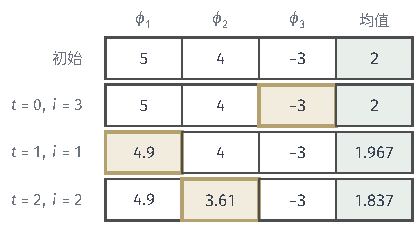
\includegraphics[width=72mm]{figures/05-optimization/05-stochastic-optimization/tikz/sgd-saga-table/figure.pdf}
  \caption{SAGA的梯度表在三步内的变化。每行是完成该步之后的表，黄框是刚被替换的项，右列是表的均值。第一步新读数恰好等于旧表项，表不变；此后只有被抽到的项发生变化。}
  \label{fig:sgd-saga-table}
\end{BookInlineFigure}

迭代在读取量达到预定预算后结束，最终得到$\bm{x}^{(T)}$；例中三步后$x^{(3)}\approx1.726$，每步一次读取，加上初始化的三次，共六次读取。

\paragraph{两种误差共同评价}
SAGA的状态比普通方法多一张表，所以进展要同时看两件事：参数离解多远，表项离各自的$\nabla f_i(\bm{x}^\star)$多远。参数接近解之后，表项还可能很旧，方差还不会小。要让方差趋于零，就需要每一项都被更新到解附近。

\begin{theorem}[SAGA的线性收敛]
\label{thm:sgd-saga}
设每个$f_i$凸且梯度$L$-Lipschitz，$f$是$\mu$强凸的，取$\alpha=1/(3L)$，下标独立均匀抽取，梯度表在初始点填满。则存在只依赖初始距离和初始表项误差的常数$C$，使
\begin{equation}
 \mathbb{E}[\lVert\bm{x}^{(T)}-\bm{x}^\star\rVert_2^2]\leq\Bigl(1-\min\Bigl\{\frac{1}{4N},\frac{\mu}{3L}\Bigr\}\Bigr)^TC.
 \label{eq:sgd-saga-rate}
\end{equation}
\end{theorem}

式~\eqref{eq:sgd-saga-rate}的证明需要构造一个同时包含距离和各表项误差的函数，并证明它的期望按上述比例收缩，推导较长，读者可查阅原始论文\scite{defazio2014saga}。这里解释结论的机制。速率的最小值中有两项：$\mu/(3L)$与单纯的梯度下降类似，由条件数决定；$1/(4N)$反映表项的刷新速度，每一步只刷新一项，刷新一遍大约需要$N$步。$N$很大时，记忆更新是瓶颈，反过来则是条件数决定收敛。

在三项目标上，$N=3$，$L=3$，$\mu=2$，所以
\[
 \min\Bigl\{\frac{1}{12},\frac29\Bigr\}=\frac{1}{12},
\]
定理保证的是每步收缩$11/12$。手算所用的$\alpha=0.05$小于$1/(3L)=1/9$，只用来演示表项的变化。

SAGA没有强凸性时也有保证，平均点的目标差按$1/T$的量级下降，常数与$N$有关，这里不再讨论。

\paragraph{比较}
表~\ref{tab:sgd-vr-compare}按读取和存储比较这些方法。方差控制的共同代价是：多读或多存，并依赖逐项光滑、凸性等结构。

\begin{BookInlineTable}
  \centering
  \begin{tabular}{llll}
    \toprule
    方法 & 每次更新读取 & 存储 & 需要重复访问\\
    \midrule
    随机梯度 & $1$ & $1$个向量 & 否\\
    小批量 & $B$ & $1$个向量 & 否\\
    SVRG & $2$，另有每轮$N$ & $2$个向量 & 是\\
    SAGA & $1$，初始化$N$ & $N+2$个向量 & 是\\
    \bottomrule
  \end{tabular}
  \caption{方差控制方法的成本。存储只计迭代所需向量，随机梯度和小批量含当前点。}
  \label{tab:sgd-vr-compare}
\end{BookInlineTable}

SAGA的表要存$N$个$n$维向量，这在$N$和$n$都很大时是沉重的负担。对各项梯度是某个数乘已知向量的线性模型，每个表项只需存一个标量，才算切实可行。

图~\ref{fig:sgd-vr-cost}用一个$N=500$、$n=20$的正则最小二乘实例比较总读取量。横轴是读取量除以$N$，即完整遍历的轮数。随机梯度初期最快，但很快到达噪声底。完整梯度稳定下降，但每步代价是$N$。SVRG和SAGA在初期略慢于随机梯度，此后保持线性收敛，目标差继续下降到比噪声底小许多个量级的水平。

\begin{BookInlineFigure}
  \centering
  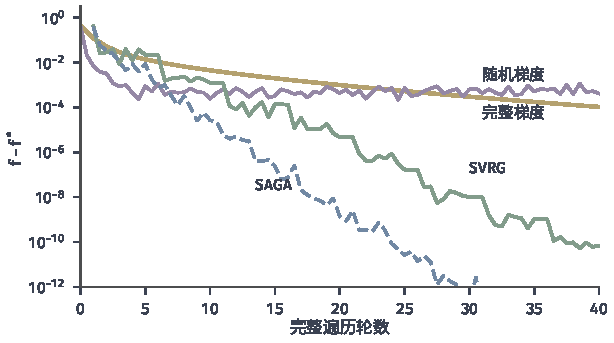
\includegraphics[width=104mm]{figures/05-optimization/05-stochastic-optimization/matplotlib/sgd-vr-cost/figure.pdf}
  \caption{总读取量与目标差，$N=500$、$n=20$的正则最小二乘实例（种子固定），$\lVert\bm{a}_i\rVert_2=1$，$\gamma=0.005$。黄线是完整梯度，紫线是固定步长$0.1$的随机梯度，绿线是SVRG（$\alpha=0.2/L$，$m=2N$，此处$L$取单项的光滑常数），蓝色虚线是SAGA（$\alpha=1/(3L)$）。横轴是读取量除以$N$，纵轴取对数。}
  \label{fig:sgd-vr-cost}
\end{BookInlineFigure}

这个比较的结论有边界：只针对这一个实例和这一组参数，SVRG和SAGA的优势在需要高精度时才明显。若只需低精度，或者问题本身的噪声底已经够用，普通随机梯度加小批量更简单；若数据是流式的，不能重复访问，这两种方法都用不上。

\section{随机动量方法}
\label{sec:sgdb-momentum}

小批量和控制变量都在改善单步的读数，代价是多读梯度或多存梯度。本节换一个问题：不增加读取，只把已经读过的梯度组合进当前方向，能得到什么，又要付出什么？

组合历史读数有两种效果。一致的成分累积起来，随机涨落互相抵消，这是平滑；旧读数来自旧的位置，当前梯度变化时方向跟不上，这是滞后。两者同时发生，而且历史进入了算法的状态，每一步的误差要连同历史一起分析。本节先讲当前点读数的重球法，再讲前瞻点读数的Nesterov方法，最后讲两种把动量做非线性变换的方法。

\subsection{随机重球法}
\label{sec:sgdb-heavy-ball}

\paragraph{主要思想}
第~\ref{chap:first-order-methods}章的重球法在当前梯度步之外，再加上一步历史位移。把其中的梯度换成当前点的随机读数$\hat{\bm g}^{(t)}$，就得到\term{随机重球法}（stochastic heavy ball method）。规定$\bm{x}^{(-1)}=\bm{x}^{(0)}$，
\begin{equation}
 \bm{x}^{(t+1)}=\bm{x}^{(t)}-\alpha\hat{\bm g}^{(t)}+\beta\bigl(\bm{x}^{(t)}-\bm{x}^{(t-1)}\bigr),\qquad 0\leq\beta<1.
 \label{eq:sgdb-hb}
\end{equation}

式~\eqref{eq:sgdb-hb}要存两个位置。实际计算常改写成只存一个速度向量$\bm{v}^{(t)}$的形式：取$\bm{v}^{(0)}=\bm{0}$，先更新速度，再更新位置，
\begin{equation}
 \bm{v}^{(t+1)}=\beta\bm{v}^{(t)}+\hat{\bm g}^{(t)},\qquad
 \bm{x}^{(t+1)}=\bm{x}^{(t)}-\alpha\bm{v}^{(t+1)}.
 \label{eq:sgdb-hb-velocity}
\end{equation}

两种写法等价。由速度形式，上一步的位移满足$\bm{x}^{(t)}-\bm{x}^{(t-1)}=-\alpha\bm{v}^{(t)}$，于是
\[
 -\alpha\bm{v}^{(t+1)}=-\alpha\hat{\bm g}^{(t)}-\alpha\beta\bm{v}^{(t)}
 =-\alpha\hat{\bm g}^{(t)}+\beta\bigl(\bm{x}^{(t)}-\bm{x}^{(t-1)}\bigr).
\]

还有第三种常见写法，把方向写成读数的移动平均。令$\bm{m}^{(t)}=(1-\beta)\bm{v}^{(t)}$，式~\eqref{eq:sgdb-hb-velocity}的速度递推两边乘以$1-\beta$，得到
\begin{equation}
 \bm{m}^{(t+1)}=\beta\bm{m}^{(t)}+(1-\beta)\hat{\bm g}^{(t)},\qquad
 \bm{x}^{(t+1)}=\bm{x}^{(t)}-\alpha'\bm{m}^{(t+1)},
 \label{eq:sgdb-hb-ema}
\end{equation}
其中两种写法的步长的对应关系是
\begin{equation}
 \alpha'=\frac{\alpha}{1-\beta}.
 \label{eq:sgdb-hb-effective}
\end{equation}

对应关系决定了调参的含义。在速度写法中固定$\alpha$而增大$\beta$，方向的总权重变大，$\alpha/(1-\beta)$随之变大，所以$\alpha/(1-\beta)$称为\term{有效步长}（effective step size）。在移动平均写法中固定$\alpha'$而增大$\beta$，方向的总权重不变，只是平均的窗口更长。比较两种实现时，先把参数换到同一种写法。

\paragraph{历史权重：平滑与滞后}
方向怎样由历史读数组成？反复代入速度递推，得到
\begin{equation}
 \bm{v}^{(t+1)}=\sum_{s=0}^{t}\beta^{t-s}\hat{\bm g}^{(s)}.
 \label{eq:sgdb-hb-weights}
\end{equation}

一个$s$轮之前的读数，权重是$\beta^{s}$，按等比衰减。移动平均写法中的权重是$(1-\beta)\beta^{s}$，全部加起来等于$1-\beta^{t+1}$，轮数足够多时接近$1$。图~\ref{fig:sgdb-momentum-track}(a)画出两个$\beta$对应的权重：$\beta$越接近$1$，权重越平，记忆越长。

\begin{BookInlineFigure}
  \centering
  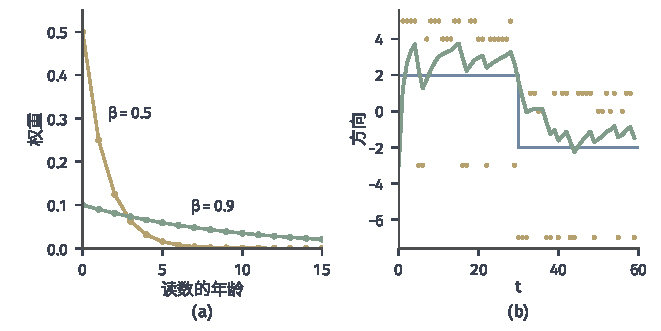
\includegraphics[width=112mm]{figures/05-optimization/05-stochastic-optimization/matplotlib/sgdb-momentum-track/figure.pdf}
  \caption{移动平均的平滑与滞后。(a)读数按年龄的权重$(1-\beta)\beta^{s}$，黄线$\beta=0.5$，绿线$\beta=0.9$。(b)蓝线是真实梯度，在$t=30$由$2$突变为$-2$；黄点是加上贯穿例噪声后的单次读数；绿线是$\beta=0.9$的移动平均方向（按权重之和归一化）。绿线的抖动比黄点小得多，但突变后要约十轮才转向。}
  \label{fig:sgdb-momentum-track}
\end{BookInlineFigure}

把两种效果算出来。先看平滑：设各轮读数的噪声相互独立，方差都是$\sigma^2$。移动平均的噪声部分是加权和，独立项的方差按权重平方相加，
\[
 (1-\beta)^2\sum_{s=0}^{t}\beta^{2s}\,\sigma^2
 =\frac{1-\beta}{1+\beta}\bigl(1-\beta^{2(t+1)}\bigr)\sigma^2 .
\]
于是轮数足够多时，方差缩小的倍数是
\begin{equation}
 \frac{1-\beta}{1+\beta}.
 \label{eq:sgdb-ema-noise}
\end{equation}

再看滞后：移动平均里读数的平均年龄是
\begin{equation}
 \sum_{s=0}^{\infty}s(1-\beta)\beta^{s}=\frac{\beta}{1-\beta}.
 \label{eq:sgdb-ema-age}
\end{equation}

取$\beta=0.9$，噪声方差缩小到约$0.053$倍，平均年龄却是$9$轮。图~\ref{fig:sgdb-momentum-track}(b)同时展示了两者：梯度不变时绿线紧贴真实值，梯度突变后绿线要约十轮才转向。这两个计算都假定噪声与位置无关，只说明趋势：真实运行中读数的位置本身受过去的噪声影响。

\paragraph{动量不是当前梯度的无偏估计}
读数条件无偏是说，固定历史后读数的均值等于当前梯度。动量方向并不继承这个性质。历史$\mathcal{F}^{(t)}$确定了$\bm{v}^{(t)}$，所以
\begin{equation}
 \mathbb{E}\bigl[\bm{v}^{(t+1)}\mid\mathcal{F}^{(t)}\bigr]=\beta\bm{v}^{(t)}+\bm{g}^{(t)},
 \label{eq:sgdb-hb-cond}
\end{equation}
只要$\bm{v}^{(t)}\neq\bm{0}$且$\beta>0$，它就不等于当前梯度$\bm{g}^{(t)}$。移动平均写法同样如此，条件均值是$\beta\bm{m}^{(t)}+(1-\beta)\bm{g}^{(t)}$。前面基于条件无偏的单步下降递推，不能把$\bm{v}^{(t+1)}$当成读数直接代入。

贯穿例给出具体的数。取$\alpha=0.1$，$\beta=0.5$，第一轮抽到第$3$项后位于$x^{(1)}=2.3$，速度是$v^{(1)}=-3$。此时三项梯度分别是$5.3,4.6,-2.1$，平均为$f'(2.3)=2.6$。第二轮的速度取$3.8$、$3.1$、$-3.6$三个值，条件均值是
\[
 \mathbb{E}\bigl[v^{(2)}\mid\mathcal{F}^{(1)}\bigr]=0.5\cdot(-3)+2.6=1.1\neq2.6.
\]

\paragraph{固定噪声下的稳态方差}
动量究竟能不能降低噪声的影响？在可以精确计算的情形中回答。考虑一元二次目标、加性噪声，下面的定理给出重球法长期的方差。

\begin{theorem}[加性噪声下重球法的稳态方差]
\label{thm:sgdb-hb-variance}
设$f(x)=\frac\lambda2x^2$，$\lambda>0$，读数为$\hat g^{(t)}=\lambda x^{(t)}+\xi^{(t)}$，其中$\xi^{(t)}$独立同分布，均值为零，方差为$\sigma^2$，且与此前的迭代独立。设$0\leq\beta<1$，$0<\alpha\lambda<2(1+\beta)$。则式~\eqref{eq:sgdb-hb}的迭代满足$\mathbb{E}x^{(t)}\to0$，并且
\begin{equation}
 \lim_{t\to\infty}\mathbb{E}\bigl[(x^{(t)})^2\bigr]
 =\frac{\alpha\sigma^2(1+\beta)}{\lambda(1-\beta)\bigl(2(1+\beta)-\alpha\lambda\bigr)}.
 \label{eq:sgdb-hb-variance}
\end{equation}
\end{theorem}

\begin{proof}
把式~\eqref{eq:sgdb-hb}写成二阶递推。令$a_1=1+\beta-\alpha\lambda$，$a_2=-\beta$，$s^2=\alpha^2\sigma^2$，则
\[
 x^{(t+1)}=a_1x^{(t)}+a_2x^{(t-1)}-\alpha\xi^{(t)}.
\]

特征方程是$r^2-a_1r-a_2=0$。条件$0\leq\beta<1$与$\lvert a_1\rvert<1+\beta$合起来保证两根都在单位圆内，这正是定理对$\alpha$和$\beta$的要求。所以均值的线性递推趋于零；二阶矩的线性递推的特征值是两根的两两乘积，也都在单位圆内，因而二阶矩收敛。记极限为
\[
 V_0=\lim_{t\to\infty}\mathbb{E}\bigl[(x^{(t)})^2\bigr],\qquad
 V_1=\lim_{t\to\infty}\mathbb{E}\bigl[x^{(t)}x^{(t-1)}\bigr].
\]

递推两边乘以$x^{(t)}$取期望。$\xi^{(t)}$与$x^{(t)}$独立且均值为零，噪声项消失；取极限得到$V_1=a_1V_0+a_2V_1$，也就是
\[
 V_1=\frac{a_1V_0}{1-a_2}.
\]

递推两边平方取期望，同样消去交叉项，取极限得到
\[
 V_0=(a_1^2+a_2^2)V_0+2a_1a_2V_1+s^2 .
\]

把$V_1$代入，两边乘以$1-a_2$并整理，$V_0$的系数变成
\[
 (1-a_2)(1-a_2^2)-a_1^2(1-a_2)-2a_1^2a_2
 =(1+a_2)\bigl[(1-a_2)^2-a_1^2\bigr].
\]

于是
\[
 V_0=\frac{s^2(1-a_2)}{(1+a_2)\bigl[(1-a_2)^2-a_1^2\bigr]}.
\]

代回$1-a_2=1+\beta$，$1+a_2=1-\beta$，以及
\[
 (1+\beta)^2-(1+\beta-\alpha\lambda)^2=\alpha\lambda\bigl(2(1+\beta)-\alpha\lambda\bigr),
\]
约去一个$\alpha\lambda$，即得式~\eqref{eq:sgdb-hb-variance}。
\end{proof}

看式~\eqref{eq:sgdb-hb-variance}怎样读。取$\beta=0$，它变成常步长随机梯度下降的$\alpha\sigma^2/(\lambda(2-\alpha\lambda))$。当$\alpha\lambda$远小于$1+\beta$时，$2(1+\beta)-\alpha\lambda\approx2(1+\beta)$，稳态方差约为
\begin{equation}
 \frac{\alpha\sigma^2}{2\lambda(1-\beta)}=\frac{\sigma^2}{2\lambda}\cdot\frac{\alpha}{1-\beta},
 \label{eq:sgdb-hb-small-step}
\end{equation}
只取决于有效步长$\alpha/(1-\beta)$。也就是说，步长很小时，动量的平滑效果恰好被有效步长的放大抵消：动量不改变噪声的稳态水平，它带来的是更快的初始收敛。

图~\ref{fig:sgdb-hb-floor}(b)验证了这一点：三个$\beta$的稳态目标差关于有效步长几乎是同一条线。图~\ref{fig:sgdb-hb-floor}(a)回到贯穿例，读数噪声随位置变化，定理的公式不再精确成立，但同样可以写出二阶矩的精确递推。$\alpha=0.1$，$\beta=0.5$的重球法稳态目标差约为$1.037$，有效步长相同的$\alpha=0.2$的随机梯度下降约为$1.217$，$\alpha=0.1$的随机梯度下降约为$0.528$。

\begin{BookInlineFigure}
  \centering
  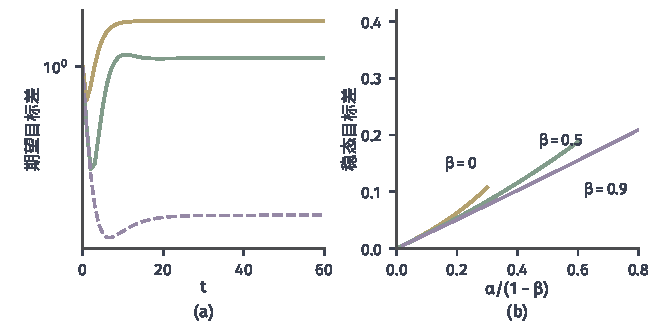
\includegraphics[width=112mm]{figures/05-optimization/05-stochastic-optimization/matplotlib/sgdb-hb-floor/figure.pdf}
  \caption{动量下的噪声残余。(a)贯穿例、$x^{(0)}=2$的期望目标差，由二阶矩的精确递推得到。绿线是$\alpha=0.1$，$\beta=0.5$的重球法；黄线是$\alpha=0.2$的随机梯度下降，有效步长与绿线相同；紫色虚线是$\alpha=0.1$的随机梯度下降。(b)式~\eqref{eq:sgdb-hb-variance}给出的稳态目标差$\frac\lambda2V_0$，$\lambda=2$，$\sigma^2=1$，横轴是有效步长。黄线、绿线、紫线分别取$\beta=0,0.5,0.9$，三条线的$\alpha$都取到$0.3$为止。}
  \label{fig:sgdb-hb-floor}
\end{BookInlineFigure}

\needspace{6\baselineskip}
\paragraph{变量}
\begin{itemize}
 \item $\bm{x}^{(t)}\in\mathbb{R}^n$：当前参数。
 \item $\bm{v}^{(t)}\in\mathbb{R}^n$：速度，形状与参数相同，是算法状态的一部分。
 \item $\hat{\bm g}^{(t)}\in\mathbb{R}^n$：当前点的随机读数。
 \item $\alpha>0$，$0\leq\beta<1$：固定的步长与动量系数。
 \item $T$：预定的总轮数。
\end{itemize}

\paragraph{初始化}
令$\bm{v}^{(0)}=\bm{0}$，第一轮没有历史，与一步随机梯度下降相同。例中是贯穿例的三项一元目标，取$\alpha=0.1$，$\beta=0.5$，读取顺序为第$3,1,2$项，起点和速度是
\[
 x^{(0)}=2,\qquad v^{(0)}=0.
\]

\needspace{6\baselineskip}
\paragraph{每轮更新}
在第$t$轮依次执行：
\begin{enumerate}
 \item \textbf{抽样并读取。}抽取下标$i^{(t)}$，在当前点读取$\hat{\bm g}^{(t)}$。这一步使用的是更新前的位置。例中第一轮抽到第$3$项，
 \[
  \hat g^{(0)}=f_3'(2)=-3.
 \]
 \item \textbf{更新速度。}按式~\eqref{eq:sgdb-hb-velocity}用旧速度和本轮读数计算$\bm{v}^{(t+1)}$。例中第一轮
 \[
  v^{(1)}=0.5\cdot0+(-3)=-3.
 \]
 \item \textbf{更新参数。}用新速度计算$\bm{x}^{(t+1)}$，然后$t\leftarrow t+1$。例中第一轮
 \[
  x^{(1)}=2-0.1\cdot(-3)=2.3.
 \]

 第二轮抽到第$1$项，读数和速度是
 \[
  \hat g^{(1)}=f_1'(2.3)=5.3,\qquad v^{(2)}=0.5\cdot(-3)+5.3=3.8,
 \]
 于是
 \[
  x^{(2)}=2.3-0.38=1.92.
 \]

 第三轮抽到第$2$项，读数和速度是
 \[
  \hat g^{(2)}=f_2'(1.92)=3.84,\qquad v^{(3)}=0.5\cdot3.8+3.84=5.74,
 \]
 于是
 \[
  x^{(3)}=1.92-0.574=1.346.
 \]
\end{enumerate}

单次读数的大小不能作为停止依据，这里按预定轮数结束。例中$T=3$，最终得到$x^{(3)}=1.346$，目标差为$(0.346)^2\approx0.120$。

\paragraph{保证与状态}
随机重球法每轮只多一个$n$维向量和一次向量加法，读取次数不变。恢复运行时必须同时恢复$\bm{v}^{(t)}$：只恢复参数，第一轮就退回了一步无动量的随机梯度下降。

一般目标上的保证要同时限定$\alpha$、$\beta$和读数的条件。定理~\ref{thm:sgdb-hb-variance}只针对二次目标和加性噪声。第~\ref{chap:first-order-methods}章已经看到，重球法在一般强凸光滑目标上，用二次目标的最优参数可能循环；随机读数不会修复这一点。分析时要把$(\bm{x}^{(t)},\bm{v}^{(t)})$作为一个整体，常用的做法是构造同时包含目标差和速度的势函数，递推中的噪声项按所选的势函数进入。

\subsection{随机Nesterov方法}
\label{sec:sgdb-nesterov}

\paragraph{主要思想}
第~\ref{chap:first-order-methods}章的Nesterov方法先沿动量探出去，到探出的位置再求梯度。随机版本的读数也放到这个前瞻点：
\begin{equation}
 \begin{aligned}
 \bm{y}^{(t)}&=\bm{x}^{(t)}+\beta\bigl(\bm{x}^{(t)}-\bm{x}^{(t-1)}\bigr),\\
 \bm{x}^{(t+1)}&=\bm{y}^{(t)}-\alpha\hat{\bm g}^{(t)},
 \end{aligned}
 \label{eq:sgdb-nag}
\end{equation}
这里$\hat{\bm g}^{(t)}$是在$\bm{y}^{(t)}$处读取的。图~\ref{fig:sgdb-state-order}把两种方法的状态次序并排画出。

\begin{BookInlineFigure}
  \centering
  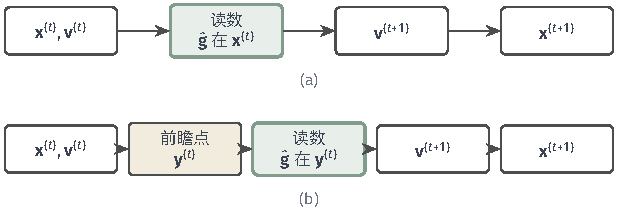
\includegraphics[width=104.64mm]{figures/05-optimization/05-stochastic-optimization/tikz/sgdb-state-order/figure.pdf}
  \caption{一轮内的状态次序。(a)随机重球法在当前点读数，接着更新速度和参数。(b)随机Nesterov方法先用历史算出前瞻点（黄），在前瞻点读数（绿），再更新速度和参数。两种方法的状态都是$(\bm{x}^{(t)},\bm{v}^{(t)})$，读取发生的位置不同。}
  \label{fig:sgdb-state-order}
\end{BookInlineFigure}

$\bm{y}^{(t)}$由抽样之前的量算出，所以固定历史后它是确定的。读数的条件无偏因而写成
\begin{equation}
 \mathbb{E}\bigl[\hat{\bm g}^{(t)}\mid\mathcal{F}^{(t)}\bigr]=\nabla f\bigl(\bm{y}^{(t)}\bigr).
 \label{eq:sgdb-nag-unbiased}
\end{equation}
这里被无偏估计的是前瞻点的梯度，不是$\bm{x}^{(t)}$处的梯度，两者一般不同。下面的比较把这一差别和其他差别列在一起。

\begin{BookInlineTable}
  \centering
  \caption{随机重球法与随机Nesterov方法的比较。}
  \label{tab:sgdb-momentum-compare}
  \begin{tabular}{lll}
    \toprule
    对比项 & 随机重球法 & 随机Nesterov方法\\
    \midrule
    读数位置 & 当前点$\bm{x}^{(t)}$ & 前瞻点$\bm{y}^{(t)}$\\
    条件无偏对象 & $\nabla f(\bm{x}^{(t)})$ & $\nabla f(\bm{y}^{(t)})$\\
    状态 & $\bm{x}^{(t)},\bm{v}^{(t)}$ & $\bm{x}^{(t)},\bm{v}^{(t)}$\\
    一般强凸光滑 & 最优参数可能循环 & 确定性时加速\\
    \bottomrule
  \end{tabular}
\end{BookInlineTable}

贯穿例中取同样的$\alpha=0.1$，$\beta=0.5$，读取顺序仍为第$3,1,2$项。三轮的前瞻点、读数和新位置分别是
\[
 \begin{aligned}
 y^{(0)}&=2, & \hat g^{(0)}&=-3, & x^{(1)}&=2.3,\\
 y^{(1)}&=2.45, & \hat g^{(1)}&=5.45, & x^{(2)}&=1.905,\\
 y^{(2)}&=1.7075, & \hat g^{(2)}&=3.415, & x^{(3)}&=1.366.
 \end{aligned}
\]

第二轮的读数$5.45$是$f_1'$在$y^{(1)}=2.45$处的值，而不是在$x^{(1)}=2.3$处的值。第三轮的前瞻点$1.7075$已经比$x^{(2)}=1.905$更靠近$x^\star=1$，读数相应变小。

\paragraph{方差怎样进入势函数}
确定性的Nesterov方法靠势函数证明加速。把梯度换成带噪声的读数，势函数的递推发生什么变化？下面的定理说明，收缩因子保留，但多了一个不随步数消失的噪声项。记号沿用第~\ref{chap:first-order-methods}章：$q=1/\sqrt\kappa$，以$\bm{u}^{(t)}$表示那里的辅助点。

\begin{theorem}[强凸情形下随机Nesterov方法的势函数递推]
\label{thm:sgdb-nag-noise}
设$f$的梯度$L$-Lipschitz连续且$\mu$强凸，$\mu>0$，最优解为$\bm{x}^\star$。取$\alpha=1/L$，$\beta=(1-q)/(1+q)$，$\bm{x}^{(-1)}=\bm{x}^{(0)}$。设前瞻点的读数满足
\begin{equation}
 \begin{gathered}
 \hat{\bm g}^{(t)}=\nabla f(\bm{y}^{(t)})+\bm{\xi}^{(t)},\\
 \mathbb{E}\bigl[\bm{\xi}^{(t)}\mid\mathcal{F}^{(t)}\bigr]=\bm{0},\qquad
 \mathbb{E}\bigl[\lVert\bm{\xi}^{(t)}\rVert_2^2\mid\mathcal{F}^{(t)}\bigr]\leq\sigma^2.
 \end{gathered}
 \label{eq:sgdb-nag-noise-condition}
\end{equation}
令$\bm{u}^{(0)}=\bm{x}^{(0)}$，并记
\begin{equation}
 \begin{aligned}
 \bm{u}^{(t+1)}&=\bm{x}^{(t)}+\frac1q\bigl(\bm{x}^{(t+1)}-\bm{x}^{(t)}\bigr),\\
 \Phi^{(t)}&=f(\bm{x}^{(t)})-f^\star+\frac\mu2\lVert\bm{u}^{(t)}-\bm{x}^\star\rVert_2^2.
 \end{aligned}
 \label{eq:sgdb-nag-potential}
\end{equation}
则
\begin{equation}
 \mathbb{E}\bigl[\Phi^{(t+1)}\mid\mathcal{F}^{(t)}\bigr]\leq(1-q)\Phi^{(t)}+\frac{\sigma^2}{L},
 \label{eq:sgdb-nag-recursion}
\end{equation}
因而
\begin{equation}
 \mathbb{E}f(\bm{x}^{(T)})-f^\star\leq(1-q)^T\Phi^{(0)}+\frac{\sqrt\kappa\,\sigma^2}{L}.
 \label{eq:sgdb-nag-bound}
\end{equation}
\end{theorem}

\begin{proof}
固定一步，省略上标$(t)$，记$\bm{g}=\nabla f(\bm{y})$，下一步的点记为$\bm{x}^+$和$\bm{u}^+$。

第一步，建立两个恒等式：
\[
 \bm{y}=\frac{\bm{x}+q\bm{u}}{1+q},\qquad
 \bm{u}^+=(1-q)\bm{u}+q\bm{y}-\frac q\mu\hat{\bm g}.
\]
这两个等式只用到更新形式$\bm{x}^+=\bm{y}-\hat{\bm g}/L$，读数是否带噪声不影响代数。第一式在$t=0$时成立，因为$\bm{y}^{(0)}=\bm{u}^{(0)}=\bm{x}^{(0)}$。设第一式对$t$成立，则$q\bm{u}=(1+q)\bm{y}-\bm{x}$，代入第二式右端，并用$q/\mu=1/(qL)$，得到
\[
 \frac1q\bigl(\bm{y}-\tfrac1L\hat{\bm g}-(1-q)\bm{x}\bigr)
 =\bm{x}+\frac1q(\bm{x}^+-\bm{x})=\bm{u}^+ .
\]

再由$\bm{u}^+$的定义和$\beta=(1-q)/(1+q)$，计算
\[
 \frac{\bm{x}^++q\bm{u}^+}{1+q}=\bm{x}^++\frac{1-q}{1+q}(\bm{x}^+-\bm{x})=\bm{y}^{(t+1)},
\]
所以第一式对$t+1$也成立。

第二步，函数项。由下降引理，
\[
 f(\bm{x}^+)\leq f(\bm{y})-\frac1L\langle\bm{g},\hat{\bm g}\rangle+\frac{1}{2L}\lVert\hat{\bm g}\rVert_2^2 .
\]

固定$\mathcal{F}^{(t)}$取条件期望。噪声的条件均值为零，交叉项消失，于是
\[
 \mathbb{E}\hat{\bm g}=\bm{g},\qquad
 \mathbb{E}\lVert\hat{\bm g}\rVert_2^2\leq\lVert\bm{g}\rVert_2^2+\sigma^2 .
\]

代入上式，得到
\[
 \mathbb{E}f(\bm{x}^+)\leq f(\bm{y})-\frac{1}{2L}\lVert\bm{g}\rVert_2^2+\frac{\sigma^2}{2L}.
\]

第三步，距离项。记$\bm{w}=(1-q)\bm{u}+q\bm{y}$，它由历史确定，$\bm{u}^+=\bm{w}-\frac q\mu\hat{\bm g}$。展开平方，用$q^2/(2\mu)=1/(2L)$，取条件期望，得到
\[
 \frac\mu2\mathbb{E}\lVert\bm{u}^+-\bm{x}^\star\rVert_2^2
 \leq\frac\mu2\lVert\bm{w}-\bm{x}^\star\rVert_2^2-q\langle\bm{g},\bm{w}-\bm{x}^\star\rangle+\frac{1}{2L}\bigl(\lVert\bm{g}\rVert_2^2+\sigma^2\bigr).
\]

第四步，相加。两式相加，$\lVert\bm{g}\rVert_2^2$相消，噪声项合计$\sigma^2/L$。剩下的部分完全由历史确定：
\[
 \mathbb{E}\Phi^{(t+1)}\leq f(\bm{y})-f^\star+\frac\mu2\lVert\bm{w}-\bm{x}^\star\rVert_2^2-q\langle\bm{g},\bm{w}-\bm{x}^\star\rangle+\frac{\sigma^2}{L}.
\]

第五步，处理确定部分，与精确梯度时相同。平方范数的凸性给出
\[
 \lVert\bm{w}-\bm{x}^\star\rVert_2^2\leq(1-q)\lVert\bm{u}-\bm{x}^\star\rVert_2^2+q\lVert\bm{y}-\bm{x}^\star\rVert_2^2 .
\]
把$\bm{w}-\bm{x}^\star$写成$(1-q)(\bm{u}-\bm{y})+(\bm{y}-\bm{x}^\star)$，并由强凸性得到
\[
 \langle\bm{g},\bm{y}-\bm{x}^\star\rangle\geq f(\bm{y})-f^\star+\frac\mu2\lVert\bm{y}-\bm{x}^\star\rVert_2^2 .
\]

两式代入后，$\lVert\bm{y}-\bm{x}^\star\rVert_2^2$项抵消，右端成为
\[
 (1-q)\bigl(f(\bm{y})-f^\star\bigr)+(1-q)\frac\mu2\lVert\bm{u}-\bm{x}^\star\rVert_2^2-q(1-q)\langle\bm{g},\bm{u}-\bm{y}\rangle+\frac{\sigma^2}{L}.
\]

第六步，由第一个恒等式，$q(\bm{u}-\bm{y})=\bm{y}-\bm{x}$，所以内积项等于$(1-q)\langle\bm{g},\bm{x}-\bm{y}\rangle$。凸性给出
\[
 \langle\bm{g},\bm{x}-\bm{y}\rangle\leq f(\bm{x})-f(\bm{y}),
\]
于是$f(\bm{y})$消去，得到式~\eqref{eq:sgdb-nag-recursion}。

最后对$t$取全期望并迭代，用$\sum_{j<T}(1-q)^j\leq1/q=\sqrt\kappa$，得到式~\eqref{eq:sgdb-nag-bound}。
\end{proof}

定理的两个条件起不同的作用。条件无偏保证了函数项和距离项中的一次项按精确梯度计算，这是用到式~\eqref{eq:sgdb-nag-noise-condition}第一式的地方。方差界让二次项多出$\sigma^2/(2L)$，函数项和距离项各一份。

与确定性结果的差别在于式~\eqref{eq:sgdb-nag-bound}最后一项。确定性时目标差按$(1-q)^T$收缩到零；有噪声时只能收缩到量级$\sqrt\kappa\sigma^2/L$的邻域，这一项不随$T$消失。所以确定性的加速界不能靠把梯度换成读数直接继承，要进一步下降就要改用更小的步长或增大批量，收缩因子也要随之调整。

式~\eqref{eq:sgdb-nag-bound}是上界，不同方法的上界不宜直接比较。在二次目标上可以写出精确的稳态值。图~\ref{fig:sgdb-accel-noise}用第~\ref{chap:first-order-methods}章的目标$f=(x_1^2+9x_2^2)/2$和起点$(9,1)$比较三种方法。无噪声时，重球法和Nesterov方法远快于梯度下降。加入方差为$1$的加性噪声后，梯度下降、重球法、Nesterov方法的稳态目标差分别约为$0.085$、$0.926$、$0.108$。重球法这组参数的有效步长是$1/3$，大于梯度下降的$1/9$；更重要的是$\lambda=9$时$\alpha\lambda=2.25$，已接近稳定边界$2(1+\beta)=2.5$，式~\eqref{eq:sgdb-hb-variance}的分母很小，噪声残余被放大约$11$倍。Nesterov方法的残余低于定理的上界$\sqrt\kappa\sigma^2/L=1/3$。

\begin{BookInlineFigure}
  \centering
  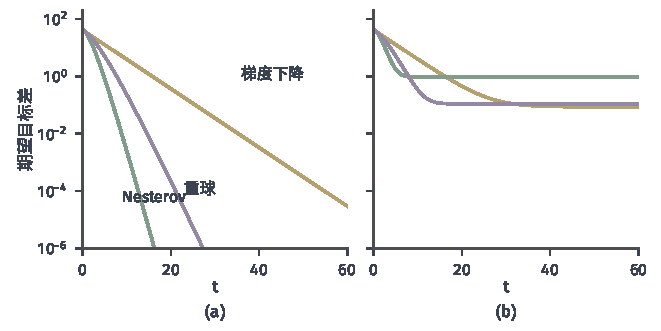
\includegraphics[width=112mm]{figures/05-optimization/05-stochastic-optimization/matplotlib/sgdb-accel-noise/figure.pdf}
  \caption{目标$f=(x_1^2+9x_2^2)/2$，起点$(9,1)$，由二阶矩的精确递推得到的期望目标差。(a)无噪声。(b)读数加上各分量方差为$1$的独立噪声。黄线是$\alpha=1/9$的梯度下降，绿线是$\alpha=\beta=1/4$的重球法，紫线是$\alpha=1/9$，$\beta=1/2$的Nesterov方法。加速缩短了初始阶段，重球法的稳态残余明显更高。}
  \label{fig:sgdb-accel-noise}
\end{BookInlineFigure}

\subsection{Lion符号动量（补充）}
\label{sec:sgdb-lion}

\paragraph{算法}
前两种方法的方向都保留读数的幅度。Lion只取方向的符号：把动量和本轮读数组成候选方向，逐坐标取符号，再按固定步长移动\scite{chen2023lion}。记$\operatorname{sign}(\cdot)$逐坐标作用。取$\bm{m}^{(0)}=\bm{0}$，系数$\beta_1,\beta_2\in[0,1)$，收缩系数$\gamma\geq0$，每轮读取$\hat{\bm g}^{(t)}$后依次计算候选方向和参数更新：
\begin{equation}
 \begin{aligned}
 \bm{c}^{(t)}&=\beta_1\bm{m}^{(t)}+(1-\beta_1)\hat{\bm g}^{(t)},\\
 \bm{x}^{(t+1)}&=\bm{x}^{(t)}-\alpha\operatorname{sign}\bigl(\bm{c}^{(t)}\bigr)-\alpha\gamma\bm{x}^{(t)}.
 \end{aligned}
 \label{eq:sgdb-lion}
\end{equation}

候选方向只参与这一步，下一轮用的动量由另一个系数单独记录：
\begin{equation}
 \bm{m}^{(t+1)}=\beta_2\bm{m}^{(t)}+(1-\beta_2)\hat{\bm g}^{(t)}.
 \label{eq:sgdb-lion-memory}
\end{equation}
$\beta_1$决定当前方向里旧动量占多少，$\beta_2$决定动量本身记忆多长，常见取值是$\beta_1=0.9$，$\beta_2=0.99$。因此读数在方向里的权重是$1-\beta_1$，在历史中的权重却是$1-\beta_2$，两者分开调节。

\paragraph{舍弃幅度}
符号操作舍弃了幅度。设候选方向是$\bm{c}=(0.1,3)$，同向但两个坐标相差$30$倍，取符号后是$(1,1)$，两个坐标移动相同的距离。图~\ref{fig:sgdb-lion-sign}(a)对比了这一点。优点是位移的大小完全由步长决定，读数的尺度和离群值都不会放大位移；缺点是信息少了，当前读数是否接近零，算法并不知道。

\begin{BookInlineFigure}
  \centering
  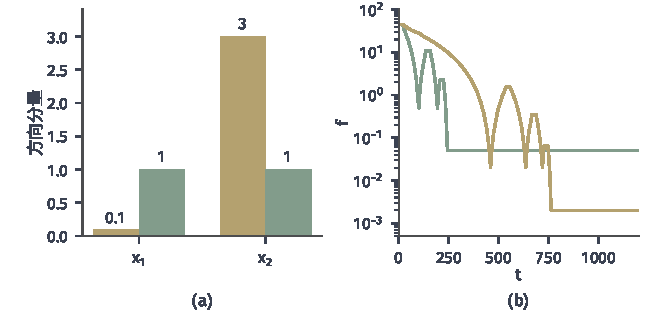
\includegraphics[width=112mm]{figures/05-optimization/05-stochastic-optimization/matplotlib/sgdb-lion-sign/figure.pdf}
  \caption{符号方向的效果。(a)候选方向$(0.1,3)$（黄）与其符号$(1,1)$（绿）。(b)目标$f=(x_1^2+9x_2^2)/2$上$\gamma=0$的Lion，使用精确梯度，纵轴是最近$20$轮内$f$的最大值。绿线$\alpha=0.1$，黄线$\alpha=0.02$。下降段之后曲线不再改善，平台高度随步长变化。}
  \label{fig:sgdb-lion-sign}
\end{BookInlineFigure}

\paragraph{贯穿例的三轮}
取$\alpha=0.1$，$\beta_1=0.9$，$\beta_2=0.99$，$\gamma=0$，$x^{(0)}=2$，$m^{(0)}=0$，读取顺序仍为第$3,1,2$项。三轮的读数、候选方向、新位置和新动量依次是
\[
 \begin{aligned}
 \hat g^{(0)}&=-3, & c^{(0)}&=-0.3, & x^{(1)}&=2.1, & m^{(1)}&=-0.03,\\
 \hat g^{(1)}&=5.1, & c^{(1)}&=0.483, & x^{(2)}&=2.0, & m^{(2)}&=0.0213,\\
 \hat g^{(2)}&=4, & c^{(2)}&=0.419, & x^{(3)}&=1.9, & m^{(3)}&=0.0611.
 \end{aligned}
\]

第一轮的候选方向由反向读数决定，参数上升；此后两轮都下降。读数的大小从$3$变到$5.1$，每轮的位移却都是$0.1$。

\paragraph{分别核对三个量}
第一个量是实际位移：$\gamma=0$时每个坐标的位移大小恰好是$\alpha$（候选方向该坐标非零时），不随读数减小。第二个量是原目标的残差。以$\beta_1=0$的一元精确梯度为例，每步的位移都是$\alpha$，迭代最后在距$x^\star$不超过$\alpha$的范围内来回，残差不会趋于零；$\beta_1>0$时候选方向有滞后，来回的范围由动量决定，同样不会随步数消失。图~\ref{fig:sgdb-lion-sign}(b)取$\beta_1=0.9$，$\beta_2=0.99$，平台的最高值在$\alpha=0.1$时是$0.05$，在$\alpha=0.02$时是$0.002$，减小残差要靠减小步长。

第三个量是参数收缩。$\gamma$项按更新前的参数做收缩，独立于读数和符号。它把参数往原点拉，不是原目标的下降方向，所以残差要按原目标$f$计算，不能把含收缩的位移当成$f$的下降。

\subsection{Muon矩阵动量（补充）}
\label{sec:sgdb-muon}

\paragraph{问题：把矩阵动量变换成更新方向}
参数是矩阵$\bm{W}\in\mathbb{R}^{m\times d}$时，动量$\bm{B}$也是矩阵。Lion逐元素地把幅度抹去，Muon在奇异方向上做类似的事：保留动量的奇异向量，把奇异值全部变成$1$\scite{jordan2024muon}。

这正是极分解所做的。矩形矩阵$\bm{B}$的紧奇异值分解是$\bm{B}=\bm{U}\bm{\Sigma}\bm{V}^\top$，极分解把它写成部分等距与半正定因子之积，
\begin{equation}
 \bm{B}=\bm{U}\bm{V}^\top\cdot\bm{V}\bm{\Sigma}\bm{V}^\top,\qquad
 \operatorname{orth}(\bm{B})=\bm{U}\bm{V}^\top .
 \label{eq:sgdb-polar}
\end{equation}
这里$\bm{U}\bm{V}^\top$就是\term{极因子}（polar factor），奇异向量与$\bm{B}$相同，奇异值全部是$1$。极分解的存在性和唯一性条件可参考\BookChapterRef{chap:polar-decomposition}{卷二第8章“极分解”}。

奇异值分解太贵，Muon用矩阵多项式的有限次迭代来近似极因子。设$\bm{X}=\bm{U}\bm{\Sigma}\bm{V}^\top$，对奇次多项式$p(\sigma)=\sum_jc_j\sigma^{2j+1}$，有
\begin{equation}
 \sum_jc_j\bm{X}\bigl(\bm{X}^\top\bm{X}\bigr)^j=\bm{U}\,p(\bm{\Sigma})\,\bm{V}^\top ,
 \label{eq:sgdb-odd-poly}
\end{equation}
所以这样的迭代不改变奇异向量，只对每个奇异值作用多项式。于是问题变成：选$p$，使得多次复合后所有奇异值都接近$1$。

\paragraph{算法次序}
一次更新的次序是：
\begin{enumerate}
 \item \textbf{读取。}在当前点（或前瞻点）得到矩阵读数$\hat{\bm G}^{(t)}$。
 \item \textbf{更新动量。}用旧动量和本轮读数计算
 \begin{equation}
  \bm{B}^{(t+1)}=\beta\bm{B}^{(t)}+\hat{\bm G}^{(t)}.
  \label{eq:sgdb-muon-momentum}
 \end{equation}
 \item \textbf{归一化。}用Frobenius范数除以动量，得到
 \[
  \bm{X}_0=\frac{\bm{B}^{(t+1)}}{\lVert\bm{B}^{(t+1)}\rVert_{\mathrm{F}}},
 \]
 所有非零奇异值落到$(0,1]$。
 \item \textbf{有限次迭代。}按多项式迭代$k$次，得到$\bm{X}_k$。
 \item \textbf{更新参数。}$\bm{W}^{(t+1)}=\bm{W}^{(t)}-\alpha\bm{X}_k$。
\end{enumerate}

经典的Newton--Schulz迭代取$p(\sigma)=\frac12(3\sigma-\sigma^3)$，矩阵形式是
\begin{equation}
 \bm{X}_{j+1}=\frac32\bm{X}_j-\frac12\bm{X}_j\bm{X}_j^\top\bm{X}_j .
 \label{eq:sgdb-newton-schulz}
\end{equation}
这个$p$有不动点$\sigma=1$，导数$p'(1)=0$，所以在$1$附近二阶收敛；对$\sigma\in(0,1]$迭代单调上升到$1$，起点离零很近时每步只放大约$1.5$倍。归一化保证了奇异值落在收敛区域里。

\paragraph{理想极因子与有限步近似}
用具体矩阵计算。取
\[
 \bm{B}=\begin{bmatrix}3&1\\1&3\end{bmatrix}.
\]
它的奇异值是$4,2$，奇异向量相同，极因子是单位矩阵$\bm{I}$。按Frobenius范数$\sqrt{20}$归一化后，奇异值是
\[
 0.894,\qquad 0.447.
\]

由式~\eqref{eq:sgdb-newton-schulz}迭代一次，两个奇异值变成$0.984$和$0.626$；迭代三次是$1.000$和$0.953$；迭代五次是$1.000$和$0.99998$，已经非常接近理想的极因子$\bm{I}$。图~\ref{fig:sgdb-muon-singular}(a)画出一般的$\sigma$：奇异值越小，需要的迭代次数越多。

\begin{BookInlineFigure}
  \centering
  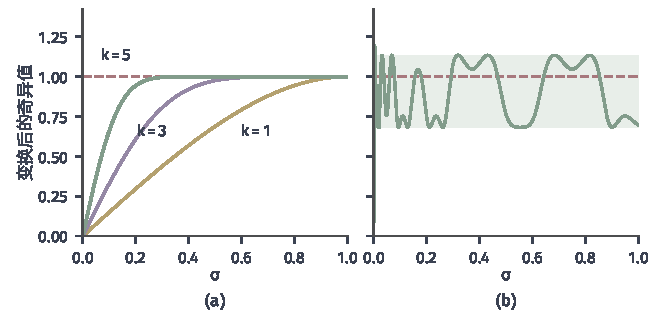
\includegraphics[width=112mm]{figures/05-optimization/05-stochastic-optimization/matplotlib/sgdb-muon-singular/figure.pdf}
  \caption{有限次迭代对奇异值的作用，横轴是归一化后的奇异值，红色虚线是理想的$1$。(a)经典Newton--Schulz迭代$k=1,3,5$次。(b)五次多项式$3.4445\sigma-4.7750\sigma^3+2.0315\sigma^5$复合$5$次，绿底是$\sigma\in[0.02,1]$上的取值范围，约为$[0.68,1.13]$。}
  \label{fig:sgdb-muon-singular}
\end{BookInlineFigure}

实际实现常用五次多项式\scite{jordan2024muon}：
\begin{equation}
 p(\sigma)=3.4445\,\sigma-4.7750\,\sigma^3+2.0315\,\sigma^5 .
 \label{eq:sgdb-muon-poly}
\end{equation}
它的系数是为“只迭代五次”专门选的。$p(1)=0.701$，$\sigma=1$不是它的不动点，继续迭代不会收敛到极因子。它的优势是小奇异值被放大得更快：在图~\ref{fig:sgdb-muon-singular}(b)中，$\sigma\in[0.02,1]$上五次复合后的值都落在约$[0.68,1.13]$内。

上面的矩阵用五次多项式迭代五次，奇异值变成$1.114$和$0.689$，与理想值$1$差得较远；两个奇异值之比从$2$缩小到约$1.6$。所以$\bm{X}_k$是对动量的尺度压缩，而不是精确的极因子。

\paragraph{计算成本与含义}
设$m\geq d$，先把$\bm{X}^\top\bm{X}$算出来。每次迭代做一次$\bm{X}^\top\bm{X}$、一次$(\bm{X}^\top\bm{X})^2$和一次$\bm{X}$右乘，运算量是$O(md^2)$；迭代$k$次合计$O(kmd^2)$。完整的奇异值分解也是这个量级，但常数更大。比较方法时，这部分要计入，每步的读取次数不变不等于每步成本不变。

动量矩阵和它的变换都只由梯度读数算出，其中没有二阶导数。奇异值变成$1$是对历史读数的幅度处理，它不是目标Hessian的近似。这种方法在什么问题上有效，只能在具体问题上由实际的目标值或验证指标判断。

\section{自适应更新}
\label{sec:sgdb-adaptive}

动量决定历史读数怎样合成方向。本节研究历史读数的另一种用途：根据过去读数的幅度，决定每个坐标或每个矩阵方向的更新尺度。不同坐标的读数幅度可能相差几个量级，同一个步长对它们不合适。这些方法都写成
\begin{equation}
 \bm{x}^{(t+1)}=\bm{x}^{(t)}-\alpha^{(t)}\bm{D}^{(t)}\hat{\bm g}^{(t)},
 \label{eq:sgdb-adaptive-form}
\end{equation}
或把$\hat{\bm g}^{(t)}$换成动量方向，其中$\bm{D}^{(t)}$是由历史读数算出的缩放。

$\bm{D}^{(t)}$的算法各不相同，但有一个共同的分析障碍：尺度和当前读数通常相关。如果$\bm{D}^{(t)}$在本轮抽样之前已经确定，它可以从条件期望中提到外面；这里不行，$\bm{D}^{(t)}$往往用到了本轮读数。一元的第一步最能说明问题。设累计统计用本轮读数，则第一步的方向是
\[
 \frac{\hat g}{\sqrt{\hat g^2}}=\operatorname{sign}(\hat g).
\]

在贯穿例的$x^{(0)}=2$处，三项读数是$5,4,-3$。缩放后的方向分别是$1,1,-1$，条件均值为
\[
 \frac13\bigl(1+1-1\bigr)=\frac13,
\]
而$f'(2)=2$。这个差别不是一个固定的比例因子：缩放后的条件均值由读数的分布决定，与$f'(2)$的大小没有固定关系。

所以下面每个方法都要写清统计量的更新次序，并分开说明保证所依赖的假设。全节沿用贯穿例的三轮读取，步长记作$\alpha$，稳定项$\epsilon>0$在手算中忽略。所有除法、平方根和乘方都逐坐标进行，$\odot$表示逐元素乘法。

\subsection{AdaGrad}
\label{sec:sgdb-adagrad}

\paragraph{累计平方与稀疏坐标}
设想一个分类问题，特征是某些词是否出现。常见词在几乎每个样本中出现，对应坐标的读数频繁非零；罕见词偶尔才出现。用同一个步长，罕见词的坐标几乎没有机会被更新。AdaGrad为每个坐标累计读数的平方，用它的平方根缩放当前读数\scite{duchi2011adagrad}。取$\bm{s}^{(0)}=\bm{0}$，读数之后先更新统计，再用新统计更新参数：
\begin{equation}
 \bm{s}^{(t+1)}=\bm{s}^{(t)}+\hat{\bm g}^{(t)}\odot\hat{\bm g}^{(t)},\qquad
 \bm{x}^{(t+1)}=\bm{x}^{(t)}-\alpha\frac{\hat{\bm g}^{(t)}}{\sqrt{\bm{s}^{(t+1)}}+\epsilon}.
 \label{eq:sgdb-adagrad}
\end{equation}

这里$\bm{s}$是累计统计，$\epsilon$只防止分母为零。第$j$个坐标的有效系数是$\alpha/(\sqrt{s_j^{(t+1)}}+\epsilon)$。读数频繁非零的坐标累计得快，系数缩小得快；稀疏坐标累计得慢，系数保持较大。

\paragraph{两个坐标的短序列}
下面用一个短序列计算有效系数。取$\alpha=1$，忽略$\epsilon$。坐标$1$每轮读数都是$1$，坐标$2$只在$t=0$和$t=3$读数为$1$，其余轮读数为零，不发生位移。表~\ref{tab:sgdb-adagrad-steps}列出每轮作用在非零读数上的系数。

\begin{BookInlineTable}
  \centering
  \caption{有效系数$\alpha/\sqrt{s_j^{(t+1)}}$的比较，$\alpha=1$，忽略稳定项。坐标$2$只在$t=0,3$读数为$1$，其余轮读数为零，记作“—”。RMSProp取$\rho=0.9$。}
  \label{tab:sgdb-adagrad-steps}
  \begin{tabular}{ccccc}
    \toprule
    & \multicolumn{2}{c}{AdaGrad} & \multicolumn{2}{c}{RMSProp}\\
    \cmidrule(lr){2-3}\cmidrule(lr){4-5}
    轮次$t$ & 坐标$1$ & 坐标$2$ & 坐标$1$ & 坐标$2$\\
    \midrule
    $0$ & $1.000$ & $1.000$ & $3.162$ & $3.162$\\
    $1$ & $0.707$ & — & $2.294$ & —\\
    $2$ & $0.577$ & — & $1.921$ & —\\
    $3$ & $0.500$ & $0.707$ & $1.705$ & $2.405$\\
    $4$ & $0.447$ & — & $1.563$ & —\\
    $5$ & $0.408$ & — & $1.461$ & —\\
    \bottomrule
  \end{tabular}
\end{BookInlineTable}

AdaGrad的两列中，坐标$1$的系数按$1/\sqrt{t+1}$持续缩小，到$t=3$是$0.5$；坐标$2$到$t=3$才累计了两次，系数是$0.707$。稀疏的坐标因此保留了较大的步长。

累计统计的问题是不会忘记旧尺度。设某坐标前$10$轮的读数幅度是$10$，之后幅度都是$1$。前$10$轮累计了$1000$，此后每轮只增加$1$，到第$80$轮累计量约为$1070$，系数约为$0.031$。图~\ref{fig:sgdb-adagrad-forget}(b)中的黄线显示了这一点：早期的大读数使有效系数永久偏小，算法可能在远离解时就几乎不再移动。

\begin{BookInlineFigure}
  \centering
  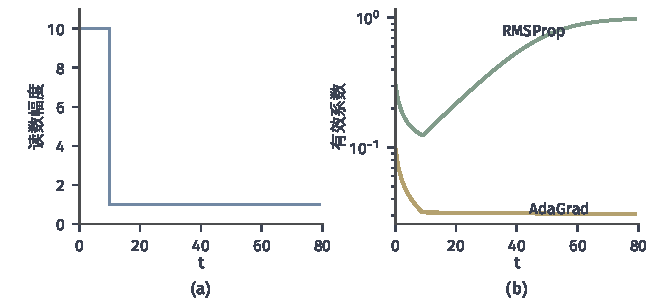
\includegraphics[width=112mm]{figures/05-optimization/05-stochastic-optimization/matplotlib/sgdb-adagrad-forget/figure.pdf}
  \caption{同一读数序列下的有效系数，$\alpha=1$，忽略稳定项。(a)读数幅度：前$10$轮为$10$，之后为$1$。(b)有效系数的对数图。黄线是AdaGrad，累计统计使系数一直偏小；绿线是$\rho=0.9$的RMSProp，大读数被遗忘后系数恢复到接近$1$。}
  \label{fig:sgdb-adagrad-forget}
\end{BookInlineFigure}

\paragraph{保证的范围}
AdaGrad的额外状态是一个$n$维向量，每轮额外计算量$O(n)$。保证按问题类型分别成立，引用时要注明。

\begin{itemize}
 \item 凸在线问题：对手依次给出凸损失，算法在有界可行域上行动，读数有界。评价对象是遗憾，也就是累计损失减去最好的固定决策的累计损失。原始分析给出$O(\sqrt T)$的遗憾，并在读数稀疏时有更好的常数\scite{duchi2011adagrad}。
 \item 随机凸问题：读数条件无偏时，可以由在线遗憾得到平均迭代的期望目标差，量级是$O(1/\sqrt T)$，同样需要有界可行域或相应的有界假设。
 \item 非凸光滑问题：评价对象是平方梯度范数的平均，需要读数有界或其他尾部条件，分母里的当前读数一般要特别处理。这类结果依赖具体的算法形式和假设，不能从凸的情形类推。
\end{itemize}

从更新形式本身推不出“比梯度下降快”。逐坐标缩放只有在问题的难点与坐标轴对齐时才有优势，图~\ref{fig:sgdb-adaptive-rotation}会展示这一边界。

\subsection{RMSProp}
\label{sec:sgdb-rmsprop}

\paragraph{用指数移动平均遗忘旧尺度}
AdaGrad难以遗忘，RMSProp把累计和换成\term{指数移动平均}（exponential moving average）\scite{hinton2012rmsprop}。取衰减系数$\rho\in[0,1)$，$\bm{s}^{(0)}=\bm{0}$：
\begin{equation}
 \bm{s}^{(t+1)}=\rho\bm{s}^{(t)}+(1-\rho)\hat{\bm g}^{(t)}\odot\hat{\bm g}^{(t)},\qquad
 \bm{x}^{(t+1)}=\bm{x}^{(t)}-\alpha\frac{\hat{\bm g}^{(t)}}{\sqrt{\bm{s}^{(t+1)}}+\epsilon}.
 \label{eq:sgdb-rmsprop}
\end{equation}

顺序与AdaGrad相同：先读，再用本轮读数更新$\bm{s}$，最后用新统计缩放本轮读数。$\epsilon$放在根号外，有的实现把它放在根号内，两者在分母很小时行为不同，记录实现时要写明。

展开递推，得到
\[
 \bm{s}^{(t+1)}=(1-\rho)\sum_{r=0}^{t}\rho^{t-r}\hat{\bm g}^{(r)}\odot\hat{\bm g}^{(r)}.
\]

$s$轮之前的读数平方的权重是$(1-\rho)\rho^{s}$，大约只记住最近$1/(1-\rho)$轮。$\rho=0.9$时约为$10$轮。

\paragraph{零初始化的早期偏差}
权重之和是$1-\rho^{t+1}$，早期小于$1$。读数恒为$g$时，
\[
 s^{(t+1)}=\bigl(1-\rho^{t+1}\bigr)g^2 ,
\]
早期分母偏小，有效系数偏大。表~\ref{tab:sgdb-adagrad-steps}的RMSProp列中，第一轮的系数是$1/\sqrt{0.1}\approx3.162$，比AdaGrad大得多。

再看图~\ref{fig:sgdb-adagrad-forget}的序列：前$10$轮把分母抬到约$8$，读数变小后，统计量大约以因子$\rho$逐轮衰减。第$30$轮的有效系数已经回到约$0.35$，第$79$轮约为$0.98$。

指数平均让尺度跟上最近的幅度，但它不提供一般的收敛保证。分母可能在大读数过后迅速变小，有效系数随之变大，下一节将看到这在特定问题上可能破坏收敛。

\subsection{Adam}
\label{sec:sgdb-adam}

\paragraph{主要思想}
RMSProp的分子只用当前读数。Adam在分子上也用移动平均，并修正两个平均的零初始化偏差\scite{kingma2015adam}。取$\beta_1,\beta_2\in[0,1)$，一阶统计$\bm{m}$与平方统计$\bm{s}$从零开始，读取本轮读数后依次计算
\begin{equation}
 \begin{aligned}
 \bm{m}^{(t+1)}&=\beta_1\bm{m}^{(t)}+(1-\beta_1)\hat{\bm g}^{(t)},\\
 \bm{s}^{(t+1)}&=\beta_2\bm{s}^{(t)}+(1-\beta_2)\hat{\bm g}^{(t)}\odot\hat{\bm g}^{(t)}.
 \end{aligned}
 \label{eq:sgdb-adam-stats}
\end{equation}

零初始化带来的偏差如何修正？展开$\bm{m}^{(t+1)}$，权重是$(1-\beta_1)\beta_1^{t-r}$，加起来是$1-\beta_1^{t+1}$，不是$1$。把统计量除以权重之和，得到两个修正量：
\begin{equation}
 \hat{\bm m}^{(t+1)}=\frac{\bm{m}^{(t+1)}}{1-\beta_1^{t+1}},\qquad
 \hat{\bm s}^{(t+1)}=\frac{\bm{s}^{(t+1)}}{1-\beta_2^{t+1}}.
 \label{eq:sgdb-adam-correction}
\end{equation}
读数恒为常数$\bm{g}$时，修正后$\hat{\bm m}^{(t+1)}=\bm{g}$，$\hat{\bm s}^{(t+1)}=\bm{g}\odot\bm{g}$，每一轮都恰好是常数读数的值。

参数更新使用修正后的量：
\begin{equation}
 \bm{x}^{(t+1)}=\bm{x}^{(t)}-\alpha\frac{\hat{\bm m}^{(t+1)}}{\sqrt{\hat{\bm s}^{(t+1)}}+\epsilon}.
 \label{eq:sgdb-adam-update}
\end{equation}

\begin{BookInlineFigure}
  \centering
  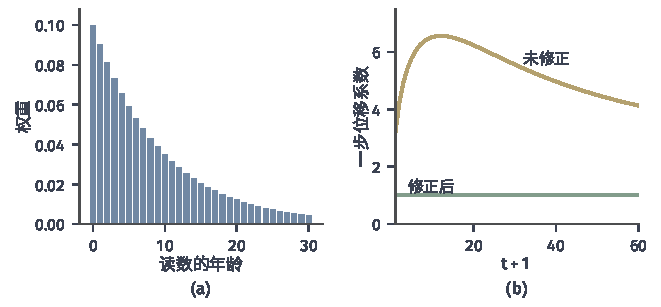
\includegraphics[width=112mm]{figures/05-optimization/05-stochastic-optimization/matplotlib/sgdb-adam-correction/figure.pdf}
  \caption{Adam的零初始化修正，$\beta_1=0.9$，$\beta_2=0.999$，读数恒为$1$，忽略稳定项。(a)$\bm{m}$的权重$(1-\beta_1)\beta_1^{s}$，$s$是读数的年龄。(b)一步位移的系数：黄线是未修正的$m/\sqrt{s}$，第一步约$3.16$，之后更大；绿线是修正后的$\hat m/\sqrt{\hat s}$，恒为$1$。}
  \label{fig:sgdb-adam-correction}
\end{BookInlineFigure}

图~\ref{fig:sgdb-adam-correction}(b)说明了修正的必要。$\beta_2$很接近$1$时，$\bm{s}$起步慢，未修正的$m/\sqrt{s}$在前几十轮都明显偏大，第$10$轮约为$6.5$。修正后系数恒为$1$。

\needspace{6\baselineskip}
\paragraph{变量}
\begin{itemize}
 \item $\bm{x}^{(t)}\in\mathbb{R}^n$：参数。
 \item $\bm{m}^{(t)},\bm{s}^{(t)}\in\mathbb{R}^n$：读数的一阶统计与平方统计。
 \item $t$：计时器，决定修正因子。
 \item $\alpha>0$，$\beta_1,\beta_2\in[0,1)$，$\epsilon>0$：步长、两个衰减系数、稳定项。
\end{itemize}

\paragraph{初始化}
令$\bm{m}^{(0)}=\bm{s}^{(0)}=\bm{0}$，$t=0$。例中是贯穿例的三项目标，取$\alpha=0.1$，$\beta_1=0.9$，$\beta_2=0.999$，读取顺序为第$3,1,2$项，手算时忽略$\epsilon$，起点和统计是
\[
 x^{(0)}=2,\qquad m^{(0)}=0,\qquad s^{(0)}=0.
\]

\needspace{6\baselineskip}
\paragraph{每轮更新}
在第$t$轮依次执行：
\begin{enumerate}
 \item \textbf{读取。}在当前点读取$\hat{\bm g}^{(t)}$。例中第一轮
 \[
  \hat g^{(0)}=f_3'(2)=-3.
 \]
 \item \textbf{更新统计。}按式~\eqref{eq:sgdb-adam-stats}计算$\bm{m}^{(t+1)}$和$\bm{s}^{(t+1)}$。例中第一轮
 \[
  m^{(1)}=0.1\cdot(-3)=-0.3,\qquad s^{(1)}=0.001\cdot9=0.009.
 \]
 \item \textbf{修正。}按式~\eqref{eq:sgdb-adam-correction}计算修正量。例中第一轮
 \[
  \hat m^{(1)}=\frac{-0.3}{0.1}=-3,\qquad \hat s^{(1)}=\frac{0.009}{0.001}=9.
 \]
 \item \textbf{更新参数。}按式~\eqref{eq:sgdb-adam-update}更新，然后$t\leftarrow t+1$。例中第一轮
 \[
  x^{(1)}=2-0.1\cdot\frac{-3}{3}=2.1.
 \]

 第二轮抽到第$1$项，读数和统计是
 \[
  \hat g^{(1)}=5.1,\qquad m^{(2)}=0.24,\qquad s^{(2)}=0.035001.
 \]
 两个修正分母是$1-0.81=0.19$和$1-0.998001=0.001999$，于是
 \[
  \hat m^{(2)}\approx1.2632,\qquad \hat s^{(2)}\approx17.509,\qquad \sqrt{\hat s^{(2)}}\approx4.184,
 \]
 参数更新为
 \[
  x^{(2)}=2.1-0.1\cdot\frac{1.2632}{4.184}\approx2.0698.
 \]

 第三轮抽到第$2$项，读数和统计是
 \[
  \hat g^{(2)}\approx4.1396,\qquad m^{(3)}\approx0.6300,\qquad s^{(3)}\approx0.052102.
 \]
 修正后
 \[
  \hat m^{(3)}\approx2.3246,\qquad \hat s^{(3)}\approx17.385,\qquad \sqrt{\hat s^{(3)}}\approx4.170,
 \]
 参数更新为
 \[
  x^{(3)}\approx2.0698-0.0558=2.0141.
 \]
\end{enumerate}

按预定轮数结束，例中$T=3$，最终得到$x^{(3)}\approx2.0141$。

\paragraph{修正偏差与优化方向的偏差}
修正因子只消除零初始化造成的权重不足，它不说明优化方向没有偏差。在上面的例子中，第二轮开始前$x^{(1)}=2.1$，$f'(2.1)=2.2$。固定历史后，$m^{(2)}$的条件均值是$0.9\cdot(-0.3)+0.1\cdot2.2=-0.05$，修正后的分子的条件均值约为
\[
 \frac{-0.05}{0.19}\approx-0.263 .
\]
它的符号甚至与$f'(2.1)$相反，原因是分子包含了上一轮的反向读数。分母还依赖本轮读数，所以式~\eqref{eq:sgdb-adam-update}的方向既不是当前梯度的无偏估计，也不是确定矩阵乘以当前梯度。

\paragraph{状态与保证}
Adam的状态包括$\bm{x}$、$\bm{m}$、$\bm{s}$和计时$t$。恢复运行时四项都要恢复：只恢复参数会丢失方向记忆；$t$错了，修正因子就错了。

Adam的原始论文给出了凸在线问题的分析，后来发现证明中存在问题，并有反例说明算法在一些凸问题上不收敛，下一小节说明这一点。引用Adam的保证时，必须对应具体的问题假设和参数设置，不能把一个具体分析中的结论当成算法的一般性质。

\paragraph{逐坐标缩放的边界}
图~\ref{fig:sgdb-adaptive-rotation}用精确梯度比较三种方法。目标是$f=(x_1^2+9x_2^2)/2$，起点$(9,1)$。主轴与坐标轴对齐时，AdaGrad第一步是$\alpha(1,1)$，随后逐坐标的尺度抵消了两个方向的曲率差异，到第$60$轮目标值约为$10^{-13}$。把目标和起点一起旋转$45^\circ$，陡峭方向不再对应一个坐标，AdaGrad到第$60$轮目标值约为$10^{-8}$，下降明显变慢。梯度下降对旋转不变，实线和虚线重合。

\begin{BookInlineFigure}
  \centering
  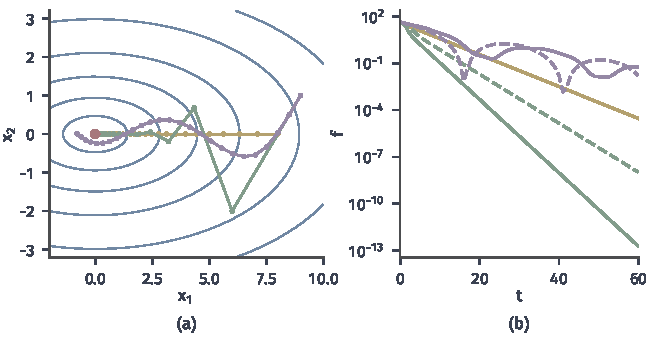
\includegraphics[width=112mm]{figures/05-optimization/05-stochastic-optimization/matplotlib/sgdb-adaptive-rotation/figure.pdf}
  \caption{逐坐标缩放与坐标系。目标$f=(x_1^2+9x_2^2)/2$，起点$(9,1)$，精确梯度。黄线是$\alpha=1/9$的梯度下降，绿线是$\alpha=3$的AdaGrad，紫线是$\alpha=0.5$的Adam（$\beta_1=0.9$，$\beta_2=0.999$）。(a)前$25$步的路径。(b)目标值：实线为原问题，虚线为把目标与起点一起旋转$45^\circ$后的同一问题，两条黄线重合。}
  \label{fig:sgdb-adaptive-rotation}
\end{BookInlineFigure}

\subsection{AMSGrad}
\label{sec:sgdb-amsgrad}

\paragraph{分母可能回落}
Adam和RMSProp的分母是指数平均，大读数过后可能迅速变小。分母一变小，有效步长就变大，此时的小读数被放大。这会造成什么后果？下面的构造说明，它足以让算法在一个凸问题上走向错误的方向\scite{reddi2018amsgrad}。

可行集是$[-1,1]$，读数依周期$3$变化，$C>2$：
\[
 \hat g^{(t)}=\begin{cases}C,& t\equiv1\pmod3,\\-1,&\text{其他}.\end{cases}
\]
对应的线性损失为$f_t(x)=\hat g^{(t)}x$，一个周期的总损失是$(C-2)x$，最优解是$x=-1$。取$C=3$，$\beta_1=0$（不用动量），$\beta_2=1/(1+C^2)=0.1$，步长$\alpha^{(t)}=0.1/\sqrt t$，更新后投影回$[-1,1]$。

\paragraph{一个周期内的净位移}
分母的三个值在稳态时循环。$s$按式~\eqref{eq:sgdb-adam-stats}递推，大读数$C$进入时升到约$8.207$，之后依次回落到$1.721$和$1.072$，所以一个周期的三个除数约为
\[
 \sqrt{8.207}\approx2.865,\qquad \sqrt{1.721}\approx1.312,\qquad \sqrt{1.072}\approx1.035.
\]
三步的位移与步长之比分别是$-3/2.865$，$+1/1.312$，$+1/1.035$，合计
\[
 -1.047+0.762+0.966=+0.681>0.
\]
一个周期的净位移是正的，迭代被推向错误的边界$x=+1$。大读数被大分母压低，小读数被回落的分母放大，方向信息就颠倒了。

\paragraph{算法}
AMSGrad让分母只增不减。分子和分母都不作零初始化修正，把历史最大的平方统计放进分母\scite{reddi2018amsgrad}。取$\bar{\bm s}^{(0)}=\bm{0}$，每轮在式~\eqref{eq:sgdb-adam-stats}之后计算
\begin{equation}
 \bar{\bm s}^{(t+1)}=\max\bigl\{\bar{\bm s}^{(t)},\bm{s}^{(t+1)}\bigr\},\qquad
 \bm{x}^{(t+1)}=\bm{x}^{(t)}-\alpha^{(t)}\frac{\bm{m}^{(t+1)}}{\sqrt{\bar{\bm s}^{(t+1)}}+\epsilon},
 \label{eq:sgdb-amsgrad}
\end{equation}
其中$\max$逐坐标取。

在上面的例子中，$\bar s$稳定在$8.207$，一个周期的位移与步长之比变为
\[
 \frac{-3+1+1}{2.865}\approx-0.349<0,
\]
净位移转为负，迭代走向$x=-1$。图~\ref{fig:sgdb-amsgrad-counter}的实际运行与此一致：Adam趋于$+1$，AMSGrad趋于$-1$。

\begin{BookInlineFigure}
  \centering
  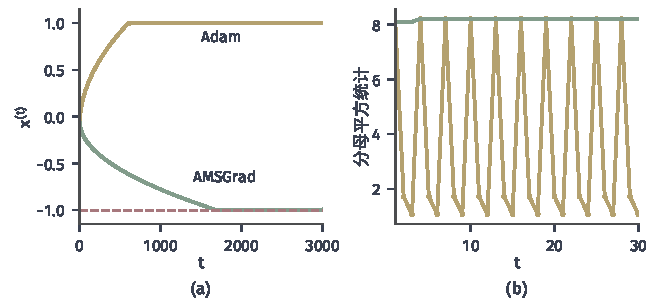
\includegraphics[width=112mm]{figures/05-optimization/05-stochastic-optimization/matplotlib/sgdb-amsgrad-counter/figure.pdf}
  \caption{周期线性目标上的Adam与AMSGrad，$C=3$，$\beta_1=0$，$\beta_2=0.1$，$\alpha^{(t)}=0.1/\sqrt t$，可行集$[-1,1]$。(a)迭代点，红色虚线是最优解$x=-1$。(b)分母中的平方统计：黄线是Adam随读数大幅涨落，绿线是AMSGrad保持最大值。}
  \label{fig:sgdb-amsgrad-counter}
\end{BookInlineFigure}

\paragraph{单调性是代数性质}
由更新规则，$\bar{\bm s}^{(t)}$逐坐标不减。若基步长$\alpha^{(t)}$不增，则每个坐标的有效缩放系数$\alpha^{(t)}/(\sqrt{\bar s_j^{(t)}}+\epsilon)$也不增。

这只是一个代数性质。它不说明目标值下降，也不说明算法收敛。AMSGrad的在线遗憾界需要凸性、有界可行域、有界读数，以及对$\beta_1^{(t)}$等参数的具体条件\scite{reddi2018amsgrad}；随机优化和非凸问题上的保证有各自的前提。不同问题上的结论不能互相代替。

\subsection{AdamW}
\label{sec:sgdb-adamw}

\paragraph{算法}
目标中常含平方惩罚$\frac\gamma2\lVert\bm{x}\rVert_2^2$。一种处理方式是把惩罚的梯度$\gamma\bm{x}$加到读数上，送进Adam的统计。另一种是\term{权重衰减}（weight decay）：历史统计只读取原目标的梯度，另外用更新前的参数单独收缩\scite{loshchilov2019adamw}。后一种方法称为AdamW，统计按式~\eqref{eq:sgdb-adam-stats}和式~\eqref{eq:sgdb-adam-correction}计算，参数更新改为
\begin{equation}
 \bm{x}^{(t+1)}=\bigl(1-\alpha^{(t)}\gamma\bigr)\bm{x}^{(t)}-\alpha^{(t)}\frac{\hat{\bm m}^{(t+1)}}{\sqrt{\hat{\bm s}^{(t+1)}}+\epsilon}.
 \label{eq:sgdb-adamw}
\end{equation}

收缩系数是$\alpha^{(t)}\gamma$，所以步长调度也带动收缩。对固定步长的随机梯度下降，两种做法相同：
\[
 \bm{x}-\alpha(\hat{\bm g}+\gamma\bm{x})=(1-\alpha\gamma)\bm{x}-\alpha\hat{\bm g}.
\]
但Adam的方向经过归一化，惩罚的梯度一旦进入统计，它的尺度也被归一化掉，两者不再相同。

\paragraph{同一标量首步比较}
取$x^{(0)}=1$，读数$\hat g^{(0)}=-0.1$，$\alpha=0.1$，$\gamma=0.5$，忽略$\epsilon$。第一轮的归一化方向等于读数的符号。AdamW用$\operatorname{sign}(-0.1)=-1$，按式~\eqref{eq:sgdb-adamw}，
\[
 x^{(1)}=(1-0.05)\cdot1+0.1=1.05.
\]

把惩罚梯度并入读数时，并入后的读数是$-0.1+0.5\cdot1=0.4$，符号变成$+1$，于是
\[
 x^{(1)}=1-0.1=0.9.
\]

两种做法的位移方向相反。图~\ref{fig:sgdb-adamw-step}显示了$\gamma$变化时的情况：AdamW的第一步关于$\gamma$连续变化；并入读数的做法在$\gamma=0.1$处突变，符号翻转后位移就不再随$\gamma$改变，惩罚的大小被归一化抹去了。

\begin{BookInlineFigure}
  \centering
  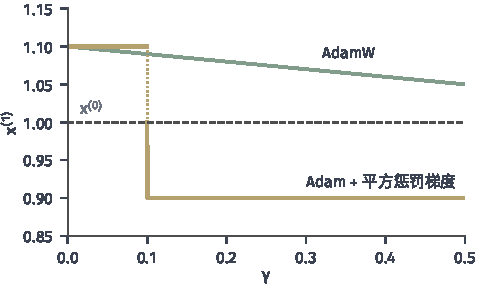
\includegraphics[width=82mm]{figures/05-optimization/05-stochastic-optimization/matplotlib/sgdb-adamw-step/figure.pdf}
  \caption{首步$x^{(1)}$关于惩罚系数$\gamma$的变化，$x^{(0)}=1$，$\hat g^{(0)}=-0.1$，$\alpha=0.1$。绿线是AdamW，黄线是把惩罚梯度并入读数后的Adam，虚线是起点。}
  \label{fig:sgdb-adamw-step}
\end{BookInlineFigure}

AdamW与平方惩罚并入读数的做法，优化的不是同一个迭代过程，它们停止的位置一般也不同。评价时要看实际定义的目标：返回点的目标值应写明是否包含惩罚项，收缩系数$\gamma$的含义也要随之说明。

\subsection{Adafactor统计压缩（补充）}
\label{sec:sgdb-adafactor}

\paragraph{用行列边际近似平方统计}
参数是矩阵$\bm{W}\in\mathbb{R}^{m\times d}$时，Adam的平方统计要存$md$个数。Adafactor只存平方统计的行和$\bm{r}\in\mathbb{R}^m$与列和$\bm{c}\in\mathbb{R}^d$，需要时重建近似的平方统计\scite{shazeer2018adafactor}。

设完整的平方统计是$\bm{V}$，$\bm{r}=\bm{V}\bm{1}_d$，$\bm{c}=\bm{V}^\top\bm{1}_m$。假定$\bm{V}$接近秩一，重建公式是
\begin{equation}
 \hat{\bm V}=\frac{\bm{r}\bm{c}^\top}{\bm{1}_m^\top\bm{r}} .
 \label{eq:sgdb-adafactor}
\end{equation}
分母是$\bm{V}$所有元素的和，这一归一化使重建保持行和与列和：$\hat{\bm V}\bm{1}_d=\bm{r}$，$\hat{\bm V}^\top\bm{1}_m=\bm{c}$。存储量从$md$降到$m+d$。

\paragraph{更新的次序}
一轮的次序是：先在读数的平方上加稳定项$\epsilon_1$，得到$\hat{\bm G}^{(t)}\odot\hat{\bm G}^{(t)}+\epsilon_1$，保证重建的分母为正；再分别用其行和与列和更新$\bm{r}$、$\bm{c}$的移动平均；然后由式~\eqref{eq:sgdb-adafactor}重建$\hat{\bm V}$；再求方向$\bm{Y}=\hat{\bm G}^{(t)}/\sqrt{\hat{\bm V}}$，把方向按均方根裁剪，最后乘以相对步长更新参数。相对步长与参数自身的均方根成正比，并有下界$\epsilon_2$。

这三件事分开算：统计压缩改变了尺度的来源，方向裁剪改变了方向的大小，相对步长改变了位移的量纲。评价改动带来的差别时，也要分别考虑。

\paragraph{保留与丢失的信息}
重建精确的条件很简单。若$\bm{V}$元素全为正，$\hat{\bm V}=\bm{V}$当且仅当$\bm{V}$秩为一，因为$\hat{\bm V}$按构造秩为一。例如
\[
 \bm{V}=\begin{bmatrix}1&2\\3&6\end{bmatrix}
\]
秩为一，行和是$(3,9)$，列和是$(4,8)$，总和是$12$，重建给出原矩阵。而
\[
 \bm{V}=\begin{bmatrix}4&1\\1&4\end{bmatrix}
\]
的行和、列和都是$(5,5)$，重建得到所有元素都是$2.5$的矩阵，对角线上的大值和非对角线的小值被抹平。

图~\ref{fig:sgdb-adafactor-recon}给出一个$6\times8$的例子。大尺度的行列结构被保留，逐元素的相对误差平均约为$0.13$，最大约为$0.70$。

\begin{BookInlineFigure}
  \centering
  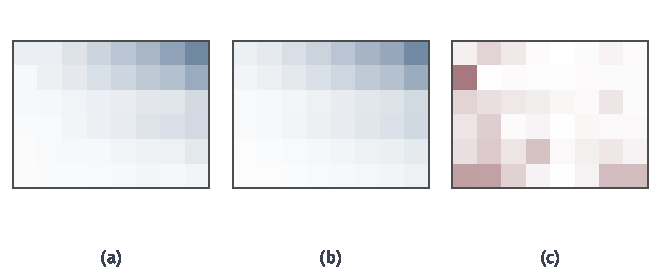
\includegraphics[width=112mm]{figures/05-optimization/05-stochastic-optimization/matplotlib/sgdb-adafactor-recon/figure.pdf}
  \caption{平方统计的行列压缩。(a)由$40$个随机读数算出的逐元素平方平均$\bm{V}$，形状$6\times8$。(b)按式~\eqref{eq:sgdb-adafactor}由$6$个行和与$8$个列和重建的$\hat{\bm V}$。(c)逐元素相对误差。颜色越深数值越大。}
  \label{fig:sgdb-adafactor-recon}
\end{BookInlineFigure}

压缩减少的只是统计的存储。参数、读数和方向仍是$md$个数；总计算量不会因此变成$O(m+d)$。低存储也不意味着收敛更快，近似的统计改变了方向，效果要回到目标上评价。

\subsection{Shampoo矩阵预条件（补充）}
\label{sec:sgdb-shampoo}

\paragraph{左右Gram统计}
逐坐标的尺度无法描述“某几行一起变化”这样的方向关系。Shampoo为矩阵参数维护左右两个Gram统计，分别刻画行空间和列空间方向的历史幅度\scite{gupta2018shampoo}。取$\epsilon>0$，$\bm{L}^{(0)}=\epsilon\bm{I}_m$，$\bm{R}^{(0)}=\epsilon\bm{I}_d$，读取矩阵读数$\hat{\bm G}^{(t)}$后先更新统计：
\begin{equation}
 \bm{L}^{(t+1)}=\bm{L}^{(t)}+\hat{\bm G}^{(t)}\hat{\bm G}^{(t)\top},\qquad
 \bm{R}^{(t+1)}=\bm{R}^{(t)}+\hat{\bm G}^{(t)\top}\hat{\bm G}^{(t)},
 \label{eq:sgdb-shampoo-stats}
\end{equation}
再用两侧的负四分之一次幂更新：
\begin{equation}
 \bm{W}^{(t+1)}=\bm{W}^{(t)}-\alpha\bigl(\bm{L}^{(t+1)}\bigr)^{-1/4}\hat{\bm G}^{(t)}\bigl(\bm{R}^{(t+1)}\bigr)^{-1/4}.
 \label{eq:sgdb-shampoo}
\end{equation}

$\epsilon$使两个统计正定，负四分之一次幂才有定义。按正交对角化计算：
\[
 \bm{L}=\bm{Q}\operatorname{diag}(\lambda_j)\bm{Q}^\top
 \quad\Longrightarrow\quad
 \bm{L}^{-1/4}=\bm{Q}\operatorname{diag}\bigl(\lambda_j^{-1/4}\bigr)\bm{Q}^\top .
\]
正交对角化可参考\BookChapterRef{chap:eigen-spectral-decomposition}{卷二第6章“谱分解”}。这两个矩阵是读数的累计，不是目标的Hessian。

\paragraph{单步：奇异值被拉平}
取$\epsilon\to0$，方阵可逆读数$\bm{G}=\bm{U}\bm{\Sigma}\bm{V}^\top$。则$\bm{G}\bm{G}^\top=\bm{U}\bm{\Sigma}^2\bm{U}^\top$，$\bm{G}^\top\bm{G}=\bm{V}\bm{\Sigma}^2\bm{V}^\top$，代入式~\eqref{eq:sgdb-shampoo}，
\[
 \bigl(\bm{G}\bm{G}^\top\bigr)^{-1/4}\bm{G}\bigl(\bm{G}^\top\bm{G}\bigr)^{-1/4}
 =\bm{U}\bm{\Sigma}^{-1/2}\bm{\Sigma}\bm{\Sigma}^{-1/2}\bm{V}^\top=\bm{U}\bm{V}^\top .
\]
一步的效果与Muon的理想极因子相同，所有奇异值都变成$1$。例如$\bm{G}=\operatorname{diag}(4,1/4)$时，两侧的变换都是$\operatorname{diag}(1/2,2)$，变换后得到$\bm{I}$，两个方向相差$16$倍的幅度被拉平。

累积多步之后不再这样简单。统计综合了历史上各方向的幅度，变换后的奇异值不等于$1$，并且随累积的读取逐渐减小，图~\ref{fig:sgdb-shampoo-flatten}(b)显示了这一点。这是累计式缩放的共同特点，与AdaGrad的有效系数逐渐减小相同。

\begin{BookInlineFigure}
  \centering
  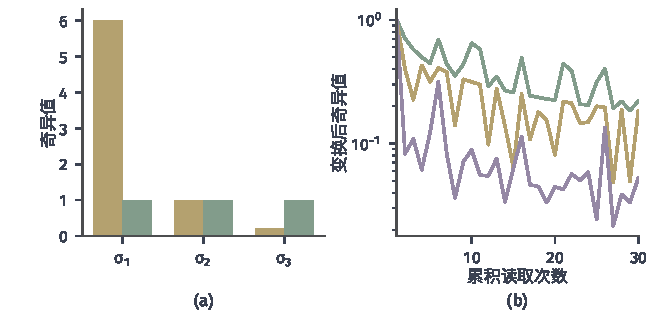
\includegraphics[width=112mm]{figures/05-optimization/05-stochastic-optimization/matplotlib/sgdb-shampoo-flatten/figure.pdf}
  \caption{Shampoo的奇异值变换，$\epsilon=10^{-6}$，$\bm{G}$是$3\times3$矩阵，奇异值为$6,1,0.2$。(a)单步：原始奇异值（黄）与式~\eqref{eq:sgdb-shampoo}变换后的奇异值（绿）。(b)累积读取时，变换后的三个奇异值随读取次数的变化，读数的各方向幅度随机变化。}
  \label{fig:sgdb-shampoo-flatten}
\end{BookInlineFigure}

\paragraph{计算成本}
Shampoo的额外成本比逐坐标方法高得多。统计的存储是$O(m^2+d^2)$；形成两个Gram矩阵需要$O(m^2d+md^2)$次运算；稠密谱分解求矩阵根一次约$O(m^3+d^3)$；两侧作用变换是$O(m^2d+md^2)$。

求根最贵，实际实现常隔若干步才重新计算根，中间继续使用旧因子。这样本轮使用的尺度来自若干步之前的统计，与式~\eqref{eq:sgdb-shampoo}“先更新后使用”不是同一个算法，记录时要写明刷新频率。比较方法时，统计存储、分解、旧因子的使用以及每步的乘法都要计入，不能只比较更新次数。

\section{梯度的处理}
\label{sec:sgdb-processing}

前两节的方向都由读数线性组合或缩放而来。本节研究更直接的改动：读数被截短、用有限精度算出、来自过去的点，甚至换成一个人为规定的向量。这些操作都使实际方向偏离原目标的梯度。

实际方向在什么点上、以什么误差近似当前梯度，这个误差怎样影响原目标上的进展？回答时把实际读数分解成三部分：真梯度$\bm{g}^{(t)}$、由历史确定的条件偏差$\bm{b}^{(t)}$、零条件均值的噪声$\bm{\xi}^{(t)}$，
\begin{equation}
 \hat{\bm g}^{(t)}=\bm{g}^{(t)}+\bm{b}^{(t)}+\bm{\xi}^{(t)},\qquad
 \mathbb{E}\bigl[\bm{\xi}^{(t)}\mid\mathcal{F}^{(t)}\bigr]=\bm{0}.
 \label{eq:sgdb-reading-decomposition}
\end{equation}

这个分解在前面的读数误差分析中已经用过，这里偏差项不再为零。下面分别看裁剪、近似和替代三种情形下$\bm{b}^{(t)}$从哪里来、能否被控制。

\subsection{梯度裁剪}
\label{sec:sgdb-clipping}

\paragraph{两种裁剪}
\term{梯度裁剪}（gradient clipping）在读数过大时把它截短，防止个别很大的读数把参数推得太远\scite{pascanu2013}。给定阈值$c>0$，有两种做法。\term{逐坐标裁剪}（coordinate-wise clipping）把每个坐标截到$[-c,c]$内：
\begin{equation}
 \bigl[\operatorname{clip}^{\mathrm{co}}_c(\bm{g})\bigr]_j=\max\{-c,\min\{c,g_j\}\}.
 \label{eq:sgdb-clip-coord}
\end{equation}

\term{范数裁剪}（norm clipping）整体缩放，只在范数超过阈值时起作用：
\begin{equation}
 \operatorname{clip}_c(\bm{g})=\bm{g}\cdot\min\Bigl\{1,\frac{c}{\lVert\bm{g}\rVert_2}\Bigr\}.
 \label{eq:sgdb-clip-norm}
\end{equation}

下面用同一个读数比较。取$\bm{g}=(3,4)$，$c=1$，两种裁剪的结果是
\[
 \operatorname{clip}^{\mathrm{co}}_1(\bm{g})=(1,1),\qquad
 \operatorname{clip}_1(\bm{g})=(0.6,0.8).
\]

前者的范数是$\sqrt2$，方向从与第一坐标轴夹角约$53^\circ$变成$45^\circ$；后者的范数是$1$，方向不变。图~\ref{fig:sgdb-clip-bias}(a)表明，逐坐标裁剪是投影到边长$2c$的正方形，范数裁剪是投影到半径$c$的圆盘。

\begin{BookInlineFigure}
  \centering
  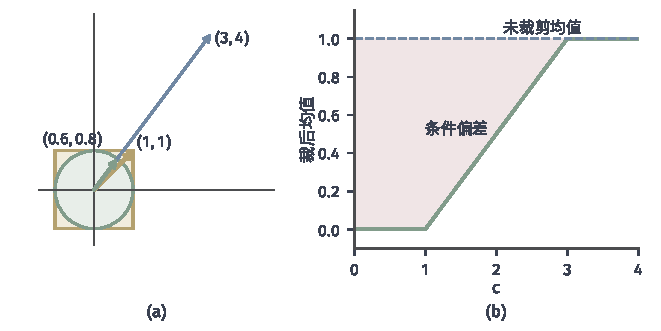
\includegraphics[width=112mm]{figures/05-optimization/05-stochastic-optimization/matplotlib/sgdb-clip-bias/figure.pdf}
  \caption{裁剪的几何与偏差。(a)读数$(3,4)$（蓝）在$c=1$时的两种裁剪：逐坐标裁剪得到黄色正方形角上的$(1,1)$；范数裁剪沿原方向缩到绿色圆上的$(0.6,0.8)$。(b)读数以相等概率取$3$或$-1$，绿线是逐点裁剪后的均值关于阈值$c$的变化，蓝色虚线是未裁剪的均值$1$，红色区域是两者之差。}
  \label{fig:sgdb-clip-bias}
\end{BookInlineFigure}

\paragraph{裁剪放在哪里}
一个算法中可以裁剪的位置不止一处，图~\ref{fig:sgdb-clip-position}标出了四处。裁剪位置$1$：裁剪逐样本读数后再平均，后面的动量和统计看到的都是裁过的量。裁剪位置$2$：先平均再裁剪批量读数。裁剪位置$3$：裁剪动量方向，统计仍记录原始读数。裁剪位置$4$：裁剪缩放后的方向，也就是最终的位移。

\begin{BookInlineFigure}
  \centering
  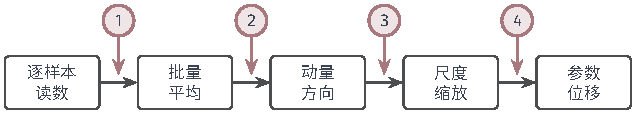
\includegraphics[width=107.64mm]{figures/05-optimization/05-stochastic-optimization/tikz/sgdb-clip-position/figure.pdf}
  \caption{更新流水线上可以施加裁剪的四个位置，圆圈内的数字对应正文的编号。位置不同，得到的是不同的算法，描述一次运行时要写明位置和阈值。}
  \label{fig:sgdb-clip-position}
\end{BookInlineFigure}

位置$1$和位置$2$的差别，用贯穿例在$x=2$处的三项读数说明。取$c=2$，全批量读数$5,4,-3$。先逐项裁剪再平均，得到
\[
 \frac13\bigl(2+2-2\bigr)=\frac23.
\]
先平均再裁剪，平均是$f'(2)=2$，未超过阈值，裁剪不起作用，得到$2$。前者有偏差，后者这里没有。

增大批量能否减小偏差，也取决于位置。逐样本裁剪后再平均，批量越大，平均越接近裁后读数的均值，偏差不随批量变小。先平均再裁剪时，批量越大，平均读数越集中在真梯度附近，只要真梯度的范数小于阈值，被裁剪的概率就越小，偏差随之减小。

\paragraph{用两点分布核对偏差}
裁剪是非线性运算，它改变读数的平均。设读数以相等概率取$3$与$-1$，均值为$1$。用$c=1$裁剪后，读数变为$1$与$-1$，均值为$0$：
\[
 \mathbb{E}\bigl[\operatorname{clip}_1(\hat g)\bigr]=0\neq1.
\]

条件偏差是$-1$，等于真梯度的相反数，方向信息完全消失。图~\ref{fig:sgdb-clip-bias}(b)画出裁后均值随阈值的变化：$c<1$时为$0$，$1\leq c<3$时为$(c-1)/2$，$c\geq3$时才恢复为$1$。

所以裁后的读数不能当作无偏梯度套用前面的定理。贯穿例能说明后果。取$c=2$的逐项裁剪，期望方向在$x=0$处为
\[
 \frac13\bigl(\operatorname{clip}_2(3)+\operatorname{clip}_2(0)+\operatorname{clip}_2(-9)\bigr)=\frac13(2+0-2)=0.
\]
也就是说，逐项裁剪的均值在$x=0$处恰好为零，而真正的最优点是$x^\star=1$，$f(0)-f^\star=1$。裁剪把期望更新的平衡点从$x=1$移到了$x=0$。

\paragraph{分别评价两种作用}
裁剪的作用要分开评价。第一是控制位移：范数裁剪在位置$2$或位置$4$保证每步位移的范数不超过$\alpha c$，这是确定的。第二是控制二阶矩：裁后读数的范数不超过$c$，所以它的二阶矩不超过$c^2$。原读数的二阶矩很大甚至无穷时，裁剪之后前面依赖方差假设的分析才可能使用。

这两种好处的代价是偏差$\bm{b}^{(t)}$。偏差怎样影响进展，由下一小节的递推回答。是否值得用偏差换取有界的二阶矩，要看具体的读数分布，没有无条件的结论。

\subsection{近似梯度}
\label{sec:sgdb-approximate}

\paragraph{几种来源}
实际得到的方向常常不是当前点的精确读数。下面三种情形都先问两件事：方向在哪个求值点上计算，误差能否由计算预算或步长控制。

第一是有限精度。例如浮点运算或内层线性方程只解到某个残差，读到的是$\nabla f(\bm{x}^{(t)})$的近似，误差$\bm{b}^{(t)}$的大小由内层的求解精度决定，增加每步计算可以使它变小。第二是量化，把读数的每个分量化到间距$\Delta$的格点上，$\lvert b_j\rvert\leq\Delta/2$，这是确定的偏差。真梯度比半个格子还小时，量化后的读数恰好是零，迭代会停在一个有残差的点上。第三是延迟读取，在第$t$轮用$\tau$轮之前的点上的梯度$\nabla f(\bm{x}^{(t-\tau)})$，也就是求值点不是当前点。

延迟的误差由步长控制，但可能破坏稳定性。设$f(x)=\frac12x^2$，用延迟$\tau=1$的精确梯度，
\[
 x^{(t+1)}=x^{(t)}-\alpha x^{(t-1)}.
\]
特征方程是$r^2-r+\alpha=0$。当$\alpha\in(0,1)$时，两根的模都小于$1$：两根为实数时积为$\alpha$，和为$1$，都在$(0,1)$内；两根共轭时模的平方等于积$\alpha$。当$\alpha=1$时两根落在单位圆上，迭代恰好以周期$6$循环。没有延迟时，$\alpha$可以取到$2$，所以延迟把稳定的步长范围缩小了一半。图~\ref{fig:sgdb-bias-delay}(b)是$\alpha=1$的情形，$\tau=2$时发散。

\begin{BookInlineFigure}
  \centering
  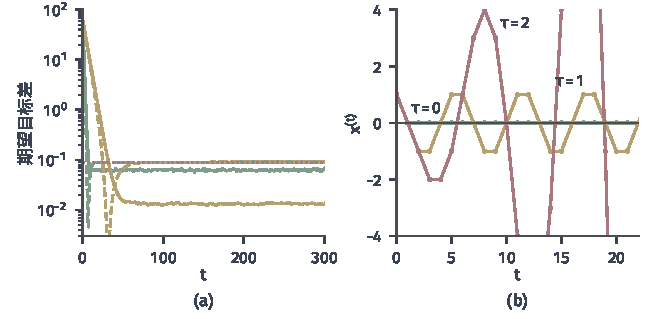
\includegraphics[width=112mm]{figures/05-optimization/05-stochastic-optimization/matplotlib/sgdb-bias-delay/figure.pdf}
  \caption{偏差、噪声与延迟的影响。(a)目标$f(x)=(x-1)^2+5$，初值$x=9$，$2000$次独立运行的平均目标差，绿线$\alpha=0.2$，黄线$\alpha=0.05$。实线是只有方差为$1$的噪声；虚线是只有常数偏差$b=0.6$，两种步长最终都停在红色点线$b^2/4=0.09$上。(b)目标$\frac12x^2$，$\alpha=1$，延迟$\tau=0,1,2$的迭代点。}
  \label{fig:sgdb-bias-delay}
\end{BookInlineFigure}

\paragraph{把偏差和噪声代入递推}
现在按式~\eqref{eq:sgdb-reading-decomposition}把两类误差代入有限步递推。下面的结果与前面的无偏分析结构相同，只多了偏差产生的一项。

\begin{theorem}[有偏读数下的平均平方梯度范数]
\label{thm:sgdb-biased}
设$f$梯度$L$-Lipschitz连续，下确界为$f_{\inf}$。设读数满足式~\eqref{eq:sgdb-reading-decomposition}，其中$\bm{b}^{(t)}$由$\mathcal{F}^{(t)}$确定，并且
\begin{equation}
 \lVert\bm{b}^{(t)}\rVert_2\leq B,\qquad
 \mathbb{E}\bigl[\lVert\bm{\xi}^{(t)}\rVert_2^2\mid\mathcal{F}^{(t)}\bigr]\leq\sigma^2 .
 \label{eq:sgdb-biased-condition}
\end{equation}
取固定步长$0<\alpha\leq1/L$，用$\hat{\bm g}^{(t)}$代替梯度做一步更新。则
\begin{equation}
 \mathbb{E}\bigl[f(\bm{x}^{(t+1)})\mid\mathcal{F}^{(t)}\bigr]\leq f(\bm{x}^{(t)})-\frac\alpha2\lVert\bm{g}^{(t)}\rVert_2^2+\frac\alpha2B^2+\frac{L\alpha^2}{2}\sigma^2,
 \label{eq:sgdb-biased-step}
\end{equation}
因而
\begin{equation}
 \frac1T\sum_{t=0}^{T-1}\mathbb{E}\lVert\bm{g}^{(t)}\rVert_2^2\leq\frac{2\bigl(f(\bm{x}^{(0)})-f_{\inf}\bigr)}{\alpha T}+B^2+L\alpha\sigma^2 .
 \label{eq:sgdb-biased-bound}
\end{equation}
\end{theorem}

\begin{proof}
由下降引理，
\[
 f(\bm{x}^{(t+1)})\leq f(\bm{x}^{(t)})-\alpha\langle\bm{g}^{(t)},\hat{\bm g}^{(t)}\rangle+\frac{L\alpha^2}{2}\lVert\hat{\bm g}^{(t)}\rVert_2^2 .
\]

记$\bm{a}=\bm{g}^{(t)}+\bm{b}^{(t)}$，它由历史确定。固定$\mathcal{F}^{(t)}$取条件期望。噪声的条件均值为零，所以交叉项消失，
\[
 \mathbb{E}\langle\bm{g}^{(t)},\hat{\bm g}^{(t)}\rangle=\langle\bm{g}^{(t)},\bm{a}\rangle,\qquad
 \mathbb{E}\lVert\hat{\bm g}^{(t)}\rVert_2^2\leq\lVert\bm{a}\rVert_2^2+\sigma^2 .
\]

由$\alpha\leq1/L$，$L\alpha^2/2\leq\alpha/2$，于是$\lVert\bm{a}\rVert_2^2$前的系数可以放大到$\alpha/2$，得到
\[
 \mathbb{E}f(\bm{x}^{(t+1)})\leq f(\bm{x}^{(t)})-\alpha\langle\bm{g}^{(t)},\bm{a}\rangle+\frac\alpha2\lVert\bm{a}\rVert_2^2+\frac{L\alpha^2}{2}\sigma^2 .
\]

展开平方并配方，
\[
 -\alpha\langle\bm{g}^{(t)},\bm{a}\rangle+\frac\alpha2\lVert\bm{a}\rVert_2^2
 =\frac\alpha2\bigl(\lVert\bm{a}-\bm{g}^{(t)}\rVert_2^2-\lVert\bm{g}^{(t)}\rVert_2^2\bigr)
 =\frac\alpha2\bigl(\lVert\bm{b}^{(t)}\rVert_2^2-\lVert\bm{g}^{(t)}\rVert_2^2\bigr).
\]

代入$\lVert\bm{b}^{(t)}\rVert_2\leq B$，得到式~\eqref{eq:sgdb-biased-step}。对$t=0,\ldots,T-1$取全期望并累加，用$f(\bm{x}^{(T)})\geq f_{\inf}$，两边除以$\alpha T/2$，得到式~\eqref{eq:sgdb-biased-bound}。
\end{proof}

式~\eqref{eq:sgdb-biased-bound}有三项。第一项是初始误差，随$T$消失。第三项是噪声，正比于$\alpha$，可以用小步长或小批量压低。第二项$B^2$既不依赖$\alpha$，也不依赖$T$。

图~\ref{fig:sgdb-bias-delay}(a)验证了这一分工。只有噪声时，$\alpha$从$0.2$减到$0.05$，平台约从$0.0625$降到$0.0132$，与$\alpha/(2(2-2\alpha))$一致。只有常数偏差时，两种步长最终停在同一高度$b^2/4=0.09$，小步长只是到达得更慢。

\paragraph{上界中的残余不是下限}
$B^2$是上界中的项，不是误差的下限。偏差项能否真的造成残余，取决于偏差的结构。

设$f(x)=\frac12x^2$，常数偏差$b$使读数的均值变成$x+b$，迭代的平衡点是$x=-b$，平方梯度是$b^2$，这时界是紧的。如果偏差随梯度变小，满足
\[
 \lVert\bm{b}^{(t)}\rVert_2\leq\rho\lVert\bm{g}^{(t)}\rVert_2,\qquad\rho<1,
\]
回到证明中的配方等式，确定部分的下降量至少是$\frac\alpha2(1-\rho^2)\lVert\bm{g}^{(t)}\rVert_2^2$，平方梯度可以趋于零。裁剪在读数范数以概率$1$小于阈值时偏差恰好为零，这时实际残余也小于用$B^2$估计的量。

\subsection{替代梯度（补充）}
\label{sec:sgdb-surrogate}

\paragraph{导数没有用处的前向函数}
前向函数有时是分段常数，经典梯度几乎处处为零。设$Q(w)=\lfloor w+\tfrac12\rfloor$是取整，损失为
\begin{equation}
 F(w)=\frac12\bigl(Q(w)-a\bigr)^2 .
 \label{eq:sgdb-rounding}
\end{equation}

$Q$在非半整数点局部为常数，所以除了可数个跳跃点外$F'(w)=0$，导数不提供任何信息。梯度下降一步也不会动。

\paragraph{人为指定的反向规则}
\term{直通估计}（straight-through estimator）在反向计算时假装$Q$是恒等映射，规定$\mathrm{d}Q/\mathrm{d}w=1$\scite{math-bengio2013estimating}，返回的方向是
\begin{equation}
 g_{\mathrm{STE}}(w)=Q(w)-a .
 \label{eq:sgdb-ste}
\end{equation}

这类人为指定的方向统称\term{替代梯度}（surrogate gradient）。要区分两件事：前向函数$F$是实际被评价的对象，反向规则是另外选的方向生成方式，两者之间没有求导关系。在计算图中还常用\term{停止梯度}（stop-gradient）这一传播规则写成$w+\operatorname{sg}(Q(w)-w)$，其中$\operatorname{sg}$前向原样传值，反向阻断传播；前向得到$Q(w)$，反向等于恒等映射。它是计算图上的规则，不是数学运算的导数。

\paragraph{跨阈值的两次更新}
图~\ref{fig:sgdb-ste-round}给出同一点出发的两个结果。取$w=0.3$，此时$Q(w)=0$。若$a=1$，损失是$F=0.5$，替代方向是$-1$，取步长$0.4$走到$w=0.7$，此时$Q=1$，损失降到
\[
 F(0.7)=\frac12(1-1)^2=0.
\]

若$a=0.3$，损失是$F=0.045$，替代方向是$-0.3$，取步长$4/3$同样走到$w=0.7$，损失却升到
\[
 F(0.7)=\frac12(1-0.3)^2=0.245.
\]

光滑情形下的下降依赖于“小步之内一阶模型准确”，而跨过跳跃点时一阶模型完全失效。所以无法从替代方向推出下降。

\begin{BookInlineFigure}
  \centering
  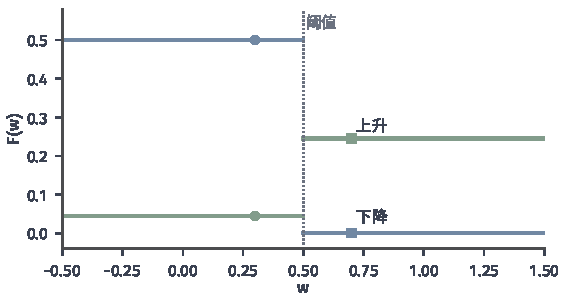
\includegraphics[width=96mm]{figures/05-optimization/05-stochastic-optimization/matplotlib/sgdb-ste-round/figure.pdf}
  \caption{取整前向上的直通更新。蓝线$F(w)=\frac12(Q(w)-1)^2$，绿线$F(w)=\frac12(Q(w)-0.3)^2$，都是分段常数，点线是取整阈值$w=0.5$。圆点是起点$w=0.3$，方块是走一步后的$w=0.7$：蓝色的损失由$0.5$降到$0$，绿色的损失由$0.045$升到$0.245$。}
  \label{fig:sgdb-ste-round}
\end{BookInlineFigure}

\paragraph{替代方向的地位}
替代方向既不是原目标的经典梯度，一般也不是凸次梯度。以$a=1$，$w=0.3$为例，若$s$是全局次梯度，要求不等式$F(y)\geq F(0.3)+s(y-0.3)$对一切$y$成立。

取$y=0.7$，得到$0\geq0.5+0.4s$，即$s\leq-1.25$。取$y=-0.4$，$F(-0.4)=0.5$，得到$s\geq0$。两者矛盾，这样的$s$不存在，$F$在该点没有全局次梯度，$-1$更不是。局部上$F$在该点附近为常数，局部的次梯度只有$0$，也不是$-1$。

所以使用替代方向的算法，只能回到实际的前向目标上评价。比较的量应是前向损失或原问题的目标值，停止准则也应基于前向量，而不是替代方向的范数是否变小。

\section{误差与计算成本}
\label{sec:sgdb-cost}

本章已经出现了很多方法，每一种都有自己的误差界和成本描述。它们能不能放在一起比较？回答这个问题，先要固定三件事：要最小化哪个目标，算法返回什么，用什么量计算成本。本节依次讨论评价对象、总计算成本，以及当输入的数据发生变化时算法的有限步响应。

\subsection{误差的评价对象}
\label{sec:sgdb-error-objects}

\paragraph{量与返回点的配对}
一个收敛结论由两部分组成：度量什么量，度量哪个点。常用的量有目标差、到最小点的距离、梯度范数或邻近残差；常用的返回点有最后一点、平均点和随机返回点。量和点的配对不能互换，表~\ref{tab:sgdb-error-pairing}列出常见的配对。

\begin{BookInlineTable}
  \centering
  \caption{常见的误差量与返回点的配对。条件只列出主要假设，具体常数和步长以相应结论为准。}
  \label{tab:sgdb-error-pairing}
  \begin{tabular}{lll}
    \toprule
    误差量 & 返回点 & 主要条件\\
    \midrule
    期望目标差 & 加权平均点 & 凸\\
    期望目标差 & 最后一点 & 强凸\\
    到最小点的距离 & 最后一点 & 强凸\\
    平方梯度范数 & 按权重随机返回 & 光滑非凸\\
    邻近残差 & 按权重随机返回 & 复合目标\\
    \bottomrule
  \end{tabular}
\end{BookInlineTable}

配对的差别可以在贯穿例上看见。常步长$\alpha=0.1$时，随机梯度下降的最后一点的期望目标差趋于$0.528$，不随轮数继续下降。模拟$20$万条路径，后$2000$轮的平均点的期望目标差约为$0.0024$，比最后一点小两个多量级。平均减小了噪声，但关于平均点的界不能直接移用到某个单独的迭代点上。

\paragraph{期望保证与概率保证}
上面的误差界都是期望。期望小不等于每次运行都小。若$Z\geq0$是目标差，$\mathbb{E}Z\leq\varepsilon$，由Markov不等式，对任意$\delta\in(0,1)$，
\begin{equation}
 \mathbb{P}\Bigl(Z\geq\frac{\varepsilon}{\delta}\Bigr)\leq\delta .
 \label{eq:sgdb-markov}
\end{equation}

比如$\mathbb{E}Z\leq0.01$，只能得到目标差超过$0.1$的概率不超过$0.1$。这里$\varepsilon/\delta$随$\delta$变小放大得很快。更强的高概率保证需要读数的尾部条件，例如有界或次高斯，并使用鞅集中不等式，推导要用到鞅的工具，这里只说明它与期望保证的区别。

路径的长期性质是另一个问题，例如一条路径是否几乎必然收敛，这类结论依赖步长条件和鞅收敛定理，属于前面提到的长期路径分析。有限步的期望界不能回答这个问题。

\paragraph{各类误差进入递推的位置}
本章遇到的误差进入递推的不同位置。条件噪声进入二次项，贡献$\sigma^2$乘以步长的相应幂次，能靠减小步长或增大批量压低。系统偏差进入一次项，贡献的$B^2$不随步长变小。近似求解的误差与偏差类似，由内层精度决定。

这些都是\term{优化误差}（optimization error），针对的是给定的目标。如果目标是由一批样本构造的有限和，而真正关心的是总体上的目标，那么还有一部分由样本有限造成的差距。这部分属于统计误差，优化再精确也不能消除，分析它需要样本数和分布条件。优化误差不能代替统计误差，反过来也一样。

\subsection{总计算成本}
\label{sec:sgdb-total-cost}

\paragraph{统一单位}
比较方法之前，先把计量单位统一下来。常用的单位有样本梯度读取次数、参数更新次数、完整遍历次数。一次全梯度是$N$次样本梯度读取；一轮批量大小为$b$的小批量是$b$次读取、一次更新。此外要把快照、梯度表、矩阵分解、邻近求解、同步统计这些额外工作计入。

下面的估计都假定目标在同一种归一化下，要求同一个精度$\varepsilon$，略去常数因子。设$f$是$N$项的平均，强凸常数$\mu$，整体光滑常数$L$，逐项光滑常数最大值$L_{\max}$，$\kappa_{\max}=L_{\max}/\mu$，读数方差$\sigma^2$。

\begin{BookInlineTable}
  \centering
  \caption{强凸有限和目标上达到目标差$\varepsilon$的样本梯度读取量，略去常数因子。}
  \label{tab:sgdb-cost-table}
  \begin{tabular}{lll}
    \toprule
    方法 & 读取量 & 额外状态\\
    \midrule
    全梯度下降 & $N\kappa\ln(1/\varepsilon)$ & 无\\
    随机梯度下降 & $\sigma^2/(\mu\varepsilon)$ & 无\\
    SVRG & $(N+\kappa_{\max})\ln(1/\varepsilon)$ & 一个快照\\
    SAGA & $(N+\kappa_{\max})\ln(1/\varepsilon)$ & 梯度表，$N$份\\
    \bottomrule
  \end{tabular}
\end{BookInlineTable}

用具体数比较。取$N=1000$，$\kappa=\kappa_{\max}=100$，$\sigma^2/\mu=1$。

当$\varepsilon=10^{-3}$时，$\ln(1/\varepsilon)\approx6.9$，全梯度下降、随机梯度下降和SVRG的读取量分别是
\[
 6.9\times10^{5},\qquad 1000,\qquad 7.6\times10^{3},
\]
随机梯度下降最便宜。当$\varepsilon=10^{-6}$时，$\ln(1/\varepsilon)\approx13.8$，三个读取量变成
\[
 1.4\times10^{6},\qquad 10^{6},\qquad 1.5\times10^{4},
\]
SVRG的读取量比随机梯度下降少约$60$倍。结论是：用什么方法取决于要求的精度，低精度时常步长的简单方法足够，高精度时方差减小的方法更划算。

\paragraph{按不同单位，排序不同}
图~\ref{fig:sgdb-cost-units}在同一个最小二乘问题上用两种单位画出四种方法。按参数更新次数，全梯度下降明显最快，因为每次更新读了全部$200$项。按样本读取量，全梯度下降落到后面，SAGA和随机梯度下降早期下降最快。只按外层轮数排序，或者只按更新次数排序，都会得出不同的结论。

\begin{BookInlineFigure}
  \centering
  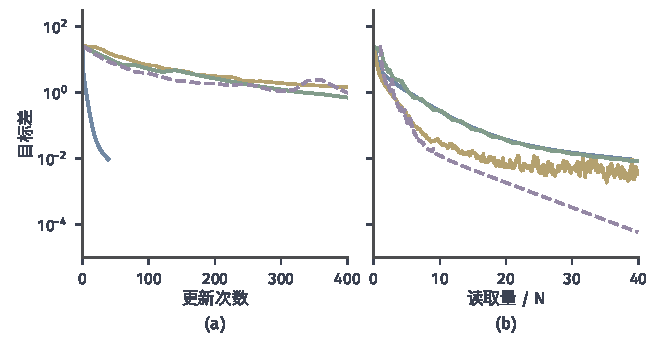
\includegraphics[width=112mm]{figures/05-optimization/05-stochastic-optimization/matplotlib/sgdb-cost-units/figure.pdf}
  \caption{同一个问题按不同单位的进展，有限和最小二乘加平方惩罚，$N=200$，$n=10$，$\gamma=0.1$。蓝线是步长$1/L$的全梯度下降，黄线是常步长随机梯度下降，绿线是SVRG，紫色虚线是SAGA。(a)横轴是参数更新次数。(b)横轴是样本读取量除以$N$，SVRG的快照和控制变量都计入读取量，SAGA的梯度表初始化也计入。}
  \label{fig:sgdb-cost-units}
\end{BookInlineFigure}

\paragraph{批量、微批量与历史更新的计时}
计时单位在调度中也要说明。步长调度按更新次数、样本读取量还是遍历次数推进，不同的实现可能相差一个批量大小的倍数。把一个批量拆成微批量累积梯度时，读取量不变，但更新次数减少；若统计量（比如批量内的归一化）按微批量更新，就要规定它的计时。

减少更新次数是否值得增加单步工作，取决于这次工作能否并行、读取是否昂贵、更新本身的成本。计算结论应写成“在某某单位下，某方法达到某精度需要多少”，不能只说某方法更快。

\subsection{样本替换的有限步响应}
\label{sec:sgdb-stability}

\paragraph{问题}
前面都固定了目标。现在换一个问题：两份数据只相差一个样本，让同一个算法在两份数据上运行，输出相差多少？这刻画的是算法这个从数据到输出的映射对单个样本有多敏感，称为\term{算法稳定性}（algorithmic stability）。

设目标$f$由$N$项平均而成，另一份数据的目标$\tilde f$只把第$k$项换成$\tilde f_k$，其余项相同。两次运行使用相同的初值、相同的步长序列，以及\emph{相同的}下标路径$i^{(0)},i^{(1)},\ldots$，得到$\bm{x}^{(t)}$和$\tilde{\bm x}^{(t)}$。这种做法称为耦合，它把抽样噪声的影响去掉，图~\ref{fig:sgdb-coupling}展示了它的结构：差异只在抽到第$k$项时产生。

\begin{BookInlineFigure}
  \centering
  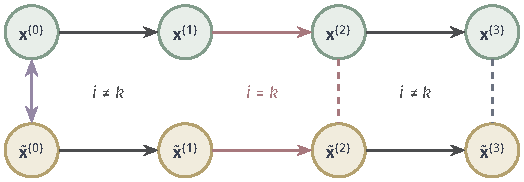
\includegraphics[width=88.74mm]{figures/05-optimization/05-stochastic-optimization/tikz/sgdb-coupling/figure.pdf}
  \caption{两次耦合运行。两条轨迹起点相同（紫色）。下标$i\neq k$时，两边用同一项更新，只传播已有差异；$i=k$时（红色箭头），两边用不同的项更新，新差异在此注入。}
  \label{fig:sgdb-coupling}
\end{BookInlineFigure}

\paragraph{用贯穿例计算}
取贯穿例，把第$3$项$f_3=\frac32(x-3)^2$换成$\tilde f_3=\frac32x^2$，也就是$b_3$从$3$变成$0$。起点都是$2$，$\alpha=0.1$，读取顺序为第$3,1,2$项，其中第一轮抽到被替换的项。两条轨迹依次是
\[
 \begin{aligned}
 x^{(1)}&=2.3, & \tilde x^{(1)}&=1.4, & \lvert x-\tilde x\rvert&=0.9,\\
 x^{(2)}&=1.77, & \tilde x^{(2)}&=0.96, & \lvert x-\tilde x\rvert&=0.81,\\
 x^{(3)}&=1.416, & \tilde x^{(3)}&=0.768, & \lvert x-\tilde x\rvert&=0.648.
 \end{aligned}
\]

第一轮两边的读数分别是$-3$和$6$，注入的差异是$0.1\cdot9=0.9$。后两轮用相同的项，$a_i=1,2$，差异分别乘以$1-\alpha a_i=0.9$和$0.8$，没有放大。下面的分析把这两种情形一般化。

\paragraph{传播：梯度步的非扩张}
先看未抽到被替换项的一步。两边用同一个函数走一步，距离不增加，这由下面的引理保证。这里为了证明简短，假定函数二阶连续可微。

\begin{lemma}[梯度步的非扩张与压缩]
\label{lem:sgdb-nonexpansive}
设$\phi$二阶连续可微，$\mu_0\bm{I}\preceq\nabla^2\phi\preceq L\bm{I}$，$\mu_0\geq0$。若$0<\alpha\leq2/(L+\mu_0)$，则对任意$\bm{x},\bm{y}$，
\begin{equation}
 \bigl\lVert\bigl(\bm{x}-\alpha\nabla\phi(\bm{x})\bigr)-\bigl(\bm{y}-\alpha\nabla\phi(\bm{y})\bigr)\bigr\rVert_2\leq(1-\alpha\mu_0)\lVert\bm{x}-\bm{y}\rVert_2 .
 \label{eq:sgdb-nonexpansive}
\end{equation}
\end{lemma}

\begin{proof}
由微积分基本定理，
\[
 \nabla\phi(\bm{x})-\nabla\phi(\bm{y})=\bm{A}(\bm{x}-\bm{y}),\qquad
 \bm{A}=\int_0^1\nabla^2\phi\bigl(\bm{y}+s(\bm{x}-\bm{y})\bigr)\,\mathrm{d}s .
\]

$\bm{A}$对称且$\mu_0\bm{I}\preceq\bm{A}\preceq L\bm{I}$。于是左端等于$\lVert(\bm{I}-\alpha\bm{A})(\bm{x}-\bm{y})\rVert_2$，矩阵$\bm{I}-\alpha\bm{A}$的特征值落在$[1-\alpha L,1-\alpha\mu_0]$内。条件$\alpha\leq2/(L+\mu_0)$保证$\alpha L-1\leq1-\alpha\mu_0$，所以这些特征值的绝对值不超过$1-\alpha\mu_0$，由此得到结论。
\end{proof}

\paragraph{注入与传播的合成}
差异只在抽到第$k$项时产生，每一步的概率是$1/N$。下面的定理把注入和传播合成一个界。

\begin{theorem}[样本替换下的期望参数距离]
\label{thm:sgdb-stability}
设每个$f_i$与$\tilde f_k$二阶连续可微，满足$\bm{0}\preceq\nabla^2\preceq L\bm{I}$。下标独立均匀抽取，确定的步长满足$0<\alpha^{(t)}\leq2/L$。设在两条轨迹访问的点上，被替换的两项梯度满足
\begin{equation}
 \lVert\nabla f_k(\bm{x}^{(t)})\rVert_2\leq G,\qquad \lVert\nabla\tilde f_k(\tilde{\bm x}^{(t)})\rVert_2\leq G .
 \label{eq:sgdb-stability-condition}
\end{equation}
则
\begin{equation}
 \mathbb{E}\lVert\bm{x}^{(T)}-\tilde{\bm x}^{(T)}\rVert_2\leq\frac{2G}{N}\sum_{t=0}^{T-1}\alpha^{(t)} .
 \label{eq:sgdb-stability}
\end{equation}
\end{theorem}

\begin{proof}
记两条轨迹的距离为
\[
 \delta^{(t)}=\lVert\bm{x}^{(t)}-\tilde{\bm x}^{(t)}\rVert_2,\qquad\delta^{(0)}=0.
\]

若$i^{(t)}\neq k$，两条轨迹用同一个$f_i$走一步，由引理~\ref{lem:sgdb-nonexpansive}（$\mu_0=0$），
\[
 \delta^{(t+1)}\leq\delta^{(t)} .
\]

若$i^{(t)}=k$，由三角不等式和式~\eqref{eq:sgdb-stability-condition}，
\[
 \delta^{(t+1)}\leq\delta^{(t)}+\alpha^{(t)}\bigl(\lVert\nabla f_k(\bm{x}^{(t)})\rVert_2+\lVert\nabla\tilde f_k(\tilde{\bm x}^{(t)})\rVert_2\bigr)\leq\delta^{(t)}+2\alpha^{(t)}G .
\]

下标与历史独立，后一种情形的条件概率是$1/N$，所以
\[
 \mathbb{E}\bigl[\delta^{(t+1)}\mid\mathcal{F}^{(t)}\bigr]\leq\delta^{(t)}+\frac{2\alpha^{(t)}G}{N}.
\]

取全期望，对$t=0,\ldots,T-1$累加，得到式~\eqref{eq:sgdb-stability}。
\end{proof}

这个界的结构是：每步以概率$1/N$注入不超过$2\alpha^{(t)}G$的差异，注入后的差异不再放大。若每项还$\mu_0$强凸，$\mu_0>0$，$\alpha\leq2/(L+\mu_0)$，引理给出的压缩因子就进入递推，常步长下
\[
 \mathbb{E}\delta^{(t+1)}\leq(1-\alpha\mu_0)\mathbb{E}\delta^{(t)}+\frac{2\alpha G}{N},
\]
它的极限不超过$2G/(N\mu_0)$，界不再随$T$无限增长。图~\ref{fig:sgdb-stability-run}(b)显示了实际平均距离与两条界：实际距离上升到约$0.04$后回落并稳定，远低于两条上界。上界偏保守的一个原因是$G$取了路径上的最大值，而实际注入的差异通常小于$2\alpha G$。

\begin{BookInlineFigure}
  \centering
  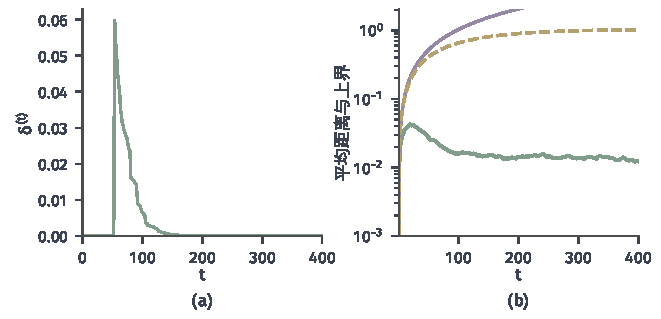
\includegraphics[width=112mm]{figures/05-optimization/05-stochastic-optimization/matplotlib/sgdb-stability-run/figure.pdf}
  \caption{样本替换的有限步响应，平方损失加平方惩罚的$N=100$项平均，$\gamma=0.2$，常步长$1/L_{\max}$，第$1$项被替换。(a)一条耦合路径上的距离$\delta^{(t)}$：抽到被替换项时跳起，之后逐渐压缩。(b)$1500$对路径的平均距离（绿），式~\eqref{eq:sgdb-stability}的非扩张界（紫）与利用强凸的压缩界（黄色虚线）。}
  \label{fig:sgdb-stability-run}
\end{BookInlineFigure}

\paragraph{结论的适用范围}
逐项的条件要逐一核对。这里要求的是每一项凸且光滑，只有平均目标凸是不够的，否则未抽到被替换项的那一步也可能拉开距离。凸性和步长决定传播：目标不凸时，梯度步可以把差异放大到$1+\alpha L$倍；步长超过$2/L$时，即使凸函数的梯度步也可能扩张。梯度界$G$只需要在实际访问的点上成立；对最小二乘这样的目标，它依赖轨迹所停留的区域。去掉二阶可微条件时，凸$L$光滑函数的梯度步仍然非扩张，证明需要梯度的余强制性，篇幅较长，读者可查阅\scite{hardt2016sgd}。

式~\eqref{eq:sgdb-stability}说的是参数的距离。要把它转成损失的变化，还需要损失对参数的定量控制：若损失关于参数$K$-Lipschitz，则损失之差不超过$K\lVert\bm{x}^{(T)}-\tilde{\bm x}^{(T)}\rVert_2$。这是另一个独立的条件。从算法的输出差异到统计泛化结论，还要有样本分布和数据生成假设，这部分不在有限步优化的范围内。

\section{本章小结}
\label{sec:sgd-summary}

本章回答了一个问题：不读全部目标项时，怎样构造更新并判断它的结果。抽样决定读取哪些项，读数的条件无偏是一切分析的起点，但单步读数可能指向上升方向，要靠期望递推和步长控制来管理噪声。

方差控制决定怎样利用额外读取和记忆。小批量、非均匀抽样和控制变量都能减小读数的方差，代价是快照、梯度表或抽样分布的维护。方差减小并不等同于总计算减少，要按相同的目标和精度比较。

动量、自适应尺度和方向处理分别改变实际更新的不同环节。动量把历史读数合成方向，平滑噪声的同时带来滞后，它对当前梯度不是无偏的，常步长下的噪声残余由有效步长决定。Nesterov方法的读数对应前瞻点，确定性的加速不能直接继承，噪声在势函数中留下不随步数消失的项。Lion与Muon对动量做非线性变换，分别舍弃坐标和奇异方向的幅度，实际位移、原目标残差和矩阵运算成本要分开核对。

自适应方法用历史幅度决定尺度。AdaGrad累计平方而难以遗忘，RMSProp用指数平均，Adam再加上方向平均和零初始化修正，AMSGrad让分母单调，AdamW把收缩与统计分开，Adafactor和Shampoo处理矩阵参数的存储和方向关系。这些尺度通常依赖当前读数，每种保证都必须连同它的假设一起引用，单调性之类的代数性质不是收敛结论。

裁剪、近似和替代让实际方向偏离梯度。把读数分解为真梯度、条件偏差和噪声，就能看到噪声项随步长缩小，偏差项不随步长缩小，而上界中的残余不一定是实际的下限。替代方向不是原目标的导数，评价和停止都要回到实际的前向目标。

所有保证都对应一个具体的目标、一个返回点和一个计算单位。同一个问题按更新次数和按读取量计时，方法的排序可以不同。有限步优化误差、路径的长期收敛和样本造成的统计误差是三个不同的问题，本章处理的是第一个，只说明了另外两个与它的分工。样本替换的分析则把算法看作从数据到输出的映射，为后续讨论统计误差提供了一种输入。

随机梯度方法需要目标的梯度读数。若只能读到函数值，就要先由函数值构造方向，下一章研究这个问题。

